% Options for packages loaded elsewhere
\PassOptionsToPackage{unicode}{hyperref}
\PassOptionsToPackage{hyphens}{url}
%
\documentclass[
]{book}
\usepackage{amsmath,amssymb}
\usepackage{iftex}
\ifPDFTeX
  \usepackage[T1]{fontenc}
  \usepackage[utf8]{inputenc}
  \usepackage{textcomp} % provide euro and other symbols
\else % if luatex or xetex
  \usepackage{unicode-math} % this also loads fontspec
  \defaultfontfeatures{Scale=MatchLowercase}
  \defaultfontfeatures[\rmfamily]{Ligatures=TeX,Scale=1}
\fi
\usepackage{lmodern}
\ifPDFTeX\else
  % xetex/luatex font selection
\fi
% Use upquote if available, for straight quotes in verbatim environments
\IfFileExists{upquote.sty}{\usepackage{upquote}}{}
\IfFileExists{microtype.sty}{% use microtype if available
  \usepackage[]{microtype}
  \UseMicrotypeSet[protrusion]{basicmath} % disable protrusion for tt fonts
}{}
\makeatletter
\@ifundefined{KOMAClassName}{% if non-KOMA class
  \IfFileExists{parskip.sty}{%
    \usepackage{parskip}
  }{% else
    \setlength{\parindent}{0pt}
    \setlength{\parskip}{6pt plus 2pt minus 1pt}}
}{% if KOMA class
  \KOMAoptions{parskip=half}}
\makeatother
\usepackage{xcolor}
\usepackage{color}
\usepackage{fancyvrb}
\newcommand{\VerbBar}{|}
\newcommand{\VERB}{\Verb[commandchars=\\\{\}]}
\DefineVerbatimEnvironment{Highlighting}{Verbatim}{commandchars=\\\{\}}
% Add ',fontsize=\small' for more characters per line
\usepackage{framed}
\definecolor{shadecolor}{RGB}{248,248,248}
\newenvironment{Shaded}{\begin{snugshade}}{\end{snugshade}}
\newcommand{\AlertTok}[1]{\textcolor[rgb]{0.94,0.16,0.16}{#1}}
\newcommand{\AnnotationTok}[1]{\textcolor[rgb]{0.56,0.35,0.01}{\textbf{\textit{#1}}}}
\newcommand{\AttributeTok}[1]{\textcolor[rgb]{0.13,0.29,0.53}{#1}}
\newcommand{\BaseNTok}[1]{\textcolor[rgb]{0.00,0.00,0.81}{#1}}
\newcommand{\BuiltInTok}[1]{#1}
\newcommand{\CharTok}[1]{\textcolor[rgb]{0.31,0.60,0.02}{#1}}
\newcommand{\CommentTok}[1]{\textcolor[rgb]{0.56,0.35,0.01}{\textit{#1}}}
\newcommand{\CommentVarTok}[1]{\textcolor[rgb]{0.56,0.35,0.01}{\textbf{\textit{#1}}}}
\newcommand{\ConstantTok}[1]{\textcolor[rgb]{0.56,0.35,0.01}{#1}}
\newcommand{\ControlFlowTok}[1]{\textcolor[rgb]{0.13,0.29,0.53}{\textbf{#1}}}
\newcommand{\DataTypeTok}[1]{\textcolor[rgb]{0.13,0.29,0.53}{#1}}
\newcommand{\DecValTok}[1]{\textcolor[rgb]{0.00,0.00,0.81}{#1}}
\newcommand{\DocumentationTok}[1]{\textcolor[rgb]{0.56,0.35,0.01}{\textbf{\textit{#1}}}}
\newcommand{\ErrorTok}[1]{\textcolor[rgb]{0.64,0.00,0.00}{\textbf{#1}}}
\newcommand{\ExtensionTok}[1]{#1}
\newcommand{\FloatTok}[1]{\textcolor[rgb]{0.00,0.00,0.81}{#1}}
\newcommand{\FunctionTok}[1]{\textcolor[rgb]{0.13,0.29,0.53}{\textbf{#1}}}
\newcommand{\ImportTok}[1]{#1}
\newcommand{\InformationTok}[1]{\textcolor[rgb]{0.56,0.35,0.01}{\textbf{\textit{#1}}}}
\newcommand{\KeywordTok}[1]{\textcolor[rgb]{0.13,0.29,0.53}{\textbf{#1}}}
\newcommand{\NormalTok}[1]{#1}
\newcommand{\OperatorTok}[1]{\textcolor[rgb]{0.81,0.36,0.00}{\textbf{#1}}}
\newcommand{\OtherTok}[1]{\textcolor[rgb]{0.56,0.35,0.01}{#1}}
\newcommand{\PreprocessorTok}[1]{\textcolor[rgb]{0.56,0.35,0.01}{\textit{#1}}}
\newcommand{\RegionMarkerTok}[1]{#1}
\newcommand{\SpecialCharTok}[1]{\textcolor[rgb]{0.81,0.36,0.00}{\textbf{#1}}}
\newcommand{\SpecialStringTok}[1]{\textcolor[rgb]{0.31,0.60,0.02}{#1}}
\newcommand{\StringTok}[1]{\textcolor[rgb]{0.31,0.60,0.02}{#1}}
\newcommand{\VariableTok}[1]{\textcolor[rgb]{0.00,0.00,0.00}{#1}}
\newcommand{\VerbatimStringTok}[1]{\textcolor[rgb]{0.31,0.60,0.02}{#1}}
\newcommand{\WarningTok}[1]{\textcolor[rgb]{0.56,0.35,0.01}{\textbf{\textit{#1}}}}
\usepackage{longtable,booktabs,array}
\usepackage{calc} % for calculating minipage widths
% Correct order of tables after \paragraph or \subparagraph
\usepackage{etoolbox}
\makeatletter
\patchcmd\longtable{\par}{\if@noskipsec\mbox{}\fi\par}{}{}
\makeatother
% Allow footnotes in longtable head/foot
\IfFileExists{footnotehyper.sty}{\usepackage{footnotehyper}}{\usepackage{footnote}}
\makesavenoteenv{longtable}
\usepackage{graphicx}
\makeatletter
\def\maxwidth{\ifdim\Gin@nat@width>\linewidth\linewidth\else\Gin@nat@width\fi}
\def\maxheight{\ifdim\Gin@nat@height>\textheight\textheight\else\Gin@nat@height\fi}
\makeatother
% Scale images if necessary, so that they will not overflow the page
% margins by default, and it is still possible to overwrite the defaults
% using explicit options in \includegraphics[width, height, ...]{}
\setkeys{Gin}{width=\maxwidth,height=\maxheight,keepaspectratio}
% Set default figure placement to htbp
\makeatletter
\def\fps@figure{htbp}
\makeatother
\setlength{\emergencystretch}{3em} % prevent overfull lines
\providecommand{\tightlist}{%
  \setlength{\itemsep}{0pt}\setlength{\parskip}{0pt}}
\setcounter{secnumdepth}{5}
\usepackage{booktabs}
\ifLuaTeX
  \usepackage{selnolig}  % disable illegal ligatures
\fi
\usepackage[]{natbib}
\bibliographystyle{apalike}
\IfFileExists{bookmark.sty}{\usepackage{bookmark}}{\usepackage{hyperref}}
\IfFileExists{xurl.sty}{\usepackage{xurl}}{} % add URL line breaks if available
\urlstyle{same}
\hypersetup{
  pdftitle={Bayesian Inference and Computation},
  pdfauthor={Dr Rowland Seymour},
  hidelinks,
  pdfcreator={LaTeX via pandoc}}

\title{Bayesian Inference and Computation}
\author{Dr Rowland Seymour}
\date{Semester 2, 2024}

\usepackage{amsthm}
\newtheorem{theorem}{Theorem}[chapter]
\newtheorem{lemma}{Lemma}[chapter]
\newtheorem{corollary}{Corollary}[chapter]
\newtheorem{proposition}{Proposition}[chapter]
\newtheorem{conjecture}{Conjecture}[chapter]
\theoremstyle{definition}
\newtheorem{definition}{Definition}[chapter]
\theoremstyle{definition}
\newtheorem{example}{Example}[chapter]
\theoremstyle{definition}
\newtheorem{exercise}{Exercise}[chapter]
\theoremstyle{definition}
\newtheorem{hypothesis}{Hypothesis}[chapter]
\theoremstyle{remark}
\newtheorem*{remark}{Remark}
\newtheorem*{solution}{Solution}
\begin{document}
\maketitle

{
\setcounter{tocdepth}{1}
\tableofcontents
}
\hypertarget{practicalities}{%
\chapter*{Practicalities}\label{practicalities}}
\addcontentsline{toc}{chapter}{Practicalities}

\hypertarget{module-aims}{%
\section{Module Aims}\label{module-aims}}

Bayesian inference is a set of methods where the probability of an event
occurring can be updated as more information becomes available. It is
fundamentally different from frequentist methods, which are based on
long running relative frequencies. This module gives an introduction to
the Bayesian approach to statistical analysis and the theory that
underpins it.

Students will be able to explain the distinctive features of Bayesian
methodology, understand and appreciate the role of prior distributions
and compute posterior distributions. It will cover the derivation of
posterior distributions, the construction of prior distributions, and
inference for missing data. Extensions are considered to models with
more than a single parameter and how these can be used to analyse data.
Computational methods have greatly advanced the use of Bayesian methods
and this module covers, and allows students to apply, procedures for the
sampling and analysis of intractable Bayesian problems.

By the end of the course, students should be able to:

\begin{enumerate}
\def\labelenumi{\arabic{enumi}.}
\tightlist
\item
  Demonstrate a full and rigorous understanding of all definitions
  associated with Bayesian inference and understand the differences
  between the Bayesian and frequentist approaches to inference
\item
  Demonstrate a sound understanding of the fundamental concepts of
  Bayesian inference and computational sampling methods
\item
  Understand how to make inferences assuming various population
  distributions while taking into account expert opinion and the
  implications of weak prior knowledge and large samples
\item
  Demonstrate an understanding of the principles of Markov Chain Monte
  Carlo and be able to programme an MCMC algorithm
\item
  Engage in Bayesian data analysis in diverse situations drawn from
  physics, biological, engineering and other mathematical contexts.
\end{enumerate}

\hypertarget{module-structure}{%
\section{Module Structure}\label{module-structure}}

The module is split between theory and computation. Each week will have three lectures, one computer lab and one guided study. In the labs, you will need to bring your own laptop. The timetable for this module is

\begin{longtable}[]{@{}
  >{\raggedright\arraybackslash}p{(\columnwidth - 8\tabcolsep) * \real{0.0833}}
  >{\raggedright\arraybackslash}p{(\columnwidth - 8\tabcolsep) * \real{0.2500}}
  >{\raggedright\arraybackslash}p{(\columnwidth - 8\tabcolsep) * \real{0.2222}}
  >{\raggedright\arraybackslash}p{(\columnwidth - 8\tabcolsep) * \real{0.2361}}
  >{\raggedright\arraybackslash}p{(\columnwidth - 8\tabcolsep) * \real{0.2083}}@{}}
\toprule\noalign{}
\begin{minipage}[b]{\linewidth}\raggedright
Week
\end{minipage} & \begin{minipage}[b]{\linewidth}\raggedright
Monday (1200)
\end{minipage} & \begin{minipage}[b]{\linewidth}\raggedright
Tuesday (1000)
\end{minipage} & \begin{minipage}[b]{\linewidth}\raggedright
Thursday (1100)
\end{minipage} & \begin{minipage}[b]{\linewidth}\raggedright
Friday (1200)
\end{minipage} \\
\midrule\noalign{}
\endhead
\bottomrule\noalign{}
\endlastfoot
2 & Physics West 115 & Nuffield G18 & Nuffield G13 & Nuffield G19 \\
3 & Physics West 115 & Nuffield G18 & Arts LR5 & Nuffield G19 \\
4 & Physics West 115 & Nuffield G18 & Nuffield G13 & Nuffield G13 \\
5 & Physics West 115 & Nuffield G18 & Arts LR5 & Nuffield G19 \\
6 & Physics West 115 & Nuffield G18 & Nuffield G13 & Nuffield G13 \\
7 & Physics West 115 & Nuffield G18 & Nuffield G13 & Nuffield G13 \\
8 & Physics West 115 & Nuffield G18 & Arts LR5 & Nuffield G19 \\
9 & Physics West 115 & Nuffield G18 & Nuffield G13 & Nuffield G19 \\
10 & Physics West 115 & Nuffield G18 & Nuffield G13 & Nuffield G13 \\
\end{longtable}

\hypertarget{assessment}{%
\section{Assessment}\label{assessment}}

Assessment for this module is 50\% via an exam and 50\% via coursework
assignments during the semester. The exam will last 1h 30m and take
place during the summer exam period. There will be three coursework
assignment -- assignment 1 will be worth 10\% of the final mark, with
assignments 2 and 3 counting for 20\% each. More details about the
assignments will be made available during the semester.

\hypertarget{getting-help}{%
\section{Getting Help}\label{getting-help}}

There are lots of ways of getting help throughout the module. You can
visit my office hour (Watson 317) on Thursdays at 0900-1030 or email me at
\href{mailto:r.g.seymour@bham.ac.uk}{\nolinkurl{r.g.seymour@bham.ac.uk}}.

\hypertarget{recommended-books-and-videos}{%
\section{Recommended Books and Videos}\label{recommended-books-and-videos}}

No books are required for this course and the whole material is
contained in these notes. However, you may find it useful to use other
resources in your studies. I recommend the following:

\begin{enumerate}
\def\labelenumi{\arabic{enumi}.}
\item
  \href{https://link.springer.com/book/10.1007/978-0-387-92407-6}{A First Course in Bayesian Statistical Methods - Peter D.
  Hoff}.
  This is a short book that covers the basics of Bayesian inference
  and computation. To the point and well written, it's a useful place
  to look topics up.
\item
  \href{http://www.stat.columbia.edu/~gelman/book/}{Bayesian Data Analysis - Andrew Gelman, John Carlin, Hal Stern,
  David Dunson, Aki Vehtari, and Donald
  Rubin}. This is a
  thorough book explaining everything you'd need to know to carry out
  Bayesian data analysis. It's a fairly long and in-depth book, but
  the authors are authoritative and give good advice throughout.
  Example code on the website is in R, Python and Stan.
\item
  \href{https://xcelab.net/rm/statistical-rethinking/}{Statistical Rethinking - Richard
  McElrath}. This book
  provides a friendly intuitive understanding of Bayesian inference
  and computation. Aimed at social and natural scientists, it has less
  theory that the other two books but is perhaps more approachable. A
  set of video lectures for this book can be found on
  \href{https://www.youtube.com/playlist?list=PLDcUM9US4XdMROZ57-OIRtIK0aOynbgZN}{YouTube}.
\end{enumerate}

\hypertarget{common-distributions}{%
\section{Common Distributions}\label{common-distributions}}

For many Bayesian inference problems, it is useful to be able to
identify probability density functions (for continuous random variables)
and probability mass functions (for discrete random variables) up to
proportionality. Some common density/mass functions are given below.

\textbf{Normal distribution} \[
\pi(x \mid \mu, \sigma^2) = \frac{1}{\sqrt{2\pi\sigma^2}}\exp\left\{-\frac{1}{2\sigma^2}(x-\mu)^2\right\} \qquad x \in\mathbb{R},
\] where \(\mu \in \mathbb{R}\) and \(\sigma > 0\).

\textbf{Beta distribution} \[
\pi(x\mid \alpha, \beta) = \frac{1}{B(\alpha, \beta)}x^{\alpha-1}(1-x)^{\beta - 1} \qquad  x \in [0, 1],
\] where \(\alpha, \beta > 0\) and \(B(\alpha, \beta)\) is the \href{https://en.wikipedia.org/wiki/Beta_function}{beta
function}.

\textbf{Gamma distribution} \[
\pi(x\mid \alpha, \beta) = \frac{\beta^\alpha}{\Gamma(\alpha)}x^{\alpha - 1}e^{-\beta x} \qquad  x > 0,
\] where \(\alpha, \beta > 0\) and \(\Gamma(\alpha)\) is the \href{https://en.wikipedia.org/wiki/Gamma_function}{gamma
function}.

\textbf{Exponential distribution} \[
f(x \mid \lambda) = \lambda e^{-\lambda x} \qquad x > 0,
\] where \(\lambda > 0\).

\textbf{Poisson distribution} \[
\pi(x = k \mid \lambda) = \frac{\lambda^k e^{-\lambda}}{k!} \qquad k \in \{1, 2, \ldots\},
\] where \(\lambda > 0\).

\textbf{Binomial distribution} \[
\pi(x = k \mid N, p) = \begin{pmatrix} N \\ k\end{pmatrix} p^k (1-p)^{N-k} \qquad k \in \{1, \ldots, N\}
\] where \(p \in [0, 1]\).

\hypertarget{fundamentals}{%
\chapter{Fundamentals of Bayesian Inference}\label{fundamentals}}

Bayesian inference is built on a different way of thinking about parameters of probability distributions than methods you have learnt so far. In the past 30 years or so, Bayesian inference has become much more popular. This is partly due to increased computational power becoming available. In this first chapter, we are going to set out to answer:

\begin{enumerate}
\def\labelenumi{\arabic{enumi}.}
\item
  What are the fundamental principles of Bayesian inference?
\item
  What makes Bayesian inference different from other methods?
\end{enumerate}

\hypertarget{statistical-inference}{%
\section{Statistical Inference}\label{statistical-inference}}

The purpose of statistical inference is to ``draw conclusions, from numerical data, about quantities that are not observed'' (Bayesian Data Analysis, chapter 1). Generally speaking, there are two kinds of inference:

\begin{enumerate}
\def\labelenumi{\arabic{enumi}.}
\tightlist
\item
  Inference for quantities that are unobserved or haven't happened yet. Examples of this might be the size of a payout an insurance company has to make, or a patients outcome in a clinical trial had they been received a certain treatment.
\item
  Inference for quantities that are not possible to observe. This is usual because they are part of modelling process, like parameters in a linear model.
\end{enumerate}

In this module, we are going to look at a different way of carrying out statistical inference, one that doesn't depend on long run events. Instead, we're going to introduce the definition of probability that allows us to interpret the subjective chance that an event occurs.

\hypertarget{frequentist-theory}{%
\section{Frequentist Theory}\label{frequentist-theory}}

Frequentist probability is built upon the theory on long run events. Probabilities must be interpretable as frequencies over multiple repetitions of the experiment that is being analysed, and are calculated from the sampling distributions of measured quantities.

\begin{definition}
The long run relative frequency of an event is the \textbf{probability} of that event.
\end{definition}

\begin{example}
If a frequentist wanted to assign a probability to rolling a 6 on a particular dice, then they would roll the dice a large number of times and compute the relative frequency.
\end{example}

\begin{definition}
The \textbf{sampling distribution} of a statistic is the distribution based on a long run of samples of a fixed size from the population.
\end{definition}

The sampling distribution is an important concept in frequentist theory as it describes the randomness in the process. From a frequentist standpoint, we have a model containing some parameter \(\theta\) and some data \(\boldsymbol{y}\). All the evidence in the data \(\boldsymbol{y}\) about \(\theta\) is contained in the likelihood function \(\pi(\boldsymbol{y} \mid \theta)\). The parameter \(\theta\) is fixed and the likelihood function describes the probability of observing the data \(\boldsymbol{y}\) given the parameter \(\theta\).

The most common way to estimate the value of \(\theta\) is using maximum likelihood estimation. Although other methods do exist (e.g.~method of moments, or generalised maximum likelihood estimation).

\begin{definition}
The maximum likelihood estimate of \(\theta\), \(\hat{\theta}\), is the value such that \(\hat{\theta} = \max_{\theta} \pi(\boldsymbol{y}\mid \theta)\).
\end{definition}

Uncertainty around the maximum likelihood estimate is based on the theory of long running events that underpin frequentist theory.

\begin{definition}
Let \(Y\) be a random sample from a probability distribution \(\theta\). A \(100(1-\alpha)%
\) \textbf{confidence interval} for \(\theta\) is an interval \((u(Y), v(Y))\) such that
\[
\mathbb{P}(u(Y) < \theta < v(Y)) = 1-\alpha
\]
\end{definition}

This means that if you had an infinite number of samples for \(Y\) and the corresponding infinite number of confidence intervals, then \(100(1-\alpha)\)\% of them would contain the true value of \(\theta\). It does \emph{not} mean that there is a \(100(1-\alpha)\) probability a particular interval contains the true value of \(\theta\).

Given that we want to understand the properties of \(\theta\) given the data we have observed \(\boldsymbol{y}\), then you might think it makes sense to investigate the distribution \(\pi(\theta \mid \boldsymbol{y})\). This distribution says what are the likely values of \(\theta\) given the information we have observed from the data \(\boldsymbol{y}\). We will talk about Bayes' theorem in more detail later on in this chapter, but, for now, we will use it to write down this distribution
\[
\pi(\theta \mid \boldsymbol{y}) = \frac{\pi(\boldsymbol{y} \mid \theta)\pi(\theta)}{\pi(\boldsymbol{y})}. 
\]
This is where frequentist theory cannot help us, particularly the term \(\pi(\theta)\). Randomness can only come from the data, so how can we assign a probability distribution to a constant \(\theta\)? The term \(\pi(\theta)\) is meaningless under this philosophy. Instead, we turn to a different philosophy where we can assign a probability distribution to \(\theta\).

\hypertarget{bayesian-probability}{%
\section{Bayesian Probability}\label{bayesian-probability}}

The Bayesian paradigm is built around a different definition of probability. This allows us to generate probability distirbutuions for parameters values.

\begin{definition}
The subjective belief of an event is the \textbf{probability} of that event.
\end{definition}

This definition means we can assign probabilities to events that frequentists do not recognise as valid.

\begin{example}
Consider the following:

\begin{enumerate}
\def\labelenumi{\arabic{enumi}.}
\item
  The probability that I vote for the labour party at the next election
\item
  A photo taken from the James Watt telescope contains a new planet.
\item
  The real identify of Banksy is Robin Gunningham.
\end{enumerate}

These are not events that can be repeated in the long run.
\end{example}

\hypertarget{conditional-probability-and-exchangability}{%
\section{Conditional Probability and Exchangability}\label{conditional-probability-and-exchangability}}

Before we derive Bayes' theorem, we recap some important definitions in probability.

\begin{definition}
Given two events \(A\) and \(B\), the \textbf{conditional probability} that event \(A\) occurs given the event \(B\) has already occurred is
\[
\pi(A \mid B) = \frac{\pi(A \cap B)}{\pi(B)}, 
\]
when \(\pi(B) > 0\).
\end{definition}

\begin{definition}
Two events \(A\) and \(B\) are \textbf{independent} given event \(C\) if and only if
\[ \pi(A \cap B \mid C) = \pi(A \mid C)\pi(B \mid C).\]
\end{definition}

\begin{definition}
Let \(\pi(y_1, \ldots, y_N)\) be the joint density of \(Y_1, \ldots, Y_N\). If \(\pi(y_1, \ldots, y_N) = \pi(y_{\pi_1}, \ldots, y_{\pi_N})\) for a permutations \(\pi\) of \(\{1, \ldots, N\}\), then \(Y_1, \ldots, Y_N\) are \textbf{exchangeable}.
\end{definition}

Exchangability means that the labels of the random variables don't contain any information about the outcomes. This is an important idea in many areas of probability and statistics, and we often model exchangeable events as iid.

\begin{example}
If \(Y_i \sim Bin(n, p)\) are independent and identically distributed for \(i = 1, 2, 3\), then \(\pi(Y_1, Y_2, Y_3) = \pi(Y_3, Y_1, Y_2)\).
\end{example}

\begin{example}
Let \((X, Y)\) follow a bivariate normal distribution with mean \textbf{0}, variances \(\sigma_x = \sigma_y = 1\) and a correlation parameter \(\rho \in [-1, 1]\). \((X, Y)\) are exchangable, but only independent if \(\rho = 0\).
\end{example}

\begin{proposition}
If \(\theta \sim \pi(\theta)\) and \((Y_1, \ldots, Y_N)\) from a sample space \(\mathcal{Y}\) are conditionally iid given some parameter \(\theta\), then marginally \(Y_1, \ldots, Y_N\) are exchangable.
\end{proposition}

\begin{proof}
Suppose \((Y_1, \ldots, Y_N)\) are conditionally iid given some parameter \(\theta\). Then for any permutation \(\sigma\) of \(\{1, \ldots, N\}\) and observations \(\{y_1, \ldots, y_N\}\)
\begin{equation}
\begin{split}
\pi(y_1, \ldots, y_N) &= \int \pi(y_1, \ldots, y_N \mid \theta) \pi(\theta)\, d\theta \qquad \textrm{(definition of marginal distribution)}\\
 & = \int \left\{\prod_{i=1}^N\pi(y_i \mid \theta)\right\} \pi(\theta)\, d\theta \qquad \textrm{(definition of conditionally iid)}\\
& = \int \left\{\prod_{i=1}^N\pi(y_{\sigma_i} \mid \theta)\right\} \pi(\theta)\, d\theta \qquad \textrm{(product is commutative)} \\
 & = \pi(y_{\pi_1}, \ldots, y_{\sigma_N}) \qquad \textrm{(definition of marginal distribution)}
\end{split}
\end{equation}
\end{proof}

This tells us that if we have some conditionally iid random variables and a subjective prior belief about some parameter \(\theta\), then we have exchangeability. This is nice to have, but the implication in the other direction is much more interesting and powerful.

\begin{theorem}[de Finetti]
If a sequence of random variables \((Y_1, \ldots, Y_N)\) from a sample space \(\mathcal{Y}\) is exchangeable, then its joint distribution can be written as
\[
\pi(y_1, \ldots, y_N) = \int \left\{\prod_{i=1}^N\pi(y_i \mid \theta)\right\} \pi(\theta)\, d\theta
\]
for some parameter \(\theta\), some distribution on \(\theta\), and some sampling model \(\pi(y_i \mid \theta)\).
\end{theorem}

This is a kind of existence theorem for Bayesian inference. It says that if we have exchangeable random varibales, then a parameter \(\theta\) must exist and a subjective probability distribution \(\pi(\theta)\) must also exist. The argument against Bayesian inference is that it doesn't guarantee a \emph{good} subjective probability distribution \(\pi(\theta)\) exists.

\hypertarget{bayes-theorem}{%
\section{Bayes' Theorem}\label{bayes-theorem}}

Now we have an understanding of conditional probability and exchangeability, we can put these two together to understand Bayes' Theorem. Bayes' theorem is concerned with the distribution of the parameter \(\theta\) given some observed data \(y\). It tries to answer the question: what does the data tell us about the model parameters?

\begin{theorem}[Bayes]
The distribution of the model parameter \(\theta\) given the data \(y\) is
\[
\pi(\theta \mid y) = \frac{\pi(y \mid \theta)\pi(\theta)}{\pi(y)}
\]
\end{theorem}

\begin{proof}
\begin{align}
\pi(\theta \mid y) &= \frac{\pi(\theta, y)}{\pi(y)}\\
\implies \pi(\theta, y) &= \pi(\theta \mid y)\pi(y)
\end{align}
Analogously, using \(\pi(y \mid \theta)\) we can derive
\[
\pi(\theta, y) = \pi(y \mid \theta)\pi(\theta)
\]
Putting these two terms equal to each other and dividing by \(\pi(y)\) gives
\[
\pi(\theta \mid y) = \frac{\pi(y \mid \theta)\pi(\theta)}{\pi(y)}
\]
\end{proof}

There are four terms in Bayes' theorem:

\begin{enumerate}
\def\labelenumi{\arabic{enumi}.}
\tightlist
\item
  The \textbf{posterior distribution} \(\pi(\theta \mid y)\). This tells us our belief about the model parameter \(\theta\) given the data we have observed \(y\).
\item
  The \textbf{likelihood function} \(\pi(y \mid \theta)\). The likelihood function is common to both frequentist and Bayesian methods. By the likelihood principle, the likelihood function contains all the information the data can tell us about the model parameter \(\theta\).
\item
  The \textbf{prior distribution} \(\pi(\theta)\). This is the distribution that describes our prior beliefs about the value of \(\theta\). The form of \(\theta\) should be decided before we see the data. It may be a vague distribution (e.g.~\(\theta \sim N(0, 10^2)\)) or a specific distribution based on prior information from experts (e.g.~\(\theta \sim N(5.5, 1.3^2)\)).\\
\item
  The \textbf{evidence of the data} \(\pi(y)\). This is sometimes called the average probability of the data or the marginal likelihood. In practice, we do not need to derive this term as it can be back computed to ensure the posterior distribution sums/integrates to one.
\end{enumerate}

A consequence of point four is that posterior distributions are usually derived proportionally, and (up to proportionality) Bayes' theorem
\[
\pi(\theta \mid y) \propto \pi(y\mid\theta)\pi(\theta).
\]

\begin{quote}
\textbf{Some history of Thomas Bayes}. Thomas Bayes was an English theologean born in 1702. His ``Essay towards solving a problem in the doctrine of chances'' was published posthumously. It introduces theroems on conditional probability and the idea of prior probability. He discusses an experiment where the data can be modelled using the Binomial distribution and he guesses (places a prior distribution) on the probability of success.
\end{quote}

\begin{quote}
Richard Price sent Bayes' work to the Royal Society two years after Bayes had died. In his commentary on Bayes' work, he suggested that the Bayesian way of thinking proves the existance of God, stating: The purpose I mean is, to show what reason we have for believing that there are in the constitution of things fixt laws according to which things happen, and that, therefore, the frame of the world must be the effect of the wisdom and power of an intelligent cause; and thus to confirm the argument taken from final causes for the existence of the Deity.
\end{quote}

\begin{quote}
It's not clear how Bayesian Thomas Bayes actually was, as his work was mainly about specific forms of probability theory and not his intepretation of it. The Bayesian way of thinking was really popularised by Laplace, who wrote about deductive probability in the early 19th century.
\end{quote}

\begin{example}

We finish this chapter with a very simple example. The advantage of the example being so simple is that we can obtain plots in R that show what's going on.

Suppose we have a model \(y \sim N(\theta, 1)\) and we want to estimate \(\theta\). To do this we need to derive the posterior distribution. By Bayes' theorem,
\[
\pi(\theta \mid y) \propto \pi(y \mid \theta) \pi(\theta).
\]
We know the form of \(\pi(y \mid \theta) = \frac{1}{\sqrt{2\pi}}e^{-\frac{1}{2}(y - \theta)^2}\), but how should we describe our prior beliefs about \(\theta\)? Here are three options:

\begin{enumerate}
\def\labelenumi{\arabic{enumi}.}
\item
  We can be very vague about \(\theta\) -- we genuinely don't know about its value. We assign a uniform prior distribution to \(\theta\) that takes values between -1,000 and +1,000, i.e.~\(\theta \sim u[-1000, 1000]\). Up to proportionality \(\pi(\theta) \propto 1\) for \(\theta \in [-1000, 1000]\).
\item
  After thinking hard about the problem, or talking to an expert, we decide that the only thing we know about \(\theta\) is that it can't be negative. We adjust our prior distribution from 1. to be \(\theta \sim u[0, 1000]\). Up to proportionality \(\pi(\theta) \propto 1\) for \(\theta \in [0, 1000]\).
\item
  We decide to talk to a series of experts about \(\theta\) asking for their views on likely values of \(\theta\). Averaging the experts opinions gives \(\theta \sim N(3, 0.7^2)\). This is a method known as prior elicitation.
\end{enumerate}

We now go and observe some data. After a lot of time and effort, we collect one data point: \(y = 0\).

Now we have all the ingredients to construct the posterior distribution. We multiply the likelihood function evaluated at \(y = 0\) by each of the three prior distributions. This gives us the posterior distributions. These are

\begin{enumerate}
\def\labelenumi{\arabic{enumi}.}
\tightlist
\item
  For the uniform prior distribution, the posterior distribution is \(\pi(\theta \mid \boldsymbol{y}) = \frac{1}{\sqrt{2\pi}}\exp\left(-\frac{1}{2}\theta^2\right)\) for \(\theta \in [-1000, 1000]\).\\
\item
  For the uniform prior distribution, the posterior distribution is \(\pi(\theta \mid \boldsymbol{y}) = \frac{1}{\sqrt{2\pi}}\exp\left(-\frac{1}{2}\theta^2\right)\) for \(\theta \in [-1000, 1000]\).
\item
  For the normal prior distribution, as we are only interested in the posterior distribution up to proportionality, we can write it as \(\pi(\theta \mid \boldsymbol{y}) \propto \exp\left(-\frac{1}{2}\theta^2\right)\exp\left(-\frac{1}{2}\left(\frac{\theta - 3}{0.7}\right)^2\right)\). Combining like terms, gives \(\pi(\theta \mid \boldsymbol{y}) \propto \exp\left(-\frac{1}{2}\left(\frac{1.7\theta^2 - 6\theta}{0.7^2}\right)\right)\) for \(\theta \in \mathbb{R}\).
\end{enumerate}

\begin{Shaded}
\begin{Highlighting}[]
\CommentTok{\#The likelihood function is the normal PDF}
\CommentTok{\#To illustrate this, we evaluate this from [{-}5, 5].}
\NormalTok{x }\OtherTok{\textless{}{-}} \FunctionTok{seq}\NormalTok{(}\SpecialCharTok{{-}}\DecValTok{5}\NormalTok{, }\DecValTok{5}\NormalTok{, }\FloatTok{0.01}\NormalTok{)}
\NormalTok{likelihood }\OtherTok{\textless{}{-}} \FunctionTok{dnorm}\NormalTok{(x, }\AttributeTok{mean =} \DecValTok{0}\NormalTok{, }\AttributeTok{sd =} \DecValTok{1}\NormalTok{)}

\CommentTok{\#The first prior distribution we try is a }
\CommentTok{\#uniform [{-}1000, 1000] distribution. This is a }
\CommentTok{\#vague prior distribution. }
\NormalTok{uniform.prior }\OtherTok{\textless{}{-}} \FunctionTok{rep}\NormalTok{(}\DecValTok{1}\NormalTok{, }\FunctionTok{length}\NormalTok{(x))}
\NormalTok{posterior1 }\OtherTok{\textless{}{-}}\NormalTok{ likelihood}\SpecialCharTok{*}\NormalTok{uniform.prior}


\CommentTok{\#The second prior distribution we try is a uniform }
\CommentTok{\#[0, 1000] distribution, i.e. theta is non{-}negative. }
\NormalTok{step.prior }\OtherTok{\textless{}{-}} \FunctionTok{ifelse}\NormalTok{(x }\SpecialCharTok{\textgreater{}=} \DecValTok{0}\NormalTok{, }\DecValTok{1}\NormalTok{, }\DecValTok{0}\NormalTok{)}
\NormalTok{posterior2 }\OtherTok{\textless{}{-}}\NormalTok{ likelihood}\SpecialCharTok{*}\NormalTok{step.prior}


\CommentTok{\#The third prior distribution we try is a}
\CommentTok{\#specific normal prior distribution. It}
\CommentTok{\#has mean 3 and variance 0.7.}
\NormalTok{normal.prior }\OtherTok{\textless{}{-}} \FunctionTok{dnorm}\NormalTok{(x, }\AttributeTok{mean =} \DecValTok{3}\NormalTok{, }\AttributeTok{sd =} \FloatTok{0.7}\NormalTok{)}
\NormalTok{posterior3 }\OtherTok{\textless{}{-}}\NormalTok{ likelihood}\SpecialCharTok{*}\NormalTok{normal.prior}

\CommentTok{\#Now we plot the likelihoods, prior and posterior distributions. }
\CommentTok{\#Each row corresponds to a different prior distribution. Each}
\CommentTok{\#column corresponds to a part in Bayes\textquotesingle{} theorem. }
\FunctionTok{par}\NormalTok{(}\AttributeTok{mfrow =} \FunctionTok{c}\NormalTok{(}\DecValTok{3}\NormalTok{, }\DecValTok{3}\NormalTok{))}
\FunctionTok{plot}\NormalTok{(x, likelihood, }\AttributeTok{type =} \StringTok{\textquotesingle{}l\textquotesingle{}}\NormalTok{, }\AttributeTok{xlab =} \StringTok{""}\NormalTok{, }\AttributeTok{ylab =} \StringTok{""}\NormalTok{, }\AttributeTok{yaxt =} \StringTok{"n"}\NormalTok{, }\AttributeTok{main =} \StringTok{"Likelihood"}\NormalTok{)}
\FunctionTok{plot}\NormalTok{(x, uniform.prior, }\AttributeTok{type =} \StringTok{\textquotesingle{}l\textquotesingle{}}\NormalTok{, }\AttributeTok{yaxt =} \StringTok{"n"}\NormalTok{, }\AttributeTok{xlab =} \StringTok{""}\NormalTok{, }\AttributeTok{ylab =} \StringTok{""}\NormalTok{, }\AttributeTok{main =} \StringTok{"Prior"}\NormalTok{)}
\FunctionTok{plot}\NormalTok{(x, posterior1, }\AttributeTok{type =} \StringTok{\textquotesingle{}l\textquotesingle{}}\NormalTok{, }\AttributeTok{yaxt =} \StringTok{"n"}\NormalTok{, }\AttributeTok{xlab =} \StringTok{""}\NormalTok{, }\AttributeTok{ylab =} \StringTok{""}\NormalTok{, }\AttributeTok{main =} \StringTok{"Posterior"}\NormalTok{)}
\FunctionTok{plot}\NormalTok{(x, likelihood, }\AttributeTok{type =} \StringTok{\textquotesingle{}l\textquotesingle{}}\NormalTok{, }\AttributeTok{xlab =} \StringTok{""}\NormalTok{, }\AttributeTok{ylab =} \StringTok{""}\NormalTok{, }\AttributeTok{yaxt =} \StringTok{"n"}\NormalTok{)}
\FunctionTok{plot}\NormalTok{(x, step.prior, }\AttributeTok{type =} \StringTok{\textquotesingle{}l\textquotesingle{}}\NormalTok{, }\AttributeTok{yaxt =} \StringTok{"n"}\NormalTok{, }\AttributeTok{xlab =} \StringTok{""}\NormalTok{, }\AttributeTok{ylab =} \StringTok{""}\NormalTok{)}
\FunctionTok{plot}\NormalTok{(x, posterior2, }\AttributeTok{type =} \StringTok{\textquotesingle{}l\textquotesingle{}}\NormalTok{, }\AttributeTok{yaxt =} \StringTok{"n"}\NormalTok{, }\AttributeTok{xlab =} \StringTok{""}\NormalTok{, }\AttributeTok{ylab =} \StringTok{""}\NormalTok{)}
\FunctionTok{plot}\NormalTok{(x, likelihood, }\AttributeTok{type =} \StringTok{\textquotesingle{}l\textquotesingle{}}\NormalTok{, }\AttributeTok{xlab =} \StringTok{""}\NormalTok{, }\AttributeTok{ylab =} \StringTok{""}\NormalTok{, }\AttributeTok{yaxt =} \StringTok{"n"}\NormalTok{)}
\FunctionTok{plot}\NormalTok{(x, normal.prior, }\AttributeTok{type =} \StringTok{\textquotesingle{}l\textquotesingle{}}\NormalTok{, }\AttributeTok{yaxt =} \StringTok{"n"}\NormalTok{, }\AttributeTok{xlab =} \StringTok{""}\NormalTok{, }\AttributeTok{ylab =} \StringTok{""}\NormalTok{)}
\FunctionTok{plot}\NormalTok{(x, posterior3, }\AttributeTok{type =} \StringTok{\textquotesingle{}l\textquotesingle{}}\NormalTok{, }\AttributeTok{yaxt =} \StringTok{"n"}\NormalTok{, }\AttributeTok{xlab =} \StringTok{""}\NormalTok{, }\AttributeTok{ylab =} \StringTok{""}\NormalTok{)}
\end{Highlighting}
\end{Shaded}

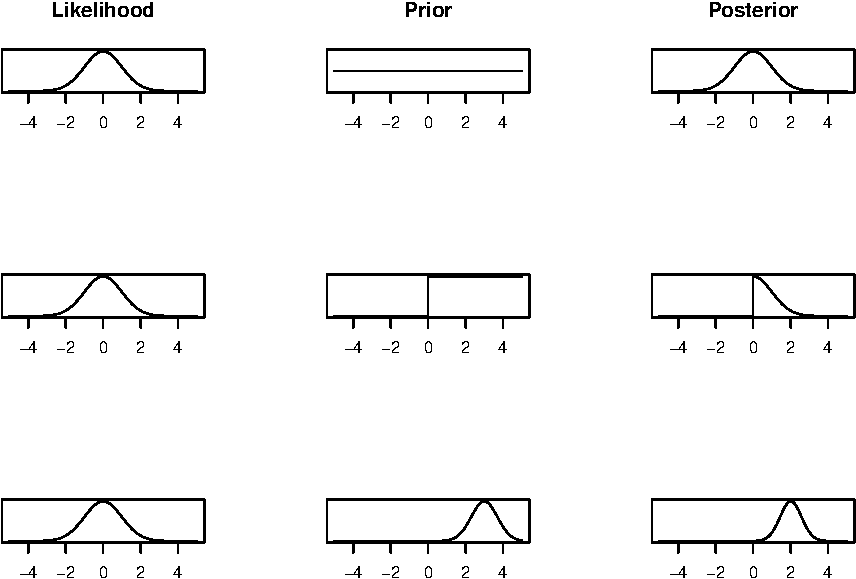
\includegraphics{_main_files/figure-latex/prior-posterior-grid-1.pdf}

\begin{enumerate}
\def\labelenumi{\arabic{enumi}.}
\item
  The posterior distribution is proportional to the likelihood function. The prior distribution closely matches frequentist inference. Both the MLE and posterior mean are 0.
\item
  We get a lopsided posterior distribution, that is proportional to the likelihood function for positive values of \(\theta\), but is 0 for negative values of \(\theta\).
\item
  We get some sort of average of the likelihood function and the prior distribution. Had we collected more data, the posterior distribution would have been weighted toward the information from the likelihood function more.
\end{enumerate}

\end{example}

\hypertarget{programming-in-r}{%
\chapter{Programming in R}\label{programming-in-r}}

\hypertarget{random-numbers-for-loops-and-r}{%
\section{Random Numbers, For Loops and R}\label{random-numbers-for-loops-and-r}}

This first computer lab is about getting used to R. The first step is to download R and Rstudio.

\begin{itemize}
\tightlist
\item
  \href{https://www.r-project.org}{Download R}
\item
  \href{https://posit.co/downloads/}{Download RStudio IDE}
\end{itemize}

The easiest way to learn R is by using it to solve problems. The lab contains four exercises and three ways of approaching the exercise (easy, medium and hard). If you're new to R, use the easy approach and copy and paste the code straight into R -- you'll need to fill in a few blanks though. If you've used R before, or a similar programming language, stick to the medium and hard approaches. This is also an exercise in using Google. Googling around a problem of for specific commands can allow you to quickly find examples (most likely on Stack Overflow) with code you can use.

There are three aims of this lab:

\begin{enumerate}
\def\labelenumi{\arabic{enumi}.}
\tightlist
\item
  Getting used to programming in R.
\item
  Generating random numbers in R.
\item
  \href{https://www.w3schools.com/r/r_for_loop.asp}{Creating for loops in R}.
\end{enumerate}

\begin{example}
Computationally verify that the Poisson distribution with rate \(\lambda = 100\) can be approximated by a normal distribution with mean and variance 100.

To do this, we can generate lots of samples from a Poisson(100) distribution and plot them on top of the density function of the normal distribution with mean and variance 100.

R has four built-in functions for working with distributions. They take the form \texttt{rdist}, \texttt{ddist}, \texttt{pdist}, and \texttt{qdist}. You replace the \texttt{dist} part with the name of the distribution you want to work with, for example \texttt{unif} for the uniform distribution or \texttt{norm} for the normal distribution. As we are working with the the Poisson distribution, we will use \texttt{pois}. The prefixes allow you to work with the distribution in different ways: \texttt{r} gives you random numbers sampled form the distribution, \texttt{d} evaluates the density function, \texttt{p} evaluates the density function, and \texttt{q} evaluates the inverse density function (or quantile function).

The function \texttt{rpois} allows us to generate samples from a Poisson distribution. We store 10,000 samples in a vector \texttt{y} by calling

\begin{Shaded}
\begin{Highlighting}[]
\NormalTok{y }\OtherTok{\textless{}{-}} \FunctionTok{rpois}\NormalTok{(}\AttributeTok{n =} \DecValTok{10000}\NormalTok{, }\AttributeTok{lambda =} \DecValTok{100}\NormalTok{)}
\end{Highlighting}
\end{Shaded}

We can generate a histogram of \texttt{y} using the \texttt{hist} command. Setting \texttt{freq\ =\ FALSE}, makes R plot a density histogram instead of a frequency histogram. Typing \texttt{?hist} will give you more information about this

\begin{Shaded}
\begin{Highlighting}[]
\FunctionTok{hist}\NormalTok{(y, }\AttributeTok{freq =} \ConstantTok{FALSE}\NormalTok{, }\AttributeTok{xlab =} \StringTok{"y"}\NormalTok{, }\AttributeTok{main =} \StringTok{""}\NormalTok{)}
\end{Highlighting}
\end{Shaded}

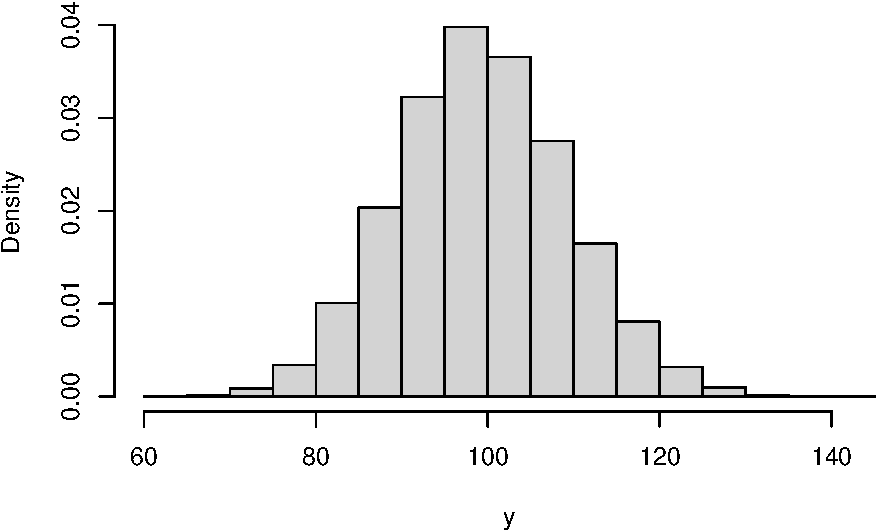
\includegraphics{_main_files/figure-latex/unnamed-chunk-3-1.pdf}

The last thing to do is to plot the normal density on top. There are a couple of ways of doing this. The way below generates a uniform grid of points and then evaluates the density at each point. Finally, it adds a line graph of these densities on top.

\begin{Shaded}
\begin{Highlighting}[]
\NormalTok{x }\OtherTok{\textless{}{-}} \FunctionTok{seq}\NormalTok{(}\AttributeTok{from =} \DecValTok{50}\NormalTok{, }\AttributeTok{to =} \DecValTok{150}\NormalTok{, }\AttributeTok{by =} \DecValTok{1}\NormalTok{)           }\CommentTok{\#create uniform grid on [50, 150]}
\NormalTok{density }\OtherTok{\textless{}{-}} \FunctionTok{dnorm}\NormalTok{(x, }\AttributeTok{mean =} \DecValTok{100}\NormalTok{, }\AttributeTok{sd =} \FunctionTok{sqrt}\NormalTok{(}\DecValTok{100}\NormalTok{)) }\CommentTok{\#compute density}

\CommentTok{\#plot together}
\FunctionTok{hist}\NormalTok{(y, }\AttributeTok{freq =} \ConstantTok{FALSE}\NormalTok{, }\AttributeTok{xlab =} \StringTok{"y"}\NormalTok{, }\AttributeTok{main =} \StringTok{""}\NormalTok{)}
\FunctionTok{lines}\NormalTok{(x, density)}
\end{Highlighting}
\end{Shaded}

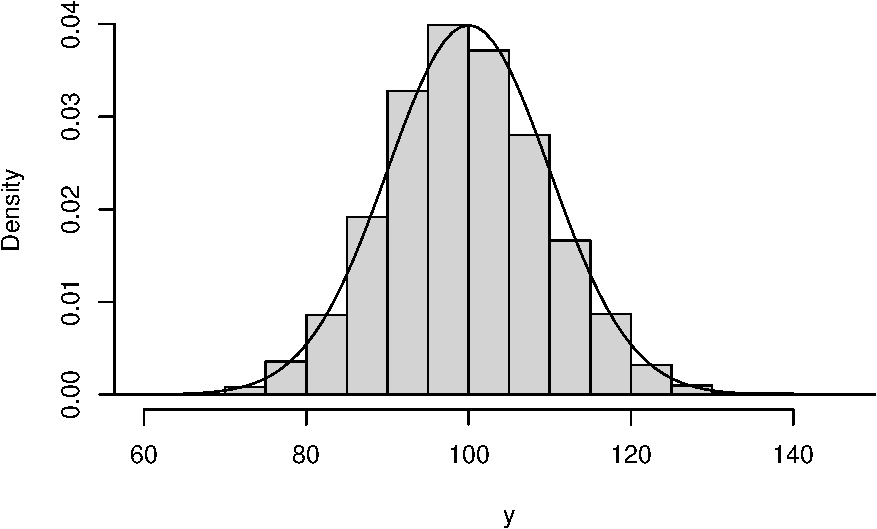
\includegraphics{_main_files/figure-latex/unnamed-chunk-4-1.pdf}

The two match up well, showing the normal distribution is a suitable approximation here.
\end{example}

Over the next two sessions, you will need to solve the following four problems in R. You can type \texttt{?} before any function in R (e.g.~\texttt{?rnorm}) to bring up R's helpage on the function. Googling can also bring up lots of information, possible solutions and support.

\begin{exercise}

The changes in the Birmingham stock exchange each day can be modelled using a normal distribution. The price on day \(i\), \(X_i\) is given by
\[
X_i = \alpha X_{i-1}, \qquad \alpha \sim N(1.001, 0.005^2).
\]
The index begins at \(X_0 = 100\). Investigate the distribution of the value of the stock market on days 50 and 100.

\textbf{Hard}. Use a simulation method to generate the relevant distributions.

\textbf{Medium}. Simulate the value for \(\alpha\) for each of the 100 days and use the \texttt{cumprod} command to plot a trajectory. Use a for loop to repeat this 100 times and investigate the distribution of the value of the stock market on days 50 and 100.

\textbf{Easy}. Fill in the blanks in the following code.

\begin{verbatim}
# Plot one ----------------------------------------------------------------
x <- rnorm(n = , mean = , sd = ) #Simulate daily change for 100 days
plot(, type = 'l') #multiply each day by the previous days

# Plot 100 realisations ---------------------------------------------------
market.index <- matrix(NA, 100, 100) #Initialise a matrix to store trajectories
for(i in 1:100){
  x <- rnorm(n = , mean = , sd = )
  market.index [, i] <- 
}

#Plot all trajectories
matplot(market.index, type = 'l')

#Get distribution of days 50 and 100
hist()
hist()
quantile(, )
quantile(, )
\end{verbatim}

\end{exercise}

\begin{exercise}

You are an avid lottery player and play the lottery twice a week, every week for 50 years (a total of 5,200 times). The lottery has 50 balls labeled 1, \ldots, 50 and you play the same 6 numbers each time. Six out of the 50 balls are chosen uniformly at random and the prize money is shown in the table below.

\begin{longtable}[]{@{}ll@{}}
\toprule\noalign{}
Numbers Matched & Prize Amount \\
\midrule\noalign{}
\endhead
\bottomrule\noalign{}
\endlastfoot
0-2 & £0 \\
3 & £30 \\
4 & £140 \\
5 & £1,750 \\
6 & £1,000,000 \\
\end{longtable}

It costs you £2 to play each time. Simulate one set of 5,200 draws. How much do you win? What is your total profit/loss?

\textbf{Hard}. Use a for loop and sequence of if else statements to generate your prize winnings.

\textbf{Medium}. Use a for loop to generate the lottery numbers and prize winnings for each draw. Use the \texttt{sample} function to generate a set of lottery numbers and check they match against your numbers using the \texttt{\%in\%} function. Finally, use if else statements to check how much you have won each time.

\textbf{Easy}. Fill in the blanks in the following code.

\begin{verbatim}
my.numbers <- 

#For loop to generate lottery numbers and prize winnings
prize <- numeric(5200)
for(i in 1:5200){
  
  #Generate lottery numbers
  draw <- sample(, )
  
  #Check how many match my numbers
  numbers.matched <- #use %in% function
  
  #Compute prize winings
  if(numbers.matched < 3)
    prize[i] <- 0
  else if()
    prize[i] <-  30
  else if()
    prize[i] <-  140
  else if()
    prize[i] <-  1750
  else
    prize[i] <- 1000000
}

#Summarise prize winnings
table(prize)
hist(prize)
sum(prize) - 2*5200
\end{verbatim}

\end{exercise}

\begin{exercise}
Estimate \(\pi\).

\textbf{Hard}. Use a rejection sampling algorithm.

\textbf{Medium}. Generate lots of points \((x, y)\) on the unit square \([0, 1]^2\). Check each point to see if it lies within the unit circle. Use the proportion of points that lie within the unit circle to estimate \(\pi\).

\textbf{Easy}. Fill in the blanks in the following code.

\begin{verbatim}
#Sample on unit square
N <- 10000      #number of points
x <-            #sample N points uniformly at random on [0, 1]
y <-            #sample N points uniformly at random on [0, 1]

#Estimate pi
r.sq                 <- x^2 + y^2                #check how far from origin
number.inside.circle <-           #count how many points inside unit cirlce
pi.estimate          <- 

#Plot points
par(pty = "s")         #make sure plot is square
plot(x, y, cex = 0.1)  #plot points
theta <- seq(0, pi/2, 0.01) #plot unit circle
lines(x = cos(theta), y = sin(theta), col = "red")
\end{verbatim}

\textbf{Extra}. Use a for loop to repeat this for \(N = \{1, \ldots, 10000\}\). Record the estimate for \(\pi\) for each value and the relative error.
\end{exercise}

\begin{exercise}

A linear congruential generator (LCG) is a simple algorithm for generating random integers. Given a starting value \(X_0\), it generates a sequence of integers according to
\[
X_{i+1} = a X_i + c \mod m.
\]
Software that generates numbers using an LCG Setting \(a = 3\), \(c = 2\), \(m = 7\) and \(X_0 = 0\), generate 20 samples from this generator.

\begin{enumerate}
\def\labelenumi{\arabic{enumi}.}
\item
  Investigate the `randomness' of this generator by creating the delay plot, where \(X_{i-1}\) is plotted against \(X_{i}\)
\item
  One way to improve the quality of these generators is to shuffle the sequence generated. Generate rate two sequences \(X\) and \(Y\) from two different LCGs, and report the shuffled sequence \(Z_j = X_{Y_j}\). For the sequence \(Y\) use the values \(a = 5\), \(c = 1\), \(m = 8\) and \(Y_0 = 2\).
\item
  As the past two exercises show, LCGs are notoriously poor. in the 1960s and 70s, RANDU was a widely used LCG developed by IBM. According to Wikipedia
  \textgreater{} IBM's RANDU is widely considered to be one of the most ill-conceived random number generators ever designed, and was described as ``truly horrible'' by Donald Knuth.
\end{enumerate}

The RANDU LCG uses \(a = 2^{16} + 3\), \(c = 0\), \(m = 2^{31}\) and \(Y_0 = 1\). Generate a sequence of 10,000 pseudorandom variables from the RANDU LCG and create the delay plot.

The delay plot seems to show little relationship between \(X_{i}\) and \(X_{i+1}\). The third order delay plot is a 3d-plot with coordinate \((X_i, X_{i+1}, X_{i+2})\) and this plot shows a different picture. Create this plot using the code

\begin{verbatim}
#install.packages("scatterplot3d") #you may need to install this package
scatterplot3d::scatterplot3d(X[1:9998], X[2:9999], X[3:10000], angle=154, 
                             xlab = expression(X[i]), ylab = expression(X[i+1]), zlab = expression(X[i+2]))
\end{verbatim}

This is what makes the RANDU LCG so poor. Write down \(X_{i+1}\) and \(X_{i+2}\) in terms of \(X_i\). Show that \(X_{i+2} = \alpha X_{i+1} + \beta X_{i}\).

\textbf{Hard}. Use a for loop to construct sequences from the LCGs \(X\) and \(Y\).

\textbf{Medium}. Create a for loop to generate the value for the sequence \(X_i\) for \(i = 1, \ldots, 20\). Modular arithmetic can be performed using the \texttt{\%\%} function. Create a new for loop to construct the sequence \(Y\). To shuffle the sequence \(X\) using \(Y\), you will need to subset \(X\) by \(Y\) in R.

\textbf{Easy}. Fill in the blanks in the code below

\begin{verbatim}
# 1. Shuffling ---------------------------------------------------------------
X <- numeric(21) #initialise vector to store X

#Set values for LCG
a <- 
c <- 
m <- 
X[1]<- 


#Run Generator
for(i in 2:21){
  X[i] <-
}
X

#Delay plot
plot( , , xlab = expression(X[i-1]), ylab = expression(X[i]), type = 'l')



# 2. Shuffling ---------------------------------------------------------------

Y <- numeric(21) #initialise vector to store Y

#Set values for LCG
a <- 
c <- 
m <- 
Y[1]<- 


#Run Generator
for(i in 2:50){
  Y[i] <- 
}

#report sequence
Y
X[Y]

#Plot delay plot
plot(x = ,y = , xlab = expression(Z[i-1]), ylab = expression(Z[i]), type = 'l')
\end{verbatim}

\end{exercise}

\hypertarget{functions-in-r}{%
\section{Functions in R}\label{functions-in-r}}

The purpose of this lab is to learn how to write functions is R. Functions are wrappers that allow you to easily repeat commands, as well as customise specific pieces of code.

\hypertarget{built-in-commands}{%
\subsection{Built in commands}\label{built-in-commands}}

R has many build in commands and you used these in Computer Lab I. An example is the \texttt{runif} command from the second exercise. This function generates random numbers from an interval. The code chunk below shows it in action:

\begin{Shaded}
\begin{Highlighting}[]
\NormalTok{u }\OtherTok{\textless{}{-}} \FunctionTok{runif}\NormalTok{(}\AttributeTok{n =} \DecValTok{10}\NormalTok{, }\AttributeTok{min =} \SpecialCharTok{{-}}\DecValTok{1}\NormalTok{, }\AttributeTok{max =} \DecValTok{1}\NormalTok{)}
\NormalTok{u}
\end{Highlighting}
\end{Shaded}

\begin{verbatim}
##  [1]  0.067087419  0.940651611 -0.584863209 -0.008208485 -0.295150339
##  [6] -0.350848322 -0.999261089  0.627317125  0.040368462 -0.383698324
\end{verbatim}

The functions has three \textbf{arguments}: \emph{n} the number of samples to be generated, \emph{min} the lower limit of the interval, \emph{max} the upper limit of the interval. In the code chunk above 10 random numbers were generated from the interval {[}-1, 1{]}. In R, you don't need to label the arguments, so the following will sample the same number of samples from the same interval:

\begin{verbatim}
u <- runif(10, -1, 1)
\end{verbatim}

Although in most cases it helps to label the arguments for readability and avoiding undefined behaviour. Note that if you decide to omit the argument names in the function call, the arguments must appear exactly in the order defined by the function prototype (check the documentation ?function for specific cases).

\hypertarget{user-defined-functions}{%
\subsection{User defined functions}\label{user-defined-functions}}

In many cases, we will need to repeat the same piece of code over and over again, or we will need to run it again with different values. In this case, we can write our own function. In R, there are two ways to type your own function. The first is to write a full function definition. The basic template is

\begin{verbatim}
name.of.function <- function(arguments){

  #do something
  #produce result
  
  return(result)

}
\end{verbatim}

The second way is an in-line function, which is sometimes useful for short functions. The template is

\begin{verbatim}
name.of.function <- function(arguments) #do something
\end{verbatim}

In this module, we're going to use the full function way of writing functions.

\begin{example}
In this example, we're going to write a function to evaluate the normal density function. The density function is given by
\[
\pi(x \mid \mu, \sigma^2) = \frac{1}{\sqrt{2\pi\sigma^2}}e^{\left\{-\frac{1}{2\sigma^2}(x-\mu)^2\right\}}.
\]

We will need our function to take three arguments, the value at which the density function needs to be evaluated, and the mean and standard deviation of the distribution.

\begin{Shaded}
\begin{Highlighting}[]
\NormalTok{normal.density }\OtherTok{\textless{}{-}} \ControlFlowTok{function}\NormalTok{(x, mu, sigma)\{}
  
\NormalTok{  fraction.term }\OtherTok{\textless{}{-}} \DecValTok{1}\SpecialCharTok{/}\FunctionTok{sqrt}\NormalTok{(}\DecValTok{2}\SpecialCharTok{*}\NormalTok{pi}\SpecialCharTok{*}\NormalTok{sigma}\SpecialCharTok{\^{}}\DecValTok{2}\NormalTok{)}
\NormalTok{  exponent.term }\OtherTok{\textless{}{-}} \SpecialCharTok{{-}}\DecValTok{1}\SpecialCharTok{/}\NormalTok{(}\DecValTok{2}\SpecialCharTok{*}\NormalTok{sigma}\SpecialCharTok{\^{}}\DecValTok{2}\NormalTok{)}\SpecialCharTok{*}\NormalTok{(x}\SpecialCharTok{{-}}\NormalTok{mu)}\SpecialCharTok{\^{}}\DecValTok{2}
  
\NormalTok{  result }\OtherTok{\textless{}{-}}\NormalTok{ fraction.term}\SpecialCharTok{*}\FunctionTok{exp}\NormalTok{(exponent.term)}
  \FunctionTok{return}\NormalTok{(result)}
  
\NormalTok{\}}
\end{Highlighting}
\end{Shaded}

We have split up the density into two parts to make it easier to code up and read. R has its own inbuilt normal density function \texttt{dnorm} and we can compare our function against R's. Although R's is faster and more reliable, we should get the same results.

\begin{Shaded}
\begin{Highlighting}[]
\FunctionTok{normal.density}\NormalTok{(}\AttributeTok{x =} \FloatTok{0.5}\NormalTok{, }\AttributeTok{mu =} \DecValTok{1}\NormalTok{, }\AttributeTok{sigma =} \FloatTok{0.5}\NormalTok{)}
\end{Highlighting}
\end{Shaded}

\begin{verbatim}
## [1] 0.4839414
\end{verbatim}

\begin{Shaded}
\begin{Highlighting}[]
\FunctionTok{dnorm}\NormalTok{(}\AttributeTok{x =} \FloatTok{0.5}\NormalTok{, }\AttributeTok{mean =} \DecValTok{1}\NormalTok{, }\AttributeTok{sd =} \FloatTok{0.5}\NormalTok{)}
\end{Highlighting}
\end{Shaded}

\begin{verbatim}
## [1] 0.4839414
\end{verbatim}

Why might R's function be faster and more reliable than ours?
\end{example}

\begin{exercise}
Write a function to evaluate the log of the probability density function of a Poisson distribution with rate \(\lambda\).
\end{exercise}

\begin{exercise}
Consider the stock exchange problem in Exercise 2.1. Write a function that simulates 100 days of the stock exchange. Use the \texttt{replicate} function to call this function 10,000 times.
\end{exercise}

\hypertarget{good-coding-practices}{%
\section{Good Coding Practices}\label{good-coding-practices}}

In the past two labs, we've written code to solve different problems. In this lab, we're going to take a step back and think about what good R code does and doesn't look like.

\hypertarget{code-style}{%
\subsection{Code Style}\label{code-style}}

Code should be both efficient and easy to read. In most cases it's better to write code that's easy to read and less efficient, than highly efficient code that's difficult to read. Some basic principles to make code easy to read are:

\begin{enumerate}
\def\labelenumi{\arabic{enumi}.}
\tightlist
\item
  Write short functions names, e.g.~\texttt{buy.loot.box} is better than \texttt{player.buys.one.loot.boox} or \texttt{blb}.
\item
  Document and comment code. In R comments start with \texttt{\#}.
\item
  Multiple short functions are better than long functions that do multiple things.
\item
  Be consistent.
\end{enumerate}

\begin{example}
Review the \href{https://style.tidyverse.org/index.html}{tidyverse Style Guide}.
\end{example}

\begin{example}
Review \href{https://google.github.io/styleguide/Rguide.html}{Google's R Style Guide}.
\end{example}

One way to ensure code style is consistent and bug free is to carry out code reviews. These are common both in academia and industry. A code review is where someone else goes through your code line-by-line ensuring it conforms to the company style and doesn't have any bugs.

\begin{exercise}

The following code is for Exercises 2.1 about the stock exchange. Restyle the code so it is easy to read.

\begin{verbatim}
# Plot one ----------------------------------------------------------------
rnorm(100,1.001,0.5) -> x 
plot(100*cumprod(x),type ='l') 
# Plot 100 realisations ---------------------------------------------------
X <- matrix(NA, 100, 100) 
for(i in 1:100){
  x <- rnorm(100, 1.001, 0.005)
  X[,i] <- 100*cumprod(x)
}
matplot(X,type ='l')
hist(X[50,]);hist(X[100,]);quantile(X[50,], c(0.25, 0.5, 0.75));quantile(X[100,], c(0.25, 0.5, 0.75))
\end{verbatim}

\end{exercise}

\begin{exercise}

In pairs or groups, carry out a code review for one of your solutions to an exercise from a previous lab. Remember to

\begin{enumerate}
\def\labelenumi{\arabic{enumi}.}
\tightlist
\item
  Make sure the coding style is consistent.
\item
  Identify any bugs.
\item
  Be respectful and constructive in your feedback.
\end{enumerate}

\end{exercise}

\hypertarget{bayesian-inference}{%
\chapter{Bayesian Inference}\label{bayesian-inference}}

Whereas Chapter 1 dealt with the fundamentals of Bayesian inference and definitions, Chapter 3 is much more practical. We are going to be deriving posterior distributions and proving when it does and doesn't work.

\hypertarget{the-binomial-distribution}{%
\section{The Binomial Distribution}\label{the-binomial-distribution}}

The first example we are going to go through is with the Binomial distribution.

\begin{example}
\protect\hypertarget{exm:binom}{}\label{exm:binom}A social media company wants to determine how many of its users are bots. A software engineer collects a random sample of 200 accounts and finds that three are bots. She uses a Bayesian method to estimate the probability of an account being a bot. She labels the accounts with a 1 if they are a bot and 0 if there is are a real person. The set of account labels is given by \(\boldsymbol{y} = \{y_1, \ldots, y_{200}\}\) and the probability an account is a bot is \(\theta\). By Bayes' theorem, we obtain the following,
\[
\pi(\theta \mid \boldsymbol{y}) \propto \pi(\boldsymbol{y}\mid \theta) \pi(\theta).
\]

\textbf{Likelihood function} \(\pi(\boldsymbol{y}\mid \theta)\). We observe 200 trials each with the same probability of success (denoted by \(\theta\)) and probability of failure (given by \(1-\theta\)). The Binomial distribution seems the most suitable way of modelling this. Therefore, the likelihood function is given by,
\[
\pi(\boldsymbol{y}\mid \theta) = \begin{pmatrix} 200 \\ 3 \end{pmatrix} \theta^3(1-\theta)^{197},
\]
assuming that any two accounts being a bot are independent of one another.

\textbf{Prior distribution} \(\pi(\theta)\). We now need to describe our prior beliefs about \(\theta\). We have no reason to suggest \(\theta\) takes any specific value, so we use a uniform prior distribution \(\theta \sim U[0, 1]\), where \(\pi(\theta) = 1\) for \(\theta \in [0, 1]\).

\textbf{Posterior distribution} \(\pi(\theta \mid \boldsymbol{y})\). We can now derive the posterior distribution up to proportionality
\[
\pi(\theta \mid \boldsymbol{y}) \propto \theta^3(1-\theta)^{197}. 
\]
This functional dependence on \(\theta\) identifies the \(\pi(\theta \mid \boldsymbol{y})\) is a Beta distribution. The PDF for the beta distribution with shape parameters \(\alpha\) and \(\beta\) is
\[
\pi(x \mid \alpha, \beta) = \frac{\Gamma(\alpha + \beta)}{\Gamma(\alpha)\Gamma(\beta)}x^{\alpha - 1}(1-x)^{\beta - 1}. 
\]
The posterior distribution is therefore \(\theta \mid \boldsymbol{y} \sim \textrm{Beta}(4, 198)\).
\end{example}

\hypertarget{reporting-conclsuions-from-bayesian-inference}{%
\section{Reporting Conclsuions from Bayesian Inference}\label{reporting-conclsuions-from-bayesian-inference}}

In the previous example, we derived the posterior distribution \(\theta \mid \boldsymbol{y} \sim \textrm{Beta}(4, 198)\). But often, we want to share more descriptive information about our beliefs given the observed data. In this example, the posterior mean given the data is \(\frac{4}{198} = \frac{2}{99}\). That is to say given the data, we expect that for every 99 accounts, two to be bots. The posterior mode for \(\theta\) is \(\frac{3}{200}\) or 1.5\%.

It is important to share the uncertainty about out beliefs. In a frequentist framework, this would be via a confidence interval. The Bayesian analogues is a credible interval.

\begin{definition}
A \textbf{credible interval} is a central interval of posterior probability which corresponds, in the case of a 100\((1-\alpha)\)\% interval, to the range of values that capture 100\((1-\alpha)\)\% of the posterior probability.
\end{definition}

\begin{example}
The 95\% credible interval for the Binomial example is given by

\begin{Shaded}
\begin{Highlighting}[]
\NormalTok{cred.int}\FloatTok{.95} \OtherTok{\textless{}{-}} \FunctionTok{qbeta}\NormalTok{(}\FunctionTok{c}\NormalTok{(}\FloatTok{0.025}\NormalTok{, }\FloatTok{0.975}\NormalTok{), }\DecValTok{4}\NormalTok{, }\DecValTok{198}\NormalTok{)}
\FunctionTok{round}\NormalTok{(cred.int}\FloatTok{.95}\NormalTok{, }\DecValTok{3}\NormalTok{)}
\end{Highlighting}
\end{Shaded}

\begin{verbatim}
## [1] 0.005 0.043
\end{verbatim}

This says that we believe there is a 95\% chance that the probability of an account being a bot lies between 0.005 and 0.043. This is a much more intuitive definition to the confidence interval, which says if we ran the experiment an infinite number of times and computed an infinite number of confidence intervals, 95\% of them would contain the true value of \(\theta\).
\end{example}

\hypertarget{the-exponential-distribution}{%
\section{The Exponential Distribution}\label{the-exponential-distribution}}

\begin{example}
\protect\hypertarget{exm:exponential}{}\label{exm:exponential}

An insurance company want to estimate the time until a claim is made on a specific policy. They describe the rate at which claims come in by \(\lambda\). The company provides a sample of 10 months at which a claim was made \(\boldsymbol{y} = \{14, 10, 6, 7, 13, 9, 12, 7, 9, 8\}\). By Bayes' theorem, the posterior distribution for \(\lambda\) is
\[
\pi(\lambda \mid \boldsymbol{y}) \propto \pi(\boldsymbol{y} \mid \lambda) \pi(\lambda).
\]

\textbf{Likelihood function} \(\pi(\boldsymbol{y} \mid \lambda)\). The exponential distribution is a good way of modelling lifetimes or the length of time until an event happens. Assuming all the claims are independent of one another, the likelihood function is given by
\begin{align*}
\pi(\boldsymbol{y} \mid \lambda) &= \prod_{i=1}^{10} \lambda e^{-\lambda y_i} \\
& = \lambda^{10}e^{-\lambda \sum_{i=1}^{10} y_i} \\
& = \lambda^{10} e^{-95\lambda}.
\end{align*}

\textbf{Prior distribution} \(\pi(\lambda)\). As we are modelling a rate parameter, we know it must be positive and continuous. We decide to use an exponential prior distribution for \(\lambda\), but leave the choice of the rate parameter up to the insurance professionals at the insurance company. The prior distribution is given by \(\lambda \sim \textrm{Exp}(\gamma).\)

\textbf{Posterior distribution} \(\pi(\lambda \mid \boldsymbol{y})\). We now have all the ingredients to derive the posterior distribution. It is given by
\begin{align*}
\pi(\lambda \mid \boldsymbol{y}) &\propto \lambda^{10} e^{-95\lambda} \times e^{-\gamma\lambda} \\
& \propto \lambda^{10}e^{-(95 + \gamma)\lambda}
\end{align*}
The functional form tells us that the posterior distribution is a Gamma distribution. The PDF of a gamma random variable with shape \(\alpha\) and rate \(\beta\) is
\[
\pi(x \mid \alpha, \beta) = \frac{\alpha^\beta}{\Gamma(\alpha)}x^{\alpha-1}e^{-\beta x}.
\]
The distribution of the rate of the claims given the observed data is \(\lambda \mid \boldsymbol{y} \sim \textrm{Gamma}(11, 95 + \gamma)\).

The posterior mean months until a claim is \(\frac{11}{95 + \gamma}\). We can see the effect of the choice of rate parameter in this mean. Small values of \(\gamma\) yield vague prior distribution, which plays a minimal role in the posterior distribution. Large values of \(\gamma\) result in prior distributions that contribute a lot to the posterior distribution. The plots below show the prior and posterior distributions for \(\gamma = 0.01\) and \(\gamma = 50\).

\begin{Shaded}
\begin{Highlighting}[]
\NormalTok{plot.distributions }\OtherTok{\textless{}{-}} \ControlFlowTok{function}\NormalTok{(gamma.prior)\{}
  \CommentTok{\#evaluate at selected values of lambda}
\NormalTok{  lambda }\OtherTok{\textless{}{-}} \FunctionTok{seq}\NormalTok{(}\FloatTok{0.001}\NormalTok{, }\FloatTok{0.3}\NormalTok{, }\FloatTok{0.001}\NormalTok{) }
  
  \CommentTok{\#evaluate prior density}
\NormalTok{  prior }\OtherTok{\textless{}{-}} \FunctionTok{dexp}\NormalTok{(lambda, }\AttributeTok{rate =}\NormalTok{ gamma.prior)}
  
  \CommentTok{\#evaluate posterior density}
\NormalTok{  posterior }\OtherTok{\textless{}{-}} \FunctionTok{dgamma}\NormalTok{(lambda, }\AttributeTok{shape =} \DecValTok{11}\NormalTok{, }\AttributeTok{rate =} \DecValTok{95} \SpecialCharTok{+}\NormalTok{ gamma.prior)}
  
  
  \CommentTok{\#plot}
  \FunctionTok{plot}\NormalTok{(lambda, posterior, }\AttributeTok{type=} \StringTok{\textquotesingle{}l\textquotesingle{}}\NormalTok{, }
       \AttributeTok{ylim =} \FunctionTok{c}\NormalTok{(}\DecValTok{0}\NormalTok{, }\DecValTok{50}\NormalTok{), }\AttributeTok{xlab =} \FunctionTok{expression}\NormalTok{(lambda), }\AttributeTok{ylab =} \StringTok{"density"}\NormalTok{)}
  \FunctionTok{lines}\NormalTok{(lambda, prior, }\AttributeTok{lty =} \DecValTok{2}\NormalTok{)}
  \FunctionTok{legend}\NormalTok{(}\StringTok{\textquotesingle{}topright\textquotesingle{}}\NormalTok{, }\AttributeTok{lty =} \FunctionTok{c}\NormalTok{(}\DecValTok{1}\NormalTok{, }\DecValTok{2}\NormalTok{), }\AttributeTok{legend =} \FunctionTok{c}\NormalTok{(}\StringTok{"Posterior"}\NormalTok{, }\StringTok{"Prior"}\NormalTok{),  }
         \AttributeTok{bty =} \StringTok{"n"}\NormalTok{)}
\NormalTok{\}}

\FunctionTok{plot.distributions}\NormalTok{(}\FloatTok{0.01}\NormalTok{)}
\end{Highlighting}
\end{Shaded}

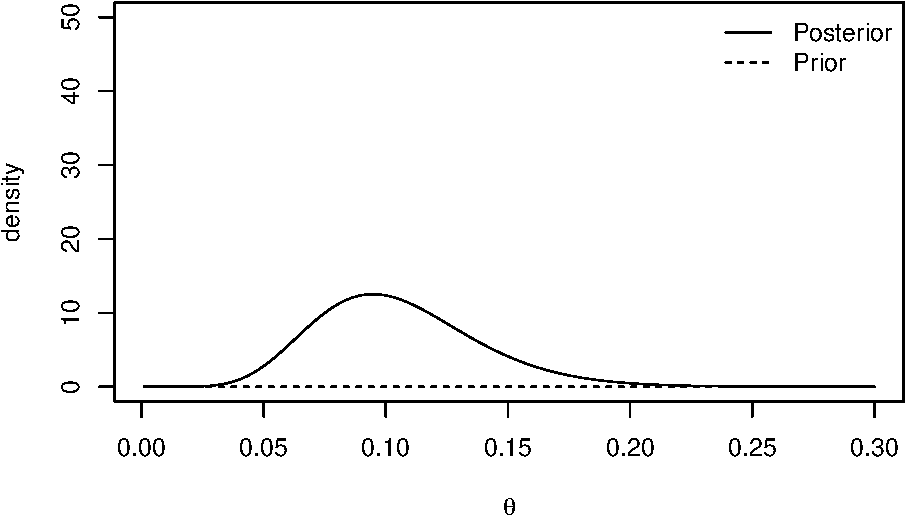
\includegraphics{_main_files/figure-latex/unnamed-chunk-9-1.pdf}

\begin{Shaded}
\begin{Highlighting}[]
\FunctionTok{plot.distributions}\NormalTok{(}\DecValTok{50}\NormalTok{)}
\end{Highlighting}
\end{Shaded}

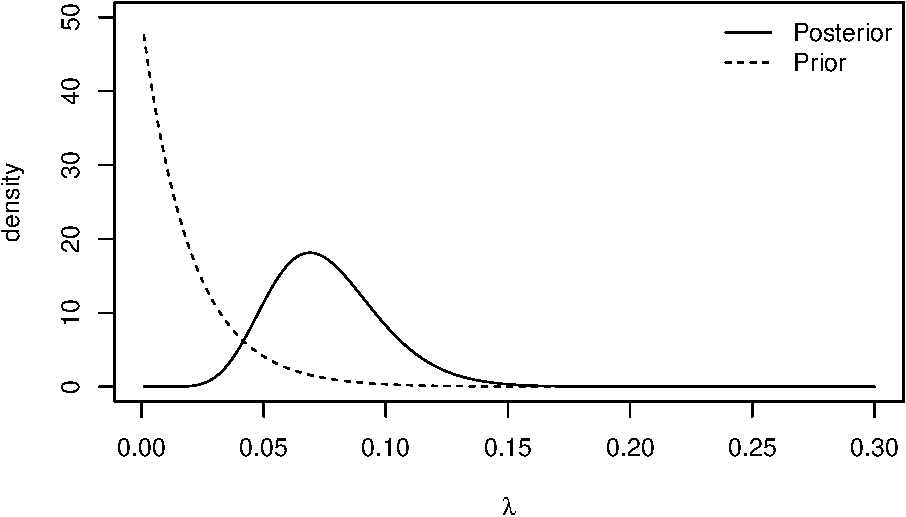
\includegraphics{_main_files/figure-latex/unnamed-chunk-9-2.pdf}

The insurance managers recommend that because this is a new premium, a vague prior distribution be used and \(\gamma = 0.01\). The posterior mean is \(\frac{11}{95.01} \approx 0.116\) and the 95\% credible interval is

\begin{Shaded}
\begin{Highlighting}[]
\FunctionTok{round}\NormalTok{(}\FunctionTok{qgamma}\NormalTok{(}\FunctionTok{c}\NormalTok{(}\FloatTok{0.025}\NormalTok{, }\FloatTok{0.975}\NormalTok{), }\DecValTok{11}\NormalTok{, }\FloatTok{95.01}\NormalTok{), }\DecValTok{3}\NormalTok{)}
\end{Highlighting}
\end{Shaded}

\begin{verbatim}
## [1] 0.058 0.194
\end{verbatim}

\end{example}

\hypertarget{the-normal-distribtuion}{%
\section{The Normal Distribtuion}\label{the-normal-distribtuion}}

The Normal distribution is incredibly useful for modelling a wide range of natural phenomena and in its own right. We're now going to derive posterior distributions for the normal distribution. As we're going to see, the concepts behind deriving posterior distributions are the same as in the previous two examples. However, the algebraic accounting is a lot more taxing.

\begin{example}
\protect\hypertarget{exm:normal}{}\label{exm:normal}

Suppose we observe \(N\) data points \(\boldsymbol{y} = \{y_1, \ldots, y_N\}\) and we assume \(y_i \sim N(\mu, \sigma^2)\) and each observation is independent. Suppose that, somehow, we know the population standard deviation and we wish to estimate the population mean \(\mu\). By Bayes' theorem, the posterior distribution is
\[
\pi(\mu \mid \boldsymbol{y}, \sigma^2) \propto \pi(\boldsymbol{y} \mid \mu, \sigma^2) \pi(\mu)
\]

\textbf{Likelihood function}.
As the observations are independent, the likelihood function is given by the product of the \(N\) normal density functions as follows,
\begin{align*}
\pi(\boldsymbol{y} \mid \mu, \theta^2) &= \prod_{i=1}^{N} \frac{1}{\sqrt{2\pi\sigma^2}}\exp\left\{-\frac{(y_i - \mu)^2}{2\sigma^2}\right\} \\
&= (2\pi\sigma^2)^{-\frac{N}{2}}\exp\left\{-\sum_{i=1}^{N}\frac{(y_i - \mu)^2}{2\sigma^2}\right\}.
\end{align*}

\textbf{Prior distribution} We suppose we have no prior beliefs about the values that \(\mu\) can take. We assign a normal prior distribution to \(\mu \sim N(\mu_0, \sigma_0^2)\) despite it being a time. We will set \(\mu = 0\) and \(\sigma_0^2 = 1000\) to signify our vague prior beliefs, but, for ease, we will use the symbolic values during the derivation of the posterior distribution. We have
\[
\pi(\mu) = \frac{1}{\sqrt{2\pi\sigma_0^2}}\exp\left\{-\frac{1}{2\sigma_0^2}(\mu - \mu_0)^2\right\}.
\]

\textbf{Posterior distribution}. To derive the posterior distribution, up to proportionality, we multiply the prior distribution by the likelihood function. As the fractions out the front of both terms do not depend on \(\mu\), we can ignore these.
\begin{align*}
\pi(\mu \mid \boldsymbol{y}, \sigma^2) &\propto\exp\left\{-\sum_{i=1}^{N}\frac{(y_i - \mu)^2}{2\sigma^2}\right\}  \exp\left\{\frac{1}{2\sigma_0^2}(\mu - \mu_0)^2\right\} \\
& = \exp\left\{-\sum_{i=1}^{N}\frac{(y_i - \mu)^2}{2\sigma^2}-\frac{1}{2\sigma_0^2}(\mu - \mu_0)^2\right\} \\
& = \exp\left\{-\frac{\sum_{i=1}^{N}y_i^2}{2\sigma^2} + \frac{\mu\sum_{i=1}^{N}y_i}{\sigma^2} - \frac{N\mu^2}{2\sigma^2} - \frac{\mu^2}{2\sigma_0^2} + \frac{\mu\mu_0}{\sigma_0^2} - \frac{\mu_0^2}{2\sigma_0^2}\right\}.
\end{align*}

We can drop the first and last term as they do not depend on \(\mu\). With some arranging, the equation becomes
\[
\pi(\mu \mid \boldsymbol{y}, \sigma^2) \propto \exp\left\{-\mu^2\left(\frac{N}{2\sigma^2}  + \frac{1}{2\sigma_0^2}\right) + \mu\left(\frac{\sum_{i=1}^{N}y_i}{\sigma^2} + \frac{\mu_0}{\sigma_0^2} \right)  \right\}
\]
Defining \(\mu_1 =\left(\frac{\sum_{i=1}^{N}y_i}{\sigma^2} + \frac{\mu_0}{\sigma_0^2} \right)\) and \(\sigma^2_1 = \left(\frac{N}{\sigma^2} + \frac{1}{\sigma_0^2}\right)^{-1}\) tidies this up and gives
\[
\pi(\mu \mid \boldsymbol{y}, \sigma^2) \propto \exp\left\{-\frac{\mu^2}{2\sigma_1^2} + \mu\mu_1 \right\}.
\]
Our last step to turning this into a distribution is completing the square. Consider the exponent term, completing the square becomes
\[
-2\sigma_1^2\mu^2 + \mu\mu_1 = -\frac{1}{2\sigma^2_1}\left(\mu - \frac{\mu_1}{\sigma_1^2} \right)^2.
\]
Therefore, the posterior distribution, up to proportionality, is given by
\[
\pi(\mu \mid \boldsymbol{y}, \sigma^2) \propto \exp\left\{-\frac{1}{2\sigma^2_1}\left(\mu - \frac{\mu_1}{\sigma_1^2} \right)^2\right\},
\]
and so the posterior distribution of \(\mu\) is \(\mu \mid \boldsymbol{y}, \sigma^2 \sim N(\mu_1, \sigma^2_1)\).

It may help to consider the meaning of \(\mu_1\) and \(\sigma^2_1\). The variance of the posterior distribution can be thought of as the weighted average of the population and sample precision, where the weight is the number of data points collected. The interpretation of the posterior mean can be seen more easily by writing is as
\[
\mu  = \sigma_1^2\left(\frac{N\bar{y}}{\sigma^2} + \frac{\mu_0}{\sigma_0^2} \right).
\]
The posterior mean is partially defined through the weighted average of the population and prior means, where the weighting depends on the number of data points collected and how precise the distributions are.

Now we have derived the posterior distribution, we can explore it using R. We simulate some data with \(N = 30\), \(\mu = 5\) and \(\sigma^2 = 1\).

\begin{Shaded}
\begin{Highlighting}[]
\CommentTok{\#data}
\NormalTok{N }\OtherTok{\textless{}{-}} \DecValTok{30}
\NormalTok{sigma }\OtherTok{\textless{}{-}} \DecValTok{1}
\NormalTok{y }\OtherTok{\textless{}{-}} \FunctionTok{rnorm}\NormalTok{(N, }\DecValTok{5}\NormalTok{, sigma)}

\CommentTok{\#prior}
\NormalTok{sigma0 }\OtherTok{\textless{}{-}} \DecValTok{1000}
\NormalTok{mu0     }\OtherTok{\textless{}{-}} \DecValTok{0}

\CommentTok{\#posterior}
\NormalTok{sigma1.sq }\OtherTok{\textless{}{-}}\NormalTok{ (}\DecValTok{1}\SpecialCharTok{/}\NormalTok{(sigma0}\SpecialCharTok{\^{}}\DecValTok{2}\NormalTok{)  }\SpecialCharTok{+}\NormalTok{ N}\SpecialCharTok{/}\NormalTok{(sigma}\SpecialCharTok{\^{}}\DecValTok{2}\NormalTok{))}\SpecialCharTok{\^{}{-}}\DecValTok{1}
\NormalTok{mu1       }\OtherTok{\textless{}{-}}\NormalTok{ sigma1.sq}\SpecialCharTok{*}\NormalTok{(}\FunctionTok{sum}\NormalTok{(y)}\SpecialCharTok{/}\NormalTok{(sigma}\SpecialCharTok{\^{}}\DecValTok{2}\NormalTok{) }\SpecialCharTok{+}\NormalTok{ mu0}\SpecialCharTok{/}\NormalTok{(sigma0}\SpecialCharTok{\^{}}\DecValTok{2}\NormalTok{))}

\FunctionTok{c}\NormalTok{(mu1, sigma1.sq) }\CommentTok{\#output mean and variance}
\end{Highlighting}
\end{Shaded}

\begin{verbatim}
## [1] 4.85670749 0.03333333
\end{verbatim}

\begin{Shaded}
\begin{Highlighting}[]
\CommentTok{\#Create plot}
\NormalTok{mu }\OtherTok{\textless{}{-}} \FunctionTok{seq}\NormalTok{(}\DecValTok{4}\NormalTok{, }\DecValTok{6}\NormalTok{, }\FloatTok{0.01}\NormalTok{)}
\NormalTok{posterior }\OtherTok{\textless{}{-}} \FunctionTok{dnorm}\NormalTok{(mu, }\AttributeTok{mean =}\NormalTok{ mu1, }\AttributeTok{sd =} \FunctionTok{sqrt}\NormalTok{(sigma1.sq))}
\FunctionTok{plot}\NormalTok{(mu, posterior, }\AttributeTok{type =}\StringTok{\textquotesingle{}l\textquotesingle{}}\NormalTok{)}
\end{Highlighting}
\end{Shaded}

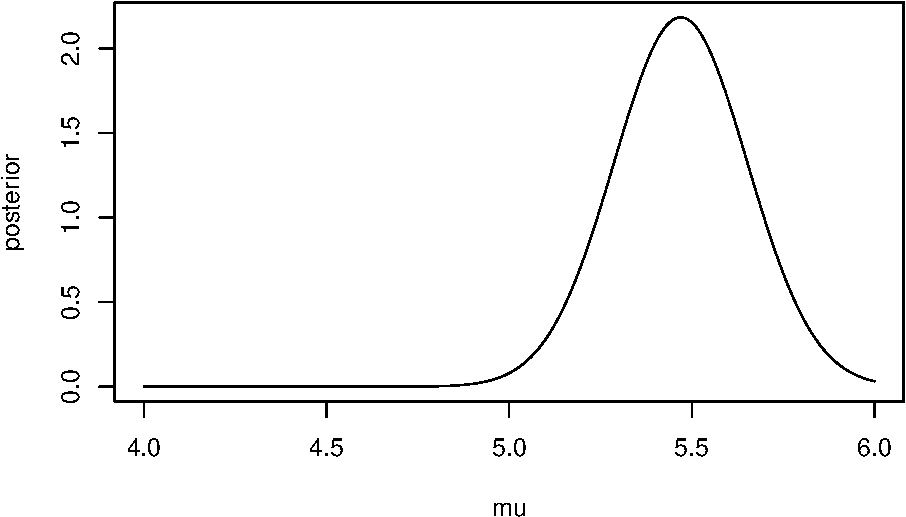
\includegraphics{_main_files/figure-latex/unnamed-chunk-11-1.pdf}

The 95\% credible interval for the population's mean reaction time is

\begin{Shaded}
\begin{Highlighting}[]
\FunctionTok{qnorm}\NormalTok{(}\FunctionTok{c}\NormalTok{(}\FloatTok{0.025}\NormalTok{, }\FloatTok{0.975}\NormalTok{), mu1, }\FunctionTok{sqrt}\NormalTok{(sigma1.sq))}
\end{Highlighting}
\end{Shaded}

\begin{verbatim}
## [1] 4.498869 5.214546
\end{verbatim}

\end{example}

When the prior distribution induces the same function form in the posterior distribution, this is known as conjugacy.

\begin{definition}
If the prior distribution \(\pi(\theta)\) has the same distributional family as the posterior distribution \(\pi(\theta \mid \boldsymbol{y})\), then the prior distribution is a \textbf{conjugate prior distribution}.
\end{definition}

\hypertarget{hierarchical-models}{%
\section{Hierarchical Models}\label{hierarchical-models}}

In many modelling problems, there will be multiple parameters each related to one another. These parameters may be directly related to the model, or they may be parameters we introduce through prior distributions. We can form a hierarchy of these parameters, from closest to further from the data, to construct our model.

\begin{example}
Let's consider \ref{exm:exponential} again. We have some data \(\boldsymbol{y}\) that are assumed to have been generated from an Exponential distribution with rate parameter \(\lambda\). We placed an Exponential prior distribution with rate \(\gamma\) on \(\lambda\) and the posterior distribution was \(\lambda \mid \boldsymbol{y} \sim \textrm{Gamma}(11, 95 + \gamma)\).

In that example, we discussed how the choice of \(\gamma\) can affect the posterior distribution and conclusions presented to the company. One option is to place a prior distribution on \(\gamma\) -- a hyperprior distribution. The hierachy formed is
\begin{align*}
\boldsymbol{y} \mid \lambda &\sim \hbox{Exp}(\lambda) & \textrm{(likelihood)} \\
\lambda \mid \gamma &\sim \hbox{Exp}(\gamma) & \textrm{(prior distribution)} \\
\gamma \mid \nu &\sim \hbox{Exp}(\nu) & \textrm{(hyperprior distribution)}  \\
\end{align*}.
By Bayes' theorem, we can write the posterior distribution as
\begin{align*}
\pi(\lambda, \gamma \mid \boldsymbol{y}) \propto \pi(\boldsymbol{y} \mid \lambda)\pi(\lambda \mid \gamma)\pi(\gamma)\\
&\propto \lambda^{10}e^{-\lambda(95 + \gamma)}\nu e^{-\nu\gamma}.
\end{align*}

To derive the full conditional distributions, we only consider the terms that depends on the parameters we are interested in. The full conditional distribution for \(\lambda\) is
\[
\pi(\lambda \mid \boldsymbol{y}, \,\gamma) \propto \lambda^{10}e^{-\lambda(95 + \gamma)}.
\]
This is unchanged and shows that \(\lambda \mid \boldsymbol{y}, \gamma \sim \textrm{Gamma}(11, 95 + \gamma)\). The full conditional distribution for \(\gamma\) is
\[
\pi(\gamma \mid \boldsymbol{y}, \,\lambda) \propto e^{-\nu\gamma}.
\]
Therefore the full conditional distribution of \(\gamma\) is \(\gamma \mid \boldsymbol{y}, \,\lambda \sim \hbox{Exp}(\lambda + \nu)\).
In the next chapter, we will look at how to sample from these distributions.
\end{example}

\hypertarget{prediction}{%
\section{Prediction}\label{prediction}}

In many cases, although we are interested in drawing inference for the model parameters, what we may also be interested in is predicting new values, whose distribution is determined by the model parameters and observed data.

\begin{definition}
Suppose we observe some data \(\boldsymbol{y}\) given some model parameters \(\theta\) and assign a prior distribution to \(\theta\) and hence derive the posterior distribution \(\pi(\theta \mid \boldsymbol{y})\). The quantity we are interested in is some future observation \(z\), we would like to the distribution of \(z\) given the observed data \(\boldsymbol{y}\), denoted by \(\pi(z \mid \boldsymbol{y})\). This distribution, known as the \textbf{posterior predictive distribution} of \(z\) must be exhibited as a mixture distribution over the possible values of \(\theta\) and is written as,
\[
\pi(z \mid \boldsymbol{y}) = \int \pi(z \mid \theta) \pi(\theta \mid \boldsymbol{y})\, d\theta.
\]
\end{definition}

\begin{example}

Students have to submit coursework for a particular statistical modules. However, each semester a number of students miss the deadline and hand in their coursework late. Last year, three out of 20 students handed their coursework in late. This year, the course has thirty students in. How many students can we expect to hand in their coursework late?

We can model the number of students handing their coursework in late, denoted by \(Y\), using a Binomial distribution, i.e.~\(Y \sim \textrm{Bin}(n, \theta)\) where \(n\) is the number of students and \(\theta\) is the probability of any particular student handing in their coursework late. As in Example \ref{exm:binom}, we assign a uniform prior distribution to \(\theta \sim U[0, 1]\). Given then observed data, we can derive \(\theta \mid \boldsymbol{y} \sim Beta(4, 28)\) (See problem sheets for derivation).

Now we can derive the posterior predictive distribution of \(Z\), the number of students who hand in late. We model \(Z\) using a Binomial distribution, \(Z \sim \textrm{Bin}(30, \theta)\). The distribution of \(Z\) given the observed data is

\begin{align*}
\pi(z \mid \boldsymbol{y}) &= \int_0^1 \pi(z \mid \theta) \pi(\theta \mid \boldsymbol{y})\, d\theta \\
& = \int_0^1 \begin{pmatrix} 30 \\ z \end{pmatrix} \theta^z (1-\theta)^{30 - z} \frac{\Gamma(32)}{\Gamma(4)\Gamma(28)}\theta^{3}(1-\theta)^{27}\, d\theta \\
 & = \begin{pmatrix} 30 \\ z \end{pmatrix}\frac{\Gamma(32)}{\Gamma(4)\Gamma(28)}\int_0^1 \theta^{z + 3}(1-\theta)^{57 - z}\, d\theta \\
\end{align*}
This integral is difficult to evaluate immediately. But by multiplying (and dividing outside the integral) by a constant, we can turn it into the density function of a Beta\((5 + z, 58 - z)\) random variable. This integrates to 1.

\begin{align*}
\pi(z \mid \boldsymbol{y})  & = \begin{pmatrix} 30 \\ z \end{pmatrix}\frac{\Gamma(32)}{\Gamma(4)\Gamma(28)}\frac{\Gamma(z+4)\Gamma(58-z)}{\Gamma(62)}\int_0^1 \frac{\Gamma(62)}{\Gamma(z+4)\Gamma(58-z)}\theta^{z + 3}(1-\theta)^{57 - z}\, d\theta \\ 
& = \begin{pmatrix} 30 \\ z \end{pmatrix}\frac{\Gamma(32)\Gamma(z+4)\Gamma(58-z)}{\Gamma(4)\Gamma(28)\Gamma(62)} \quad \textrm{for }  z \in \{0,1,...,30 \}.
\end{align*}

This code implements the distribution

\begin{Shaded}
\begin{Highlighting}[]
\NormalTok{beta.binom.posterior.predictive.distribution }\OtherTok{\textless{}{-}} \ControlFlowTok{function}\NormalTok{(z)\{}
  
  
\NormalTok{  numerator }\OtherTok{\textless{}{-}} \FunctionTok{gamma}\NormalTok{(}\DecValTok{32}\NormalTok{)}\SpecialCharTok{*}\FunctionTok{gamma}\NormalTok{(z }\SpecialCharTok{+} \DecValTok{4}\NormalTok{)}\SpecialCharTok{*}\FunctionTok{gamma}\NormalTok{(}\DecValTok{58}\SpecialCharTok{{-}}\NormalTok{z)}
\NormalTok{  denominator }\OtherTok{\textless{}{-}} \FunctionTok{gamma}\NormalTok{(}\DecValTok{4}\NormalTok{)}\SpecialCharTok{*}\FunctionTok{gamma}\NormalTok{(}\DecValTok{28}\NormalTok{)}\SpecialCharTok{*}\FunctionTok{gamma}\NormalTok{(}\DecValTok{62}\NormalTok{)}
  
\NormalTok{  output }\OtherTok{\textless{}{-}} \FunctionTok{choose}\NormalTok{(}\DecValTok{30}\NormalTok{, z)}\SpecialCharTok{*}\NormalTok{numerator}\SpecialCharTok{/}\NormalTok{denominator}
  \FunctionTok{return}\NormalTok{(output)}
  
\NormalTok{\}}
\end{Highlighting}
\end{Shaded}

We can check that our posterior predictive distribution is a valid probability mass function by checking that the probabilities sum to one.

\begin{Shaded}
\begin{Highlighting}[]
\NormalTok{z }\OtherTok{\textless{}{-}} \DecValTok{0}\SpecialCharTok{:}\DecValTok{30}
\NormalTok{ppd }\OtherTok{\textless{}{-}} \FunctionTok{beta.binom.posterior.predictive.distribution}\NormalTok{(z)}
\FunctionTok{sum}\NormalTok{(ppd)}
\end{Highlighting}
\end{Shaded}

\begin{verbatim}
## [1] 1
\end{verbatim}

\begin{Shaded}
\begin{Highlighting}[]
\FunctionTok{plot}\NormalTok{(z, ppd, }\AttributeTok{xlab =} \StringTok{"z"}\NormalTok{, }\AttributeTok{ylab =} \StringTok{"Posterior predictive mass"}\NormalTok{)}
\end{Highlighting}
\end{Shaded}

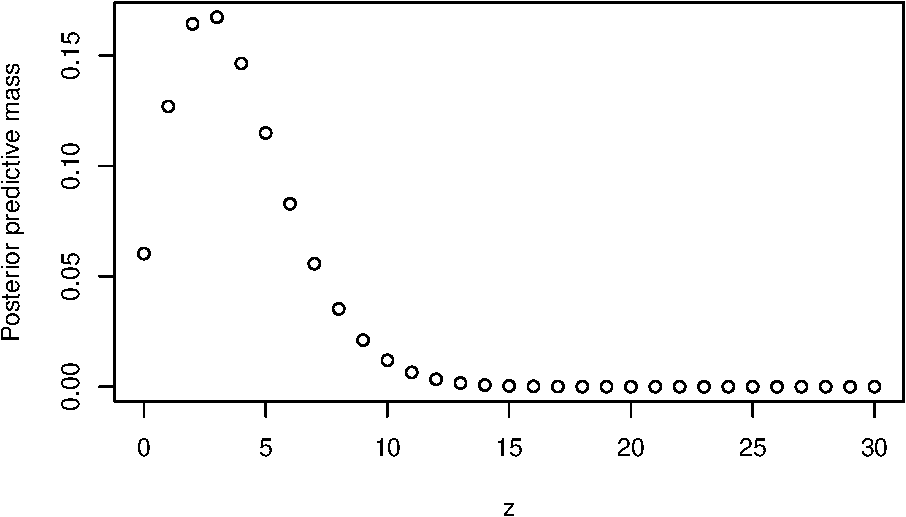
\includegraphics{_main_files/figure-latex/unnamed-chunk-14-1.pdf}

The expected number of students who hand in late is 3.75 and there's a 95\% chance that up to 8 hand in late.

\begin{Shaded}
\begin{Highlighting}[]
\NormalTok{z}\SpecialCharTok{\%*\%}\NormalTok{ppd }\CommentTok{\#expectation}
\end{Highlighting}
\end{Shaded}

\begin{verbatim}
##      [,1]
## [1,] 3.75
\end{verbatim}

\begin{Shaded}
\begin{Highlighting}[]
\FunctionTok{cbind}\NormalTok{(z, }\FunctionTok{cumsum}\NormalTok{(ppd)) }\CommentTok{\#CDF}
\end{Highlighting}
\end{Shaded}

\begin{verbatim}
##        z           
##  [1,]  0 0.06029453
##  [2,]  1 0.18723037
##  [3,]  2 0.35156696
##  [4,]  3 0.51889148
##  [5,]  4 0.66530044
##  [6,]  5 0.78021765
##  [7,]  6 0.86309065
##  [8,]  7 0.91880359
##  [9,]  8 0.95404202
## [10,]  9 0.97513714
## [11,] 10 0.98713498
## [12,] 11 0.99363285
## [13,] 12 0.99698773
## [14,] 13 0.99863936
## [15,] 14 0.99941423
## [16,] 15 0.99976022
## [17,] 16 0.99990696
## [18,] 17 0.99996591
## [19,] 18 0.99998826
## [20,] 19 0.99999622
## [21,] 20 0.99999887
## [22,] 21 0.99999969
## [23,] 22 0.99999992
## [24,] 23 0.99999998
## [25,] 24 1.00000000
## [26,] 25 1.00000000
## [27,] 26 1.00000000
## [28,] 27 1.00000000
## [29,] 28 1.00000000
## [30,] 29 1.00000000
## [31,] 30 1.00000000
\end{verbatim}

\end{example}

\hypertarget{non-informative-prior-distibrutions}{%
\section{Non-informative Prior Distibrutions}\label{non-informative-prior-distibrutions}}

We have seen in a few examples how the choice of the prior distribution (and prior parameters) can impact posterior distributions and the resulting conclusions. As the choice of prior distribution is subjective, it is the main criticism of Bayesian inference. A possible way around this is to use a prior distribution that reflects a lack of information about \(\theta\).

\begin{definition}
A \textbf{non-informative prior distribution} is a prior distribution that places equal weight on the every possible value of \(\theta\).
\end{definition}

\begin{example}
In Example \ref{exm:binom}, we assigned a uniform prior distribution to the parameter \(\theta\).
\end{example}

Such a prior distribution can have interesting and perhaps unintended side effects. Suppose we do indeed have some parameter \(\theta\) and we place a uniform prior distribution on \(\theta\) such that \(\theta \sim U[0, 1]\). This means, for example, our prior beliefs about \(\theta\) are that it is equally likely to be in \([0, 0.1]\) as it is to lie in \([0.8, 0.9]\) or any other interval of size 0.1. However, our prior beliefs about \(\theta^2\) are not uniform. Letting \(\psi = \theta^2\), changing variables gives \(\pi(\psi) = \frac{1}{2\sqrt{\psi}}\), something that is not uniform. That raises the question, if we have little to say about \(\theta\) \textit{a priori}, shouldn't we have little to say about any reasonable transformation of \(\theta\)?

\begin{theorem}[Jeffrey]
Given some observed data \(\boldsymbol{y} = \{y_1, \ldots, y_N\}\), an invariant prior distribution is
\[
\pi(\theta) \propto \sqrt{I_\theta(\boldsymbol{y})},
\]
where \(I_\theta(\boldsymbol{y})\) is the Fisher information for \(\theta\) contained in \(\boldsymbol{y}\).
\end{theorem}

Jeffrey argues that if there are two ways of parameterising a model, e.g.~via \(\theta\) and \(\psi\), then the priors on these parameters should be equivalent. In other words, the prior distribution should be invariant under sensible (one-to-one) transformations.

\begin{proof}
Recall that the distribution of \(\psi = h(\theta)\), for some one-to-one function \(h\), is invariant to the distribution of \(\theta\) if
\[
\pi(\psi) = \pi(\theta) \left|\frac{d\theta}{d\psi}\right|.
\]
Transforming the Fisher information for \(\psi\) shows
\begin{align*}
I_\psi({y}) &= - \mathbb{E}\left(\frac{d^2\log \pi({y} \mid \psi)}{d\psi^2}\right) \\
&= -\mathbb{E}\left(\frac{d}{d\psi} \left( \frac{d \log \pi(y|\theta(\psi))}{d \theta} \frac{d\theta}{d\psi} \right) \right) \tag{chain rule}\\
&= -\mathbb{E}\left(\left(\frac{d^2 \log \pi(y|\theta(\psi))}{d \theta d\psi}\right)\left( \frac{d\theta}{d\psi}\right) + \left(\frac{d \log \pi(y|\theta(\psi))}{d \theta}\right) \left( \frac{d^2\theta}{d\psi^2}\right) \right)\tag{prod. rule} \\
&= -\mathbb{E}\left(\left(\frac{d^2 \log \pi(y|\theta(\psi))}{d \theta^2 }\right)\left( \frac{d\theta}{d\psi}\right)^2 + \left(\frac{d \log \pi(y|\theta(\psi))}{d \theta}\right) \left( \frac{d^2\theta}{d\psi^2}\right) \right)\tag{chain rule} \\
& = -\mathbb{E}\left(\left(\frac{d^2 \log \pi({y} \mid \theta)}{d\theta^2}\left(\frac{d\theta}{d\psi}\right)^2\right)\right)  \\
& = I_\theta({y})\left(\frac{d\theta}{d\psi}\right)^2 .
\end{align*}
Thus \(\sqrt{I_\psi({y})} = \sqrt{I_\theta({y})} \left|\frac{d\theta}{d\psi}\right|\) and \(\sqrt{I_\psi({y})}\) and \(\sqrt{I_\theta({y})}\) are invariant prior distributions.
\end{proof}

\begin{example}
In Example \ref{exm:binom}, we modelled the number of bot accounts on a social media website by \(Y \sim \textrm{Bin}(n, \theta)\). To construct Jeffrey's prior distribution for \(\theta\), we must first derive the Fisher information.\\
\begin{align*}
&\pi(y \mid \theta) = \begin{pmatrix} n \\ y \end{pmatrix} \theta^y (1-\theta)^{n-y}\\ 
\implies &\log \pi(y \mid \theta) = \log \begin{pmatrix} n \\ y \end{pmatrix} + y \log\theta + (n-y)\log(1-\theta) \\
\implies &\frac{\partial \log \pi(y \mid \theta)}{\partial \theta} = \frac{y}{\theta} - \frac{n-y}{1-\theta} \\
\implies &\frac{\partial^2 \log \pi(y \mid \theta)}{\partial \theta^2} = -\frac{y}{\theta^2} + \frac{n-y}{(1-\theta)^2} \\
\implies &\mathbb{E}\left(\frac{\partial \log \pi(y \mid \theta)}{\partial \theta}\right) = -\frac{\mathbb{E}(y)}{\theta^2} + \frac{n-\mathbb{E}(y)}{(1-\theta)^2}\\ 
\implies &\mathbb{E}\left(\frac{\partial \log \pi(y \mid \theta)}{\partial \theta}\right) = -\frac{n\theta}{\theta^2} + \frac{n-n\theta}{(1-\theta)^2}\\ 
\implies &\mathbb{E}\left(\frac{\partial \log \pi(y \mid \theta)}{\partial \theta}\right) = -\frac{n}{\theta} + \frac{n}{1-\theta}\\
\implies &\mathbb{E}\left(\frac{\partial \log \pi(y \mid \theta)}{\partial \theta}\right) = -\frac{n}{\theta(1-\theta)} \\
\implies &I_\theta(y) \propto \frac{1}{\theta(1-\theta)}.
\end{align*}

Hence Jeffrey's prior is \(\pi(\theta) \propto \theta^{-\frac{1}{2}}(1-\theta)^{-\frac{1}{2}}\). This functional dependency on \(\theta\) shows that \(\theta \sim \textrm{Beta}(\frac{1}{2}, \frac{1}{2})\).
\end{example}

\hypertarget{bernstein-von-mises-theorem}{%
\section{Bernstein-von-Mises Theorem}\label{bernstein-von-mises-theorem}}

So far, we have considered Bayesian methods in contrast to frequentist ones. The Bernstein-von-Mises theorem is a key theorem linking the two inference methods.

\begin{theorem}[Bernstein-von-Mises]
For a well-specified model \(\pi(\boldsymbol{y} \mid \theta)\) with a fixed number of parameters, and for a smooth prior distribution \(\pi(\theta)\) that is non-zero around the MLE \(\hat{\theta}\), then
\[
\left|\left| \pi(\theta \mid \boldsymbol{y}) - N\left(\hat{\theta}, \frac{I(\hat{\theta})^{-1}}{n}\right) \right|\right|_{TV} \rightarrow 0,
\]
where \(||p - q||_{TV}\) is the total variation distance between distributions \(p\) and \(q\):
\[
||p - q||_{TV} = \frac{1}{2}\int|\pi(x) - q(x)|\,dx.
\]
\end{theorem}

The Berstein-von-Mises theorem says that as the number of data points approaches infinity, the posterior distribution tends to a Normal distribution centered around the MLE and variance dependent on the Fisher information. The proof of this theorem is out of the scope of this module, but can be found in Asymptotic Statistics (2000) by A. W. van der Vaart.

\hypertarget{lab}{%
\section{Lab}\label{lab}}

The aim of this lab is to work with some posterior distributions in cases when the prior distribution is or is not conjugate. Recall the definition of a conjugate prior distribution:

If the prior distribution \(\pi(\theta)\) has the same distributional family as the posterior distribution \(\pi(\theta \mid \boldsymbol{y})\), then the prior distribution is a \textbf{conjugate prior distribution}.

Working with conjugate prior distributions often makes the analytical work much easier, as we can work with the posterior distribution. But sometimes, conjugate prior distributions may not be appropriate. This is where R can help, as we do not need a closed form to carry out computations.

\begin{example}
The total number of goals scored in 50 games of a low level football league is shown below.

\begin{Shaded}
\begin{Highlighting}[]
\NormalTok{y }\OtherTok{\textless{}{-}} \FunctionTok{c}\NormalTok{(}\DecValTok{2}\NormalTok{, }\DecValTok{6}\NormalTok{, }\DecValTok{2}\NormalTok{, }\DecValTok{3}\NormalTok{, }\DecValTok{4}\NormalTok{, }\DecValTok{3}\NormalTok{, }\DecValTok{4}\NormalTok{, }\DecValTok{3}\NormalTok{, }\DecValTok{1}\NormalTok{, }\DecValTok{2}\NormalTok{, }\DecValTok{3}\NormalTok{, }\DecValTok{2}\NormalTok{, }\DecValTok{6}\NormalTok{, }\DecValTok{6}\NormalTok{, }\DecValTok{2}\NormalTok{, }\DecValTok{3}\NormalTok{, }\DecValTok{5}\NormalTok{, }\DecValTok{1}\NormalTok{, }\DecValTok{2}\NormalTok{, }\DecValTok{2}\NormalTok{, }\DecValTok{4}\NormalTok{, }\DecValTok{2}\NormalTok{, }\DecValTok{5}\NormalTok{, }\DecValTok{3}\NormalTok{,}
       \DecValTok{6}\NormalTok{, }\DecValTok{4}\NormalTok{, }\DecValTok{1}\NormalTok{, }\DecValTok{2}\NormalTok{, }\DecValTok{7}\NormalTok{, }\DecValTok{8}\NormalTok{, }\DecValTok{4}\NormalTok{, }\DecValTok{3}\NormalTok{, }\DecValTok{7}\NormalTok{, }\DecValTok{3}\NormalTok{, }\DecValTok{3}\NormalTok{, }\DecValTok{5}\NormalTok{, }\DecValTok{2}\NormalTok{, }\DecValTok{6}\NormalTok{, }\DecValTok{1}\NormalTok{, }\DecValTok{3}\NormalTok{, }\DecValTok{7}\NormalTok{, }\DecValTok{4}\NormalTok{, }\DecValTok{2}\NormalTok{, }\DecValTok{6}\NormalTok{, }\DecValTok{8}\NormalTok{, }\DecValTok{8}\NormalTok{, }\DecValTok{4}\NormalTok{, }\DecValTok{5}\NormalTok{,}
       \DecValTok{7}\NormalTok{, }\DecValTok{4}\NormalTok{)}
\FunctionTok{hist}\NormalTok{(y, }\AttributeTok{main =} \StringTok{""}\NormalTok{, }\AttributeTok{xlab =} \StringTok{"Number of goals scored"}\NormalTok{)}
\end{Highlighting}
\end{Shaded}

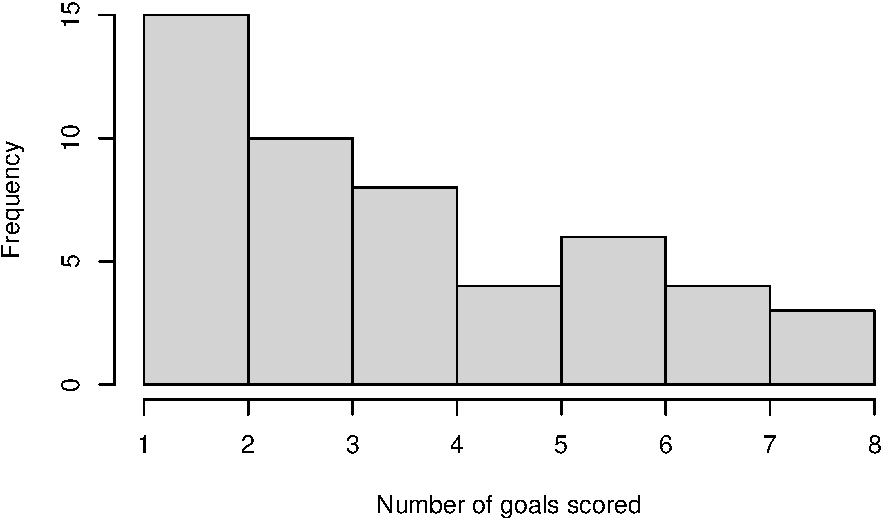
\includegraphics{_main_files/figure-latex/unnamed-chunk-16-1.pdf}

\begin{Shaded}
\begin{Highlighting}[]
\FunctionTok{mean}\NormalTok{(y)}
\end{Highlighting}
\end{Shaded}

\begin{verbatim}
## [1] 3.92
\end{verbatim}

We can model the number of goals scored using a Poisson distribution
\[
y \sim \hbox{Po}(\lambda).
\]
By Bayes' theorem, the posterior distribution is given by
\[
\pi(\lambda \mid \boldsymbol{y}) \propto \pi(\boldsymbol{y} \mid \lambda)\pi(\lambda). 
\]
The likelihood function is given by
\begin{align*}
\pi(\boldsymbol{y} \mid \lambda) &= \prod_{i=1}^{50} \frac{e^{-\lambda}\lambda^{y_i}}{y_i!}\\
&= \frac{e^{-50\lambda}\lambda^{\sum y_i}}{\prod_{i=1}^{50} y_i!} 
\end{align*}

R has a set of inbuilt functions for working with the Poisson distribution so we can rely on those to write functions for the likelihood and loglikelihood.

\begin{Shaded}
\begin{Highlighting}[]
\NormalTok{lambda }\OtherTok{\textless{}{-}} \FunctionTok{seq}\NormalTok{(}\DecValTok{0}\NormalTok{, }\DecValTok{10}\NormalTok{, }\FloatTok{0.01}\NormalTok{) }\CommentTok{\#grid of lambda values}
\NormalTok{likelihood.function }\OtherTok{\textless{}{-}} \ControlFlowTok{function}\NormalTok{(lambda, y) }\FunctionTok{prod}\NormalTok{(}\FunctionTok{dpois}\NormalTok{(y, lambda)) }\CommentTok{\#compute likelihood}
\NormalTok{log.likelihood.function  }\OtherTok{\textless{}{-}} \ControlFlowTok{function}\NormalTok{(lambda, y) }\FunctionTok{sum}\NormalTok{(}\FunctionTok{dpois}\NormalTok{(y, lambda, }\AttributeTok{log =} \ConstantTok{TRUE}\NormalTok{)) }\CommentTok{\#compute loglikelihood}
\NormalTok{likelihood }\OtherTok{\textless{}{-}} \FunctionTok{sapply}\NormalTok{(lambda,  likelihood.function, y) }\CommentTok{\#evaluate at grid of points}
\NormalTok{log.likelihood }\OtherTok{\textless{}{-}} \FunctionTok{sapply}\NormalTok{(lambda,  log.likelihood.function, y) }\CommentTok{\#evaluate at grid of points}

\CommentTok{\#Plot likelihood}
\FunctionTok{plot}\NormalTok{(lambda, likelihood, }
     \AttributeTok{xlab =} \FunctionTok{expression}\NormalTok{(lambda), }\AttributeTok{ylab =} \StringTok{"likelihood"}\NormalTok{, }\AttributeTok{type =} \StringTok{\textquotesingle{}l\textquotesingle{}}\NormalTok{)}
\end{Highlighting}
\end{Shaded}

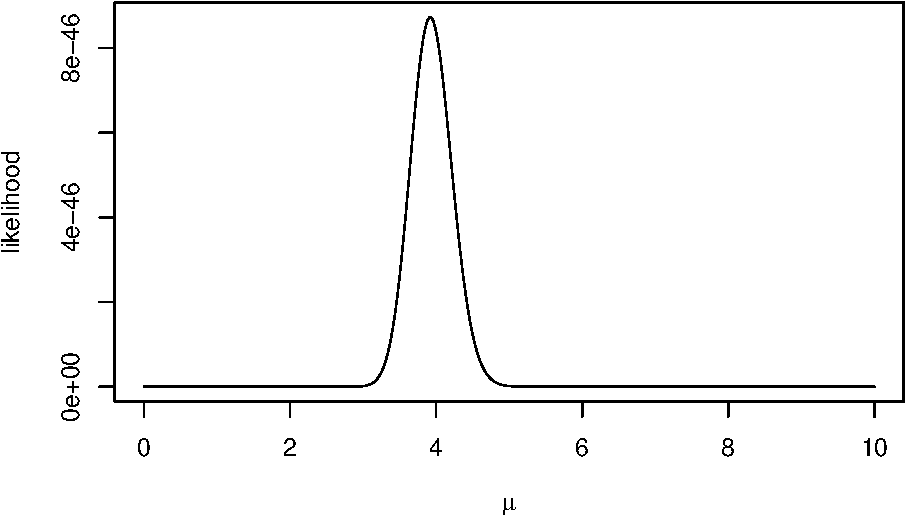
\includegraphics{_main_files/figure-latex/unnamed-chunk-17-1.pdf}

\begin{Shaded}
\begin{Highlighting}[]
\FunctionTok{plot}\NormalTok{(lambda, log.likelihood, }
     \AttributeTok{xlab =} \FunctionTok{expression}\NormalTok{(lambda), }\AttributeTok{ylab =} \StringTok{"loglikelihood"}\NormalTok{, }\AttributeTok{type =} \StringTok{\textquotesingle{}l\textquotesingle{}}\NormalTok{)}
\end{Highlighting}
\end{Shaded}

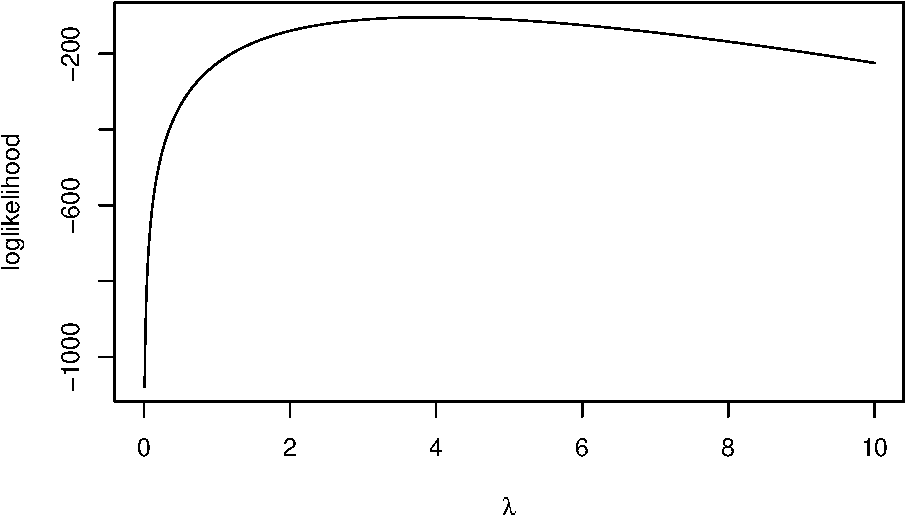
\includegraphics{_main_files/figure-latex/unnamed-chunk-17-2.pdf}
When coding posterior distributions, we often work on the log scale because the numbers can be smaller that R can deal with. The denominator with the factorial can get very large very quickly.

After speaking to football experts, we decide to place a normal prior distribution on \(\lambda\) with mean 5 goals and standard deviation one goal, i.e.
\[
\lambda \sim N(5, 1).
\]
The prior distribution can be plotted by

\begin{Shaded}
\begin{Highlighting}[]
\NormalTok{lambda   }\OtherTok{\textless{}{-}} \FunctionTok{seq}\NormalTok{(}\DecValTok{0}\NormalTok{, }\DecValTok{10}\NormalTok{, }\FloatTok{0.01}\NormalTok{) }\CommentTok{\#grid of lambda values}
\NormalTok{prior    }\OtherTok{\textless{}{-}} \FunctionTok{dnorm}\NormalTok{(lambda, }\DecValTok{5}\NormalTok{, }\DecValTok{1}\NormalTok{)}
\NormalTok{log.prior }\OtherTok{\textless{}{-}} \FunctionTok{dnorm}\NormalTok{(lambda, }\DecValTok{5}\NormalTok{, }\DecValTok{1}\NormalTok{, }\AttributeTok{log =} \ConstantTok{TRUE}\NormalTok{)}
\FunctionTok{plot}\NormalTok{(lambda, prior, }\AttributeTok{type =} \StringTok{\textquotesingle{}l\textquotesingle{}}\NormalTok{, }\AttributeTok{xlab =} \FunctionTok{expression}\NormalTok{(lambda), }\AttributeTok{ylab =} \StringTok{"density"}\NormalTok{)}
\end{Highlighting}
\end{Shaded}

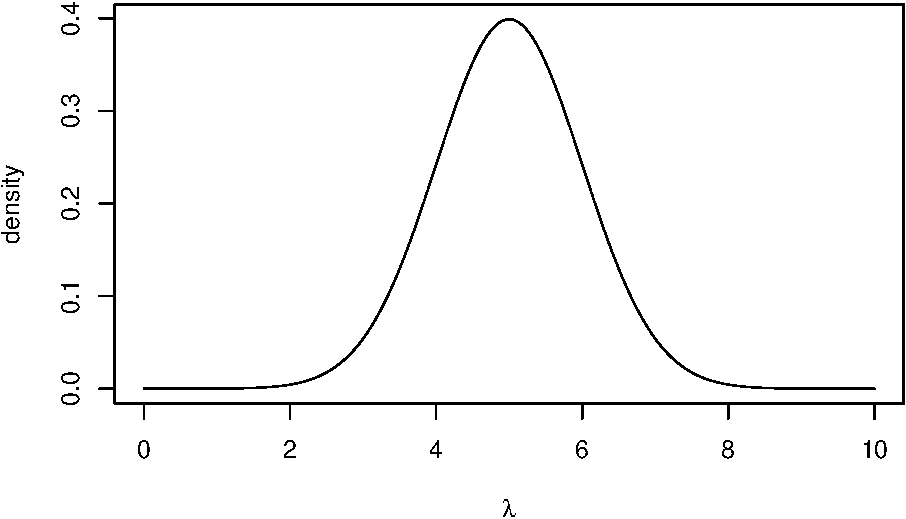
\includegraphics{_main_files/figure-latex/unnamed-chunk-18-1.pdf}

\begin{Shaded}
\begin{Highlighting}[]
\FunctionTok{plot}\NormalTok{(lambda, log.prior, }\AttributeTok{type =} \StringTok{\textquotesingle{}l\textquotesingle{}}\NormalTok{, }
     \AttributeTok{xlab =} \FunctionTok{expression}\NormalTok{(lambda), }\AttributeTok{ylab =} \StringTok{"log density"}\NormalTok{)}
\end{Highlighting}
\end{Shaded}

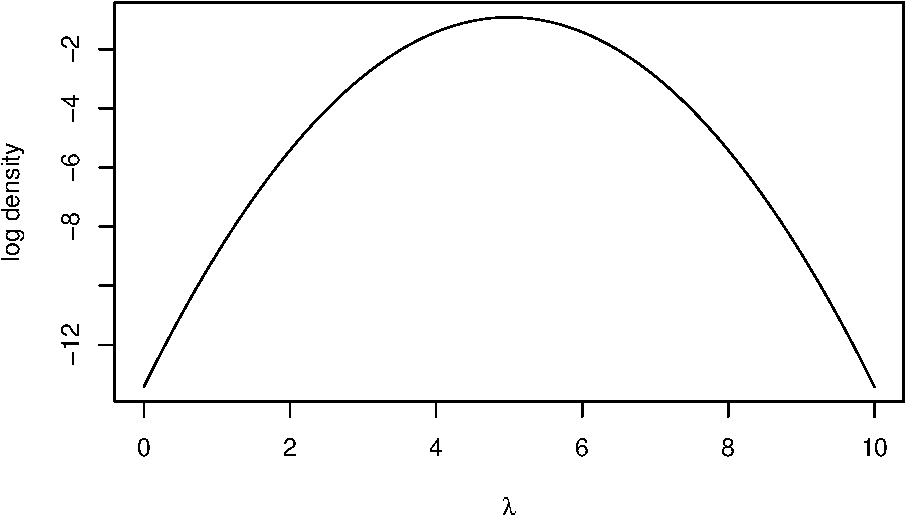
\includegraphics{_main_files/figure-latex/unnamed-chunk-18-2.pdf}

Writing the posterior distribution up to proportionality, we get
\[
\pi(\lambda \mid \boldsymbol{y}) \propto \exp\left(-50\lambda -\frac{1}{2}(\lambda - 5)^2\right)\lambda^{\sum y_i}.
\]
There is no closed form for this distribution and it is not that nice to work with. But with R, we can easily evaluate the posterior distribution at a grid of points.

\begin{Shaded}
\begin{Highlighting}[]
\NormalTok{posterior }\OtherTok{\textless{}{-}}\NormalTok{ prior}\SpecialCharTok{*}\NormalTok{likelihood}
\NormalTok{integrating.factor }\OtherTok{\textless{}{-}} \FloatTok{0.5}\SpecialCharTok{*}\FloatTok{0.01}\SpecialCharTok{*}\NormalTok{(posterior[}\DecValTok{1}\NormalTok{] }\SpecialCharTok{+}\NormalTok{ posterior[}\DecValTok{1001}\NormalTok{] }\SpecialCharTok{+} \DecValTok{2}\SpecialCharTok{*}\FunctionTok{sum}\NormalTok{(posterior[}\SpecialCharTok{{-}}\FunctionTok{c}\NormalTok{(}\DecValTok{1}\NormalTok{, }\DecValTok{1001}\NormalTok{)])) }\CommentTok{\#Using trapezium rule}
\NormalTok{posterior }\OtherTok{\textless{}{-}}\NormalTok{ posterior}\SpecialCharTok{/}\NormalTok{integrating.factor }\CommentTok{\#normalise}
\FunctionTok{plot}\NormalTok{(lambda, posterior, }\AttributeTok{type =} \StringTok{\textquotesingle{}l\textquotesingle{}}\NormalTok{, }\AttributeTok{xlab =} \FunctionTok{expression}\NormalTok{(lambda), }
     \AttributeTok{ylab =} \StringTok{"posterior density"}\NormalTok{)}
\end{Highlighting}
\end{Shaded}

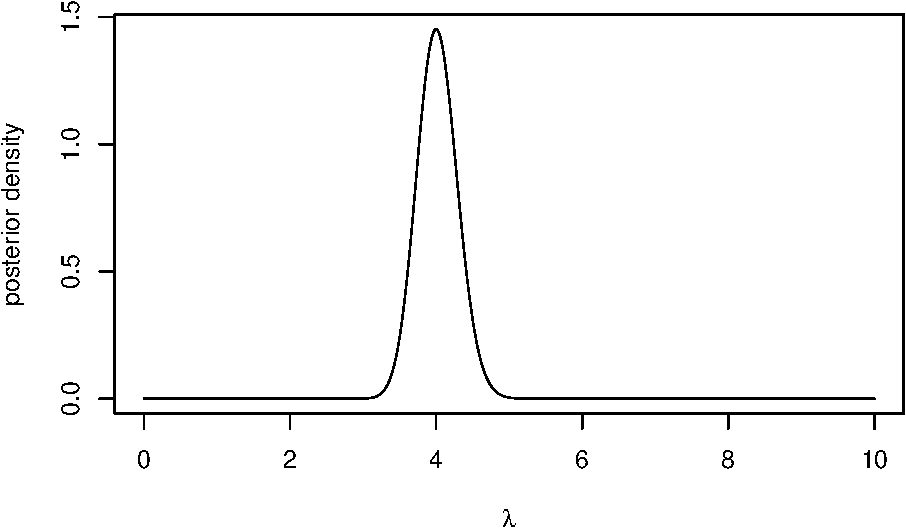
\includegraphics{_main_files/figure-latex/unnamed-chunk-19-1.pdf}

We can now visually inspect the posterior distribution and see that it has a strong peak around 4. One important statistic is the \textbf{maximum a posteriori estimation} or MAP estimate, this is the mode of the posterior distribution and it is a similar principle to the maximum likelihood estimate.

We can compute this using the command

\begin{Shaded}
\begin{Highlighting}[]
\NormalTok{lambda[}\FunctionTok{which.max}\NormalTok{(posterior)]}
\end{Highlighting}
\end{Shaded}

\begin{verbatim}
## [1] 4
\end{verbatim}

which shows the MAP estimate is exactly 4.
\end{example}

\begin{exercise}
Adapt the code in the Example above to use an exponential prior distribution with rate 0.1. Then derive the posterior distribution analytically and compare to the numerical version.
\end{exercise}

\begin{exercise}

You are given that the data are exponentially distributed with rate \(\lambda,\) i.e.~\(Y_1, \ldots, Y_N \sim \hbox{Exp}(\lambda)\). Your prior belief is that \(\lambda \in (0, 1)\). Show that the posterior distribution \(\pi(\lambda \mid \boldsymbol{y})\) has no closed form when the prior distribution for \(\lambda \sim \hbox{Beta}(\alpha, \beta)\).

The data is given by

\begin{Shaded}
\begin{Highlighting}[]
\NormalTok{y }\OtherTok{\textless{}{-}} \FunctionTok{c}\NormalTok{(}\FloatTok{1.101558}\NormalTok{, }\FloatTok{1.143953}\NormalTok{, }\FloatTok{1.287348}\NormalTok{, }\FloatTok{1.181010}\NormalTok{, }\FloatTok{1.139132}\NormalTok{, }\FloatTok{1.148631}\NormalTok{, }\FloatTok{1.133201}\NormalTok{, }\FloatTok{1.361229}\NormalTok{, }\FloatTok{1.332540}\NormalTok{, }\FloatTok{1.052501}\NormalTok{)}
\end{Highlighting}
\end{Shaded}

\end{exercise}

By writing an R function to evaluate the likelihood function, evaluate the posterior distribution for \(\lambda\) over a grid of points.

\begin{exercise}

Suppose you have \(X_1, ..., X_N \sim \hbox{Bin}(100, p)\). Using \(p \sim \hbox{Beta}(\alpha, \beta)\) as the prior distribution, derive the posterior distribution and the posterior mean (Wikipedia is a helpful place for properties of distributions).

\begin{enumerate}
\def\labelenumi{\arabic{enumi}.}
\tightlist
\item
  (Large data scenario) Fix \(\alpha = 2\), \(N = 150\) and \(\Sigma x_i = 2,971\). Plot the prior and posterior distributions for different values of \(\beta\) on the same figure. Plot the posterior mean against \(\beta \in (0, 10)\). Plot the prior mean against the posterior mean for \(\beta \in (0, 10)\).
\item
  (Small data scenario) Fix \(\alpha = 2\), \(N = 10\) and \(\Sigma x_i = 101\) Plot the prior and posterior distributions for different values of \(\beta\) on the same figure.Plot the posterior distribution for different values of \(\beta\). Plot the posterior mean against \(\beta \in (0, 10)\). Plot the prior mean against the posterior mean for \(\beta \in (0, 10)\).
\end{enumerate}

\end{exercise}

\begin{exercise}
Code up the posterior distribution in question 4 of problem sheet 2 (the Pareto distribution). Set \(a = 1\), \(b = 2\) and let the data be

\begin{verbatim}
y <- c(1.019844, 1.043574, 1.360953, 1.049228, 1.491926, 1.192943, 1.323738, 1.262572, 2.034768, 1.451654)
\end{verbatim}

Find the MAP estimate for \(\beta\)
\end{exercise}

\hypertarget{sampling}{%
\chapter{Sampling}\label{sampling}}

\hypertarget{uniform-random-numbers}{%
\section{Uniform Random Numbers}\label{uniform-random-numbers}}

What we won't be doing in this module is generating true uniform random numbers. This is incredibly difficult and usually requires lots of expensive hardware. This is because computers aren't good at being random, they require algorithmic instructions. True random number generation often uses physical methods, such as the radioactive decay of atoms, or atmospheric noise.

Throughout this module, we will be using R's built in random number generation. This is a pseudo random number generator that has excellent random properties, but will eventually repeat. A basic random number generation tool that we will repeatedly use in the module involves sampling from a uniform distribution on the unit interval, which can be done in R using

\begin{Shaded}
\begin{Highlighting}[]
\FunctionTok{runif}\NormalTok{(}\DecValTok{1}\NormalTok{, }\DecValTok{0}\NormalTok{, }\DecValTok{1}\NormalTok{)}
\end{Highlighting}
\end{Shaded}

\begin{verbatim}
## [1] 0.1374065
\end{verbatim}

\hypertarget{inverse-transform-sampling}{%
\section{Inverse Transform Sampling}\label{inverse-transform-sampling}}

Suppose we want to sample from a non-uniform one-dimensional distribution. The inverse transform theorem allows us to do this using the distribution's inverse function.

\begin{definition}
Let \(X\) be a real-valued random variable with a distribution function \(F\). Then the \textbf{inverse function} of a distribution function \(F\), denoted \(F^{-1}\), is defined for all \(u \in (0, 1)\) by
\[
F^{-1}(u) = \inf\{x \in\mathbb{R} : F(x) > u\}.
\]
\end{definition}

\begin{theorem}
Let \(F :\mathbb{R} \rightarrow [0, 1]\) be a continuous distribution function, \(U \sim U[0, 1]\) and \(Y = F^{-1}(U)\). Then \(Y\) has distribution function \(F\).
\end{theorem}

\begin{proof}
We have
\[
\mathbb{P}(Y \leq a) = \mathbb{P}(F^{-1}(U) \leq a) = \mathbb{P}(\inf\{x \in\mathbb{R} : F(x) > u\} \leq a). 
\]
Since \(\inf\{x \in\mathbb{R} : F(x) > u\} \leq a\) can only hold if \(F(a) \geq U\), we have
\[
\mathbb{P}(Y \leq a)  = \mathbb{P}(F(a)\geq U)
\]
As \(U \sim U[0, 1]\), we have \(\mathbb{P}(F(a)\geq U) = F(a)\).
\end{proof}

This theorem says that if we have a random variable \(U \sim U[0, 1]\) and we want to get \(Y \sim F\), then we can use \(F^{-1}(U)\). Viewing this theorem graphically can provide a much more intuitive understanding.

\begin{example}
We would like to sample from an exponential distribution with rate \(\lambda\), i.e.~\(Y ~ \sim \hbox{Exp}(\lambda)\). The density function is given by

\[
\pi(y \mid \lambda) = \begin{cases} 
      \lambda e^{\lambda y} & y \geq 0 \\
    0  & \text{otherwise.}
   \end{cases}
\]

The distribution function can be derived by
\begin{align*}
F(y \mid \lambda) &= \int_0^y \lambda e^{\lambda t}\,dt \\
& =  1 - e^{\lambda y}.
\end{align*}
Finally, the inverse function is given by
\[
F^{-1}(y \mid \lambda) = -\frac{1}{\lambda}\log(1-y).  
\]
Therefore, if \(U \sim U[0, 1]\), then it follows that \(-\frac{1}{\lambda}log(1-U) \sim \hbox{Exp}(\lambda)\).

The R code below generates a plot to show this (with \(\lambda = 0.5\)). We can plot the CDF for most one parameter distributions straightforwardly. We can think of this theorem as allowing us to sample a point on the y-axis and then computing the quantile this corresponds to.

\begin{Shaded}
\begin{Highlighting}[]
\FunctionTok{set.seed}\NormalTok{(}\DecValTok{12345}\NormalTok{) }\CommentTok{\# to reproduce}
\NormalTok{y }\OtherTok{\textless{}{-}} \FunctionTok{seq}\NormalTok{(}\DecValTok{0}\NormalTok{, }\DecValTok{10}\NormalTok{, }\FloatTok{0.01}\NormalTok{) }\CommentTok{\#Show on the interval [0, 5]}
\NormalTok{f }\OtherTok{\textless{}{-}} \DecValTok{1} \SpecialCharTok{{-}} \FunctionTok{exp}\NormalTok{(}\SpecialCharTok{{-}}\FloatTok{0.5}\SpecialCharTok{*}\NormalTok{y)    }\CommentTok{\#Construct the cumulative density }
                        \CommentTok{\#function (CDF)}
\FunctionTok{plot}\NormalTok{(y, f, }\AttributeTok{type =}\StringTok{\textquotesingle{}l\textquotesingle{}}\NormalTok{, }\AttributeTok{xlab =} \StringTok{"y"}\NormalTok{, }\AttributeTok{ylab=} \StringTok{"CDF"}\NormalTok{)}

\CommentTok{\#Sample u}
\NormalTok{u }\OtherTok{\textless{}{-}} \FunctionTok{runif}\NormalTok{(}\DecValTok{1}\NormalTok{)}

\CommentTok{\#Get the corresponding y value}
\NormalTok{f.inv }\OtherTok{\textless{}{-}} \SpecialCharTok{{-}}\DecValTok{2}\SpecialCharTok{*}\FunctionTok{log}\NormalTok{(}\DecValTok{1}\SpecialCharTok{{-}}\NormalTok{u)}

\CommentTok{\#plot }
\FunctionTok{segments}\NormalTok{(}\AttributeTok{x0 =} \DecValTok{0}\NormalTok{, }\AttributeTok{y0 =}\NormalTok{ u, }\AttributeTok{x1 =}\NormalTok{ f.inv, }\AttributeTok{y1 =}\NormalTok{ u, }\AttributeTok{lty =} \DecValTok{2}\NormalTok{)}
\FunctionTok{segments}\NormalTok{(}\AttributeTok{x0 =}\NormalTok{ f.inv, }\AttributeTok{y0 =} \DecValTok{0}\NormalTok{, }\AttributeTok{x1 =}\NormalTok{ f.inv, }\AttributeTok{y1 =}\NormalTok{ u, }\AttributeTok{lty =} \DecValTok{2}\NormalTok{)}
\FunctionTok{text}\NormalTok{(}\AttributeTok{x =}\NormalTok{ f.inv, }\AttributeTok{y =} \SpecialCharTok{{-}}\FloatTok{0.01}\NormalTok{, }\FunctionTok{expression}\NormalTok{(F[}\SpecialCharTok{{-}}\DecValTok{1}\NormalTok{](U)), }\AttributeTok{col =} \DecValTok{4}\NormalTok{)}
\FunctionTok{text}\NormalTok{(}\AttributeTok{x =} \SpecialCharTok{{-}}\NormalTok{.}\DecValTok{1}\NormalTok{, }\AttributeTok{y =}\NormalTok{ u, }\StringTok{"U"}\NormalTok{, }\AttributeTok{col =} \DecValTok{4}\NormalTok{)}
\end{Highlighting}
\end{Shaded}

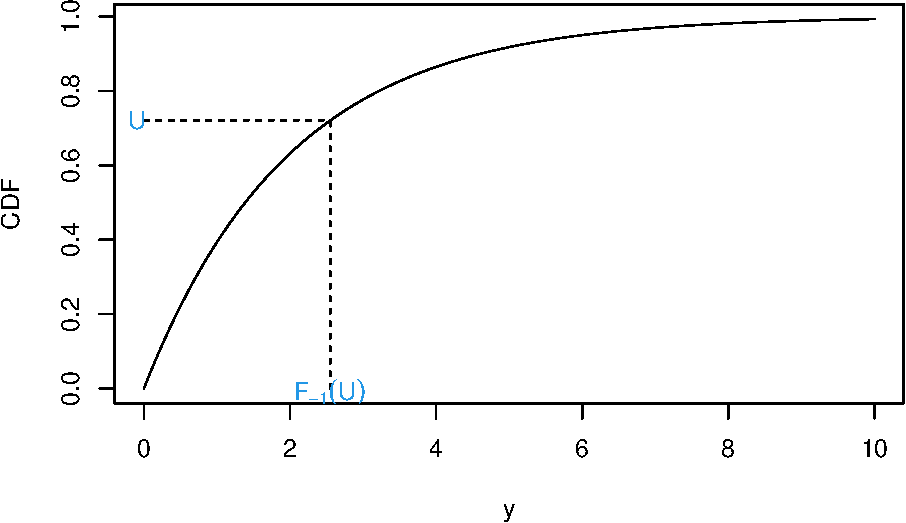
\includegraphics{_main_files/figure-latex/unnamed-chunk-23-1.pdf}
\end{example}

\begin{example}
Suppose we want to generate samples from the Cauchy distribution with location 0 and scale 1. This has density function
\[
\pi(x) = \frac{1}{\pi(1+x^2)}, \quad x \in \mathbb{R}.
\]
A plot of this function is shown below.

\begin{Shaded}
\begin{Highlighting}[]
\NormalTok{x }\OtherTok{\textless{}{-}} \FunctionTok{seq}\NormalTok{(}\SpecialCharTok{{-}}\DecValTok{5}\NormalTok{, }\DecValTok{5}\NormalTok{, }\FloatTok{0.01}\NormalTok{)}
\NormalTok{y }\OtherTok{\textless{}{-}} \DecValTok{1}\SpecialCharTok{/}\NormalTok{(pi}\SpecialCharTok{*}\NormalTok{(}\DecValTok{1} \SpecialCharTok{+}\NormalTok{ x}\SpecialCharTok{\^{}}\DecValTok{2}\NormalTok{))}
\FunctionTok{plot}\NormalTok{(x, y, }\AttributeTok{type =} \StringTok{\textquotesingle{}l\textquotesingle{}}\NormalTok{)}
\end{Highlighting}
\end{Shaded}

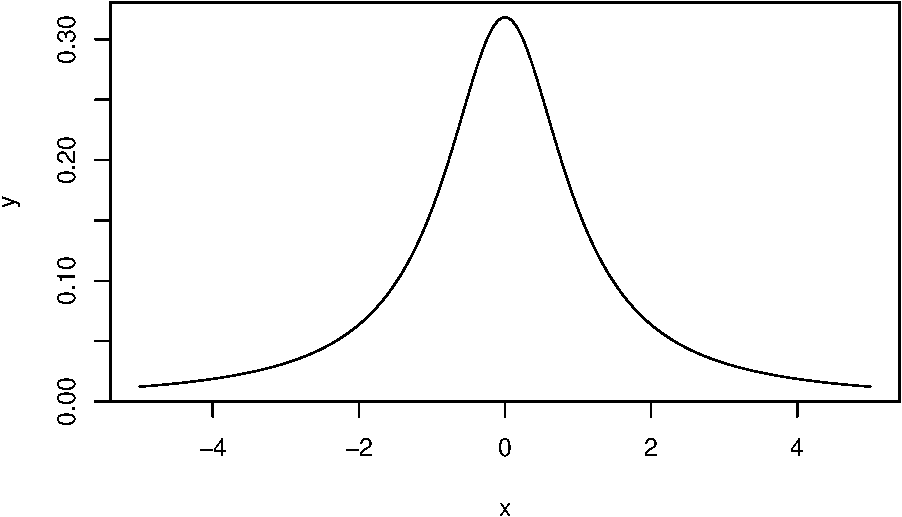
\includegraphics{_main_files/figure-latex/unnamed-chunk-24-1.pdf}
To use the inverse transform method, we first need to find the CDF:
\[
F(x) = \int_{-\infty}^x \frac{1}{\pi(1+t^2)}dt
\]
Letting \(t = \tan \theta\), we can write \(dt = \sec^2(\theta)d\theta\). The integral becomes
\[
F(x) = \int_{-\frac{\pi}{2}}^{\arctan(x)} \frac{\sec^2(\theta)}{\pi(1+\tan^2(\theta))} d\theta
\]
As \(1 + \tan^2(\theta) = \sec^2(\theta)\), we can write the integral as
\[
F(x) = \int_{-\frac{\pi}{2}}^{\arctan(x)} \frac{1}{\pi}du\\
= \left[\frac{\theta}{\pi}\right]_{-\frac{\pi}{2}}^{\arctan(x)}\\
= \frac{\arctan(x)}{\pi} + \frac{1}{2}.
\]
The inverse of the distribution function is
\[
F^{-1}(x) = \tan\left(\pi\left(x - \frac{1}{2}\right)\right).
\]
Hence, if \(U \sim U[0, 1]\), then \(\tan\left(\pi\left(U - \frac{1}{2}\right)\right) \sim \hbox{Cauchy}(0, 1)\).
\end{example}

\hypertarget{rejection-sampling}{%
\section{Rejection Sampling}\label{rejection-sampling}}

We now have a way of sampling realisations from distributions where we can analytically derive the inverse distribution function. We can use this to sample from more complex densities, or simple densities more efficiently. Rejection sampling works by sampling according to a density we can sample from and then rejecting or accepting that sample based on the density we're actually interested in. The plot below shows an example from this. We would like to generate a sample from the distribution with the curved density function, which is challenging. Instead, we find a distribution whose density function bounds the one we are interested in a sample from that. In this case we can use the uniform distribution. Once we have generated our sample from he uniform distribution, we choose to accept or reject it based on the distribution we are interested in. In this case we reject it.

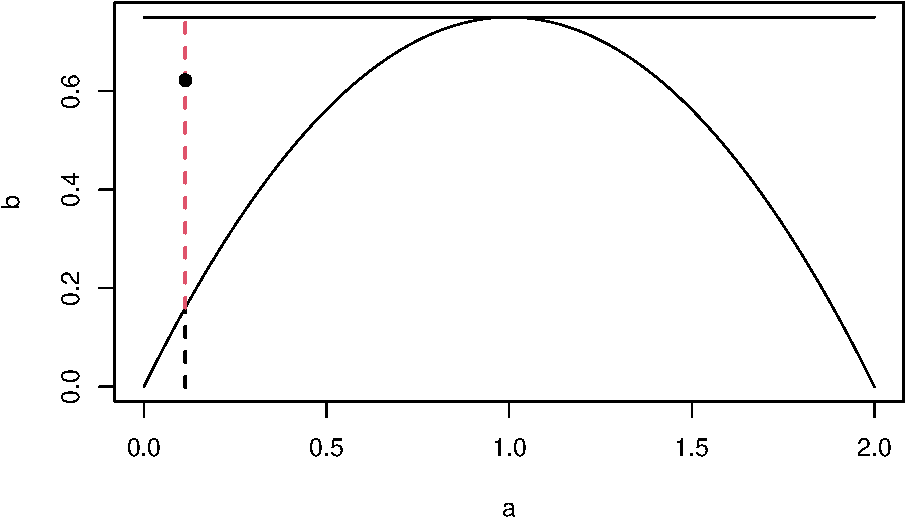
\includegraphics{_main_files/figure-latex/unnamed-chunk-25-1.pdf}

Suppose we want to sample from a density \(\pi\), but can only generate samples from a density \(q\). If there exists some constant \(c > 0\), such that \(\frac{\pi(y)}{q(y)} \leq c\) for all \(y\), then we can generate samples from \(\pi\) by

\begin{enumerate}
\def\labelenumi{\arabic{enumi}.}
\item
  Sampling \(Y \sim Q\)
\item
  Sampling \(U \sim U[0, 1]\)
\item
  Computing \(k = \frac{\pi(u)}{cq(y)}\)
\item
  Accepting \(y\) if \(U < k\) and rejecting otherwise.
\end{enumerate}

This says draw sample a point \(y\) according to the density \(q\). Draw a vertical line at \(y\) from the \(x\)-axis to \(cq(y)\). Sample uniformly on this line. If the uniformly random sample is below \(q\), then accept it. Otherwise, reject it. The theory behind this is as follows. Suppose we sample some point y according to this algorithm and we want to work out its density \(f\), then
\[
f(y) \propto q(y)\pi(U < k) = q(y)\frac{\pi(u)}{cq(y)} = \frac{\pi(u)}{c}.
\]
Therefore, \(f = p\).

\begin{example}
Suppose we want to sample from a distribution that has the density
\[
\pi(y) = \begin{cases}
\frac{3}{4}y(2-y), \qquad y \in [0, 2] \\
0, \qquad \textrm{otherwise}
\end{cases}.
\]
This has a maximum at \(\frac{3}{4}\). We choose \(p \sim U[0, 1]\) and \(c = \frac{3}{2}\). The R code below shows a pictorial version of how one sample is generated.

\begin{Shaded}
\begin{Highlighting}[]
\FunctionTok{set.seed}\NormalTok{(}\DecValTok{1234}\NormalTok{)   }\CommentTok{\#to reproduce}
\NormalTok{scaling.c }\OtherTok{\textless{}{-}} \DecValTok{3}\SpecialCharTok{/}\DecValTok{2}         \CommentTok{\#set c}
\NormalTok{y }\OtherTok{\textless{}{-}} \FunctionTok{runif}\NormalTok{(}\DecValTok{1}\NormalTok{, }\DecValTok{0}\NormalTok{, }\DecValTok{2}\NormalTok{)    }\CommentTok{\#sample Y \textasciitilde{} Q}
\NormalTok{p }\OtherTok{\textless{}{-}} \DecValTok{3}\SpecialCharTok{/}\DecValTok{4}\SpecialCharTok{*}\NormalTok{y}\SpecialCharTok{*}\NormalTok{(}\DecValTok{2}\SpecialCharTok{{-}}\NormalTok{y) }\CommentTok{\#compute pi(y)}
\NormalTok{k }\OtherTok{\textless{}{-}}\NormalTok{ p}\SpecialCharTok{/}\NormalTok{(scaling.c}\SpecialCharTok{*}\DecValTok{1}\SpecialCharTok{/}\DecValTok{2}\NormalTok{)     }\CommentTok{\#compute k}
\NormalTok{u }\OtherTok{\textless{}{-}} \FunctionTok{runif}\NormalTok{(}\DecValTok{1}\NormalTok{)    }\CommentTok{\#sample U \textasciitilde{} U[0, 1]}
\FunctionTok{ifelse}\NormalTok{(u }\SpecialCharTok{\textless{}}\NormalTok{ k, }\StringTok{\textquotesingle{}accept\textquotesingle{}}\NormalTok{, }\StringTok{\textquotesingle{}reject\textquotesingle{}}\NormalTok{) }\CommentTok{\#Accept if  u \textless{} k}
\end{Highlighting}
\end{Shaded}

\begin{verbatim}
## [1] "reject"
\end{verbatim}

\begin{Shaded}
\begin{Highlighting}[]
\CommentTok{\#Create nice plot}
\NormalTok{a }\OtherTok{\textless{}{-}} \FunctionTok{seq}\NormalTok{(}\DecValTok{0}\NormalTok{, }\DecValTok{2}\NormalTok{, }\FloatTok{0.01}\NormalTok{)}
\NormalTok{b }\OtherTok{\textless{}{-}} \DecValTok{3}\SpecialCharTok{/}\DecValTok{4}\SpecialCharTok{*}\NormalTok{a}\SpecialCharTok{*}\NormalTok{(}\DecValTok{2}\SpecialCharTok{{-}}\NormalTok{a)}
\NormalTok{scaling.c  }\OtherTok{\textless{}{-}}\NormalTok{ scaling.c}\SpecialCharTok{*}\FunctionTok{rep}\NormalTok{(}\DecValTok{1}\NormalTok{, }\FunctionTok{length}\NormalTok{(a))}
\FunctionTok{plot}\NormalTok{(a, b, }\AttributeTok{ylim =} \FunctionTok{c}\NormalTok{(}\DecValTok{0}\NormalTok{, }\DecValTok{3}\SpecialCharTok{/}\DecValTok{2}\NormalTok{), }\AttributeTok{type =} \StringTok{\textquotesingle{}l\textquotesingle{}}\NormalTok{)}
\FunctionTok{lines}\NormalTok{(a, scaling.c)}
\FunctionTok{segments}\NormalTok{(}\AttributeTok{x0 =}\NormalTok{ y, }\AttributeTok{y0 =} \DecValTok{0}\NormalTok{, }\AttributeTok{x1 =}\NormalTok{ y,  }\AttributeTok{y1 =}\DecValTok{3}\SpecialCharTok{/}\DecValTok{4}\SpecialCharTok{*}\NormalTok{y}\SpecialCharTok{*}\NormalTok{(}\DecValTok{2}\SpecialCharTok{{-}}\NormalTok{y) , }
          \AttributeTok{lty =} \DecValTok{2}\NormalTok{, }\AttributeTok{lwd =} \DecValTok{2}\NormalTok{)}
\FunctionTok{segments}\NormalTok{(}\AttributeTok{x0 =}\NormalTok{ y,  }\AttributeTok{y0 =}\DecValTok{3}\SpecialCharTok{/}\DecValTok{4}\SpecialCharTok{*}\NormalTok{y}\SpecialCharTok{*}\NormalTok{(}\DecValTok{2}\SpecialCharTok{{-}}\NormalTok{y), }\AttributeTok{x1 =}\NormalTok{ y, }\AttributeTok{y1 =} \DecValTok{3}\SpecialCharTok{/}\DecValTok{2}\NormalTok{, }\AttributeTok{lty =} \DecValTok{2}\NormalTok{, }
          \AttributeTok{col =} \DecValTok{2}\NormalTok{, }\AttributeTok{lwd =} \DecValTok{2}\NormalTok{)}
\FunctionTok{points}\NormalTok{(}\AttributeTok{x =}\NormalTok{ y, }\AttributeTok{y =}\NormalTok{ u, }\AttributeTok{pch =} \DecValTok{19}\NormalTok{)}
\end{Highlighting}
\end{Shaded}

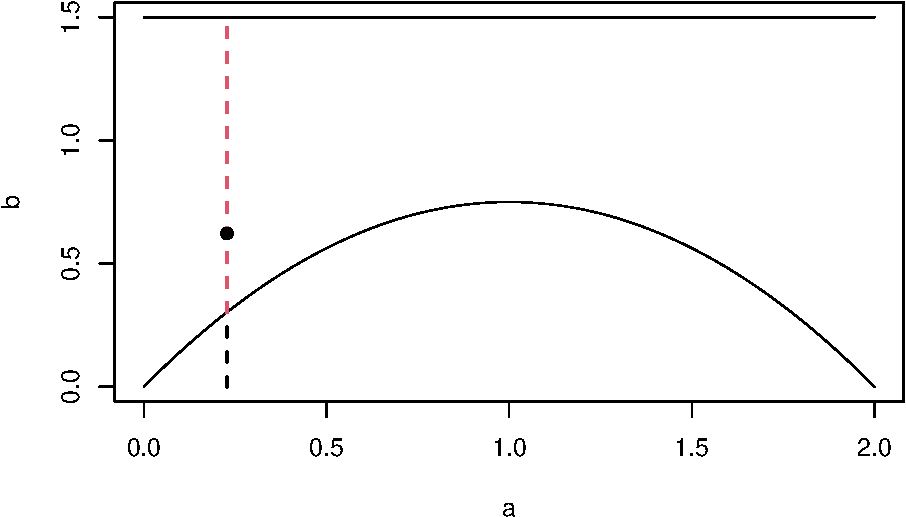
\includegraphics{_main_files/figure-latex/unnamed-chunk-26-1.pdf}
The plot also shows how the choices of \(c\) and \(q\) can make the sampling more or less efficient. In our example, the rejection space is large, meaning many of our proposed samples will be rejected. Here, we could have chosen a better \(q\) to minimise this space.
\end{example}

\begin{example}

Suppose we want to sample from a Beta(4, 8) distribution. This distribution looks like

\begin{Shaded}
\begin{Highlighting}[]
\NormalTok{x }\OtherTok{\textless{}{-}} \FunctionTok{seq}\NormalTok{(}\DecValTok{0}\NormalTok{, }\DecValTok{1}\NormalTok{, }\FloatTok{0.001}\NormalTok{)}
\NormalTok{y }\OtherTok{\textless{}{-}} \FunctionTok{dbeta}\NormalTok{(x, }\DecValTok{4}\NormalTok{, }\DecValTok{8}\NormalTok{)}
\end{Highlighting}
\end{Shaded}

A uniform distribution on {[}0, 1{]} will cover the Beta distribution and we can then use a rejection sampling algorithm. First, we need to find \(c\), the maximum of the Beta distribution. We can find this by differentiating the pdf and setting it equal to 0:
\[
\pi(x) = \frac{1}{B(4, 8)}x^3(1-x)^7 \\
\implies \frac{d \pi(x)}{d x} = \frac{1}{B(4, 8)}(3x^2(1-x)^7 - 7x^3(1-x)^6) \\
\implies \frac{d \pi(x)}{d x} = \frac{1}{B(4, 8)}(x^2(1-x)^7(3-10x)).
\]
Setting this equal to 0 gives us the maximum at \(x = \frac{3}{10}\). This means we can set \(\pi(3/10) = \frac{1}{B(4, 8)} \frac{3^7 7^{10}}{10^{10}}\). Our rejection sampling algorithm is therefore

\begin{enumerate}
\def\labelenumi{\arabic{enumi}.}
\tightlist
\item
  Sample \(u \sim U[0, 1]\)
\item
  Compute \(k = \pi(u)/cq(u)\).
\item
  Accept \(u\) with probability \(k\).
\end{enumerate}

\end{example}

\begin{example}

In this example, we want to sample from a Gamma(3, 2) distribution. The density function is shown below.

\begin{Shaded}
\begin{Highlighting}[]
\NormalTok{x }\OtherTok{\textless{}{-}} \FunctionTok{seq}\NormalTok{(}\DecValTok{0}\NormalTok{, }\DecValTok{6}\NormalTok{, }\FloatTok{0.01}\NormalTok{)}
\NormalTok{y }\OtherTok{\textless{}{-}} \FunctionTok{dgamma}\NormalTok{(x, }\DecValTok{3}\NormalTok{, }\DecValTok{2}\NormalTok{)}
\end{Highlighting}
\end{Shaded}

We will use an Exp(1) distribution as our proposal distribution. To find the value of \(c\), consider \(R(x) = \frac{\pi(x)}{q(x)}\)
\[
R(x) = \frac{\frac{2^3}{\Gamma(3)}x^2\exp(-2x)}{\exp(-x)} \\
 =  \frac{2^3}{\Gamma(3)}x^2 \exp(-x)
\]
To find the maximum of this ratio, we differentiate and set the result equal to 0.
\[
\frac{dR}{dx} = 2x\exp(-x) - x^2\exp(-x)\\
= x\exp(-x)(2 - x)
\]
The maximum is therefore at 2. The value of the ratio at \(x = 2\) is \(R(2) = \frac{2^3}{\Gamma(3)}4\exp(-2)\). This is therefore our value of c.~We can see how \(\pi(x)\) and \(cq(x)\) look of the graph below.

\begin{Shaded}
\begin{Highlighting}[]
\NormalTok{x }\OtherTok{\textless{}{-}} \FunctionTok{seq}\NormalTok{(}\DecValTok{0}\NormalTok{, }\DecValTok{6}\NormalTok{, }\FloatTok{0.01}\NormalTok{)}
\NormalTok{y }\OtherTok{\textless{}{-}} \FunctionTok{dgamma}\NormalTok{(x, }\DecValTok{3}\NormalTok{, }\DecValTok{2}\NormalTok{)}
\NormalTok{scaling.c }\OtherTok{\textless{}{-}} \DecValTok{2}\SpecialCharTok{\^{}}\DecValTok{3}\SpecialCharTok{/}\FunctionTok{gamma}\NormalTok{(}\DecValTok{3}\NormalTok{)}\SpecialCharTok{*}\DecValTok{4}\SpecialCharTok{*}\FunctionTok{exp}\NormalTok{(}\SpecialCharTok{{-}}\DecValTok{2}\NormalTok{)}
\NormalTok{q }\OtherTok{\textless{}{-}} \FunctionTok{dexp}\NormalTok{(x, }\DecValTok{1}\NormalTok{)}

\FunctionTok{plot}\NormalTok{(x, y, }\AttributeTok{type =} \StringTok{\textquotesingle{}l\textquotesingle{}}\NormalTok{)}
\FunctionTok{lines}\NormalTok{(x, q}\SpecialCharTok{*}\NormalTok{scaling.c, }\AttributeTok{col =} \DecValTok{2}\NormalTok{, }\AttributeTok{lty =} \DecValTok{2}\NormalTok{)}
\end{Highlighting}
\end{Shaded}

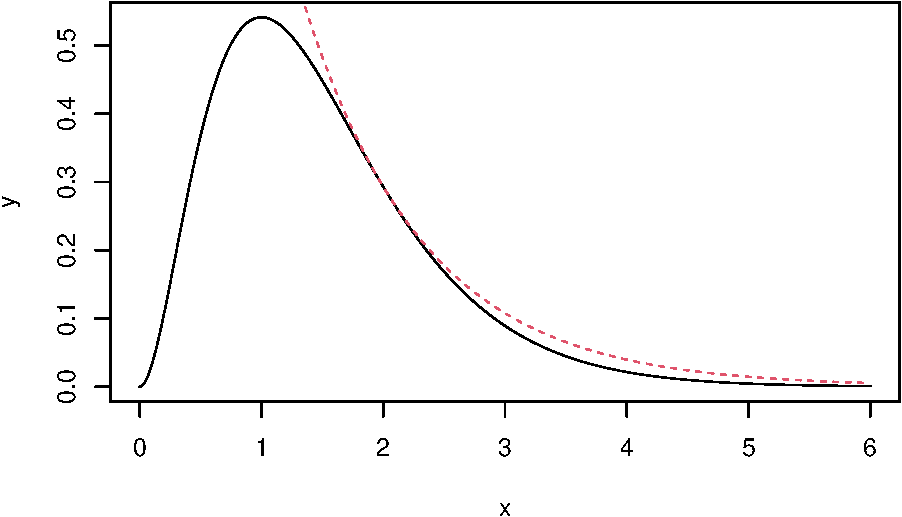
\includegraphics{_main_files/figure-latex/unnamed-chunk-29-1.pdf}

The exponential distribution completely encloses the gamma distribution using this value of \(c\), wiht the two densities just touching at \(x=2\). Our rejection sampling algorithm is therefore

\begin{enumerate}
\def\labelenumi{\arabic{enumi}.}
\tightlist
\item
  Sample \(u \sim \hbox{exp}(1)\)
\item
  Compute \(k = \frac{\pi(u)}{cq(u)}\)
\item
  Accept \(u\) with probability \(k\).
\end{enumerate}

\end{example}

\hypertarget{rejection-sampling-efficiency}{%
\subsection{Rejection Sampling Efficiency}\label{rejection-sampling-efficiency}}

Suppose we are using a rejection sampling algorithm to sample from \(f(y)\) using the proposal distribution \(g(y)\). How good is our rejection sampling algorithm? What does it mean to be a `good' rejection sampling algorithm. One measure of the efficiency of a sampler is, on average, how many samples to we need to generate until one is accepted.

\begin{proposition}
The number of samples proposed in a rejection sampling algorithm before one is accepted is distributed geometrically with mean \(\frac{1}{M}\).
\end{proposition}

\begin{proof}
Given a proposed value \(y\), and let \(A\) be the event of sample is accepted. The probability a sample is accepted, given it takes the value \(y\) is
\[
A \mid y \sim \hbox{Bernoulli}\left(\frac{f(y)}{Mg(y)}\right).
\]

By the tower property
\begin{align*}
E(A) & = E(E(A\mid y)) \\
& = E\left(\frac{f(y)}{Mg(y)}\right) \\
& = \int \frac{f(y)}{Mg(y)} g(y) dy \\
& = \frac{1}{M}\int f(y) dy \\
& = \frac{1}{M}.
\end{align*}

Therefore, the number of samples proposed before one is accepted is distributed geometrically with mean \(\frac{1}{M}\).
\end{proof}

\hypertarget{ziggurat-sampling}{%
\section{Ziggurat Sampling}\label{ziggurat-sampling}}

The final method we are going to look at in this chapter is Ziggurat sampling. It is used to sample from a \(N(0, 1)\) distribution using samples from a \(U(0, 1)\) distribution. A Ziggurat is a kind of stepped pyramid. To start the sampling algorithm, we approximate the normal distribution by a series of horizontal rectangles, each with the same area. An example of this is shown below.

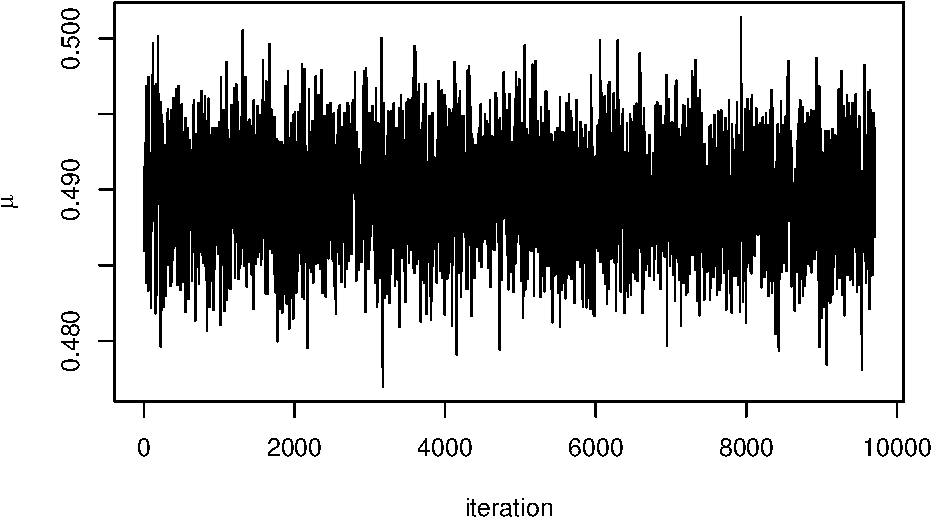
\includegraphics{_main_files/figure-latex/unnamed-chunk-30-1.pdf}
To generate a sample, we choose a rectangle at random -- we might do this by sampling on the y-axis uniformly at random. We then sample uniformly at random within the rectangle. We accept the sample if it is `clearly' in the box. By clearly, we mean that is is also contained in the rectangle above. If it is, not contained in the rectangle above, we generate a new uniform random number to accept or reject the sample.

Suppose the bottom right corner of the \(i^{th}\) rectangle has coordinates \((x_i, y_i)\). The Ziggurat algorithm is

\begin{enumerate}
\def\labelenumi{\arabic{enumi}.}
\tightlist
\item
  Sample a rectangle \(i\) uniformly at random
\item
  Sample \(u_0 \sim U[0, 1]\) and set \(x = u_0x_i\)
\item
  If \(x < x_{i+1}\) accept the sample
\item
  Sample \(u_1 \sim U[0, 1]\) and set \(y = y_i + u_1(y_{i+1} − y_i)\)
\item
  If \(y < f(y)\), where \(f\) is the density function of a standard normal distribution, then accept the sample.
\end{enumerate}

This only generates samples for the positive side of the normal distribution. To generate samples from the full distribution, we multiply each sample by -1 with probability a half.

\hypertarget{lab-1}{%
\section{Lab}\label{lab-1}}

The aim of this lab is to code up some sampling methods. You have already done some similar work in lab 1 (e.g.~estimating \(\pi\)).

\begin{exercise}
Visit random.org to generate some truly random numbers. How does this site generate numbers that are truly random?
\end{exercise}

\begin{exercise}
A random variable \(X\) has density \(\pi(x) = ax^2\) for \(x\in[0,1]\) and 0 otherwise. Find the value \(a\). Use the inverse transform method to generate 10,000 samples from this distribution. Plot a histogram against the true density function.
\end{exercise}

\begin{exercise}
Let \(X\) have the density \(\pi(x) = \frac{1}{\theta}x^{\frac{1-\theta}{\theta}}\) for \(x \in [0, 1]\). Use the inverse transform method to generate 10,000 samples from this distribution with \(\theta = \{1, 5, 10\}\).
\end{exercise}

\begin{exercise}
Let \(X\) have the density \(\pi(x) = 3x^2\) for \(x \in [0, 1]\) and 0 otherwise. Use a rejection sampling method to generate 10,000 from this distribution. Plot the results against the true density to check you have the same distribution.
\end{exercise}

\begin{exercise}

The half normal distribution with mean 0 and variance 1 has density function
\[
\pi(x) = \frac{2}{\sqrt{2\pi}}\exp{(-x^2/2)}
\]
for \(x \geq 0\) and 0 otherwise.

\begin{enumerate}
\def\labelenumi{\arabic{enumi}.}
\tightlist
\item
  Denote the exponential density function by \(q(x) = \lambda \exp(-\lambda x)\). Find the smallest \(c\) such that \(\pi(x)/q(x) < c\).
\item
  Use a rejection sampling algorithm with an exponential proposal distribution to generate samples from the half normal distibrution with mean 0 and variance 1.
\end{enumerate}

\end{exercise}

\hypertarget{markov-chain-monte-carlo}{%
\chapter{Markov Chain Monte Carlo}\label{markov-chain-monte-carlo}}

Markov Chain Monte Carlo (MCMC) is a class of algorithms that produce samples from a probability distribution. These methods combine the idea of rejection sampling with the theory of Markov chains. Before we set out the theory of Markov chains, we'll go through an example to show how MCMC works.

\begin{example}
\protect\hypertarget{exm:King}{}\label{exm:King}(\href{https://xcelab.net/rm/statistical-rethinking/}{Adapted from Statistical Rethinking \S 9}) Consider an eccentric King whose kingdom consists of a ring of 10 islands. Directly north is island one, the smallest island. Going clockwise around the archipelago, next is island two, which is twice the size of island one, then island three, which is three times as large as island one. Finally, island 10 is next to island one and ten times as large.

The King wanted to visit all of his islands, but spending time on each one according to its size. That is he should spend the most time on island ten and the least on island one. Being climate conscious, he also decided that flying from one side of the archipelago to the other was not allowed. Instead, he would only sail from one island to either of its neighbors. So from island one, he could reach islands two and ten.

He decided to travel according to these rules:

\begin{enumerate}
\def\labelenumi{\arabic{enumi}.}
\item
  At the end of each week, he decides to stay on the same island or move to a neighboring island according to a coin toss. If it's heads he proposes moving clockwise, and tails anti-clockwise. The island he is considering moving to is called the proposal island.
\item
  To decided if he is going to move to the proposal island, the King counts out a number of shells equal to the number of size of the island. So if island five is the proposal island, he counts out five shells. He then counts out a number of stones equal to the size of the current island.
\item
  If the number of seashells is greater than the number of stones, he moves to the proposed island. If the number of seashells is less than the number of stones, he takes a different strategy. He discards the number of stones equal to the number of seashells. So if there are six stone and five seashells, he ends up with 6-5=1 stones. He then places the stones and seashells into a bag a chooses one at random. If he picks a seashell, he moves to the proposed island, otherwise if he picks a shell, he stays put.
\end{enumerate}

This is a complex way of moving around, but it produces the required result; the time he spends on each island is proportionate to the size of the island. The code below shows an example of this over 10,000 weeks.

\begin{Shaded}
\begin{Highlighting}[]
\NormalTok{weeks }\OtherTok{\textless{}{-}} \DecValTok{10000}
\NormalTok{island }\OtherTok{\textless{}{-}} \FunctionTok{numeric}\NormalTok{(weeks)}
\NormalTok{current }\OtherTok{\textless{}{-}} \DecValTok{10}
\ControlFlowTok{for}\NormalTok{(i }\ControlFlowTok{in} \DecValTok{1}\SpecialCharTok{:}\NormalTok{weeks)\{}
  \DocumentationTok{\#\# record current position}
\NormalTok{  island[i] }\OtherTok{\textless{}{-}}\NormalTok{ current}
  
  \CommentTok{\#Flip a coin to move to a propose a new island}
\NormalTok{  proposed }\OtherTok{\textless{}{-}}\NormalTok{ current }\SpecialCharTok{+} \FunctionTok{sample}\NormalTok{(}\FunctionTok{c}\NormalTok{(}\DecValTok{1}\NormalTok{, }\SpecialCharTok{{-}}\DecValTok{1}\NormalTok{), }\AttributeTok{size =} \DecValTok{1}\NormalTok{)}
  
  \CommentTok{\#Ensure he loops round the island}
  \ControlFlowTok{if}\NormalTok{(proposed }\SpecialCharTok{\textless{}} \DecValTok{1}\NormalTok{) }
\NormalTok{    proposed }\OtherTok{\textless{}{-}} \DecValTok{10}
  \ControlFlowTok{if}\NormalTok{(proposed }\SpecialCharTok{\textgreater{}} \DecValTok{10}\NormalTok{)}
\NormalTok{    proposed }\OtherTok{\textless{}{-}} \DecValTok{1}
  
  \CommentTok{\#Decide to move}
\NormalTok{  p }\OtherTok{\textless{}{-}}\NormalTok{ proposed}\SpecialCharTok{/}\NormalTok{current}
\NormalTok{  u }\OtherTok{\textless{}{-}} \FunctionTok{runif}\NormalTok{(}\DecValTok{1}\NormalTok{)}
  \ControlFlowTok{if}\NormalTok{(u }\SpecialCharTok{\textless{}}\NormalTok{ p)}
\NormalTok{    current }\OtherTok{\textless{}{-}}\NormalTok{ proposed}
\NormalTok{\}}

\CommentTok{\#Plot results}
\FunctionTok{plot}\NormalTok{(island, }\AttributeTok{type =} \StringTok{\textquotesingle{}l\textquotesingle{}}\NormalTok{, }\AttributeTok{xlab =} \StringTok{"Week"}\NormalTok{, }\AttributeTok{ylab =} \StringTok{"Island"}\NormalTok{)}
\end{Highlighting}
\end{Shaded}

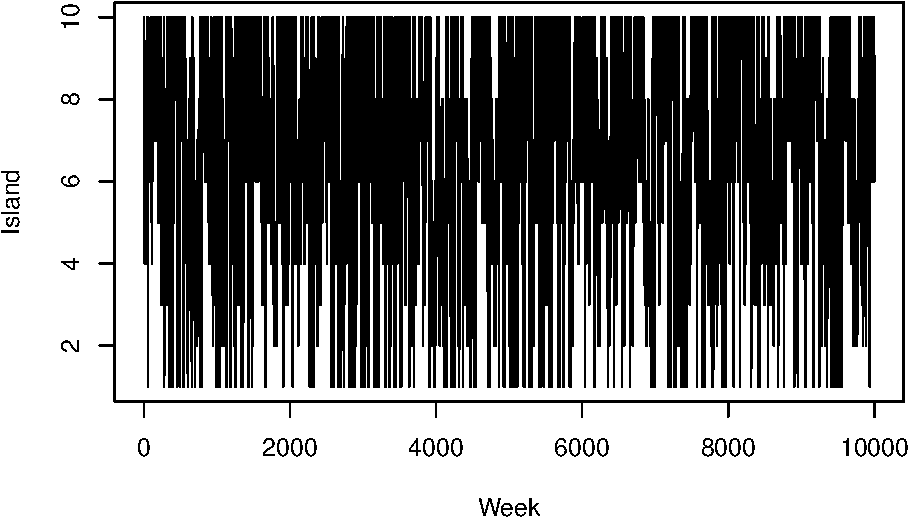
\includegraphics{_main_files/figure-latex/unnamed-chunk-31-1.pdf}

\begin{Shaded}
\begin{Highlighting}[]
\FunctionTok{barplot}\NormalTok{(}\FunctionTok{table}\NormalTok{(island)}\SpecialCharTok{/}\NormalTok{weeks, }\AttributeTok{xlab =} \StringTok{"Island"}\NormalTok{, }
        \AttributeTok{ylab =} \StringTok{"Proportion of time"}\NormalTok{)}
\end{Highlighting}
\end{Shaded}

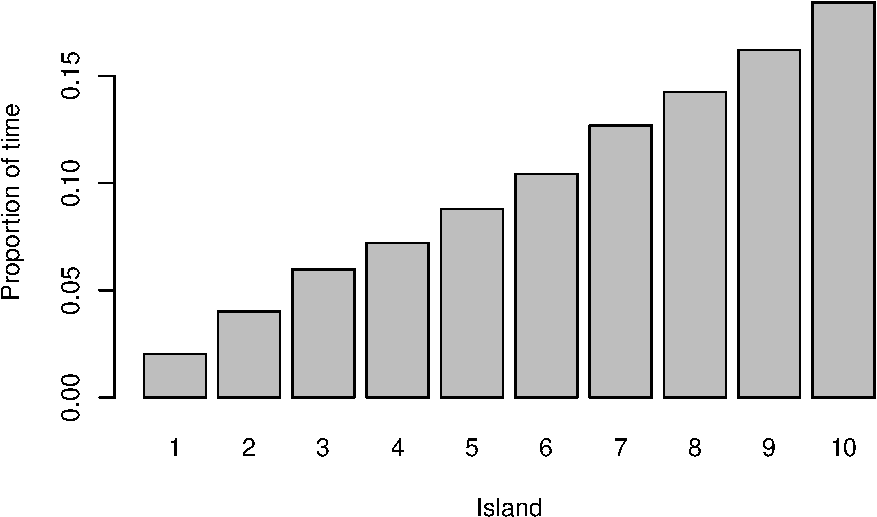
\includegraphics{_main_files/figure-latex/unnamed-chunk-31-2.pdf}
\end{example}

We can recognise several different statistical principles in this example. The King decides to move islands dependent on where he is currently, not based on where he has been previously (Markov property). He proposes an island to move to and accepts or rejects this decision based on some distribution (rejection principle). We are now going to describe some of the properties of Markov chains, including the Markov property.

\hypertarget{properties-of-markov-chains}{%
\section{Properties of Markov Chains}\label{properties-of-markov-chains}}

\begin{definition}
\protect\hypertarget{def:Markov}{}\label{def:Markov}A sequence of random variables \(\{Y_1, Y_2, \ldots\}\) is a \textbf{Markov chain} if \(\mathbb{P}(Y_{n+1} \mid Y_{n}, \ldots, Y_1) = \mathbb{P}(Y_{n+1} \mid Y_{n})\). That is that distribution of the next state \(Y_{n+1}\) only depends on the current state \(Y_n\) and not any previous states.
\end{definition}

\begin{definition}
The probability of transitioning from state \(i\) to state \(j\) in a Markov chain is given by \(p_{ij}\). The \textbf{transition matrix} for a Markov chain with \(N\) states is the \(N \times N\) matrix \(P\), where the \(\{i, j\}^{th}\) entry denoted by \(p_{ij}\) is probability is moving from state \(i\) to state \(j\).
\end{definition}

These two properties make Markov chains nice to work with, especially the Markov property (Definition \ref{def:Markov}). Two other important definitions are

\begin{definition}
The \textbf{period }of a state \(i\) is given by \(d_i = \textrm{gcd}\{n > 0; p_{ii} > 0 \}\). A state is \textbf{aperiodic} if \(d_i = 1\). An \textbf{aperiodic chain} is a chain where all states are aperiodic.
\end{definition}

\begin{definition}
A Markov chain is \textbf{irreducible} if there exists an \(n \in \mathbb{N}\) such that \(\mathbb{P} (Y_n = i \mid Y_0 = j) > 0\) for all pairs \(i\) and \(j\). In other words, it is possible to move from any state to any other state in a finite number of steps.
\end{definition}

We can use these definitions to start working with distributions. Suppose, the state we start at is drawn from some distribution \(Y_1 \sim \boldsymbol{q}\). Then the distributions of the second state \(Y_2\) depends on the distribution of \(Y_1\) and the transition probabilities
\[
\mathbb{P}(Y_2 = j) = \sum_i q_ip_{ij}.
\]
If we denote the distribution of \(Y_2 \sim \boldsymbol{q}^{(2)}\), then we can write it in terms of the transition matrix \(\boldsymbol{q}^\prime = \boldsymbol{q}P\). Now suppose we would like the distribution of \(Y_3 \sim \boldsymbol{q}^{(3)}\), thanks to the Markov property, this is the distribution for \(Y_2\) multiplied by the transition matrix, so \(Y_3 \sim qP^2\). Inductively, \(P_k \sim qP^{k-1}\). To use Markov chains to sample from distributions, we need to identify the Eigenvalues of the transition matrix.

\begin{proposition}
A transition matrix \(P\) always has at least one eigenvalue equal to one.
\end{proposition}

\begin{proof}
The columns of \(P\) sum to 1 as they are probability distributions. Therefore, \(1\) is an eigenvalue.
\end{proof}

\begin{definition}
If a transition matrix \(P\) has a unique Eigenvalue that takes the value 1, there is a unique distribution \(\pi\) such that
\[
\pi P = \pi. 
\]
This distribution \(\pi\), is known as the \textbf{stationary distribution}.
\end{definition}

This important concept underpins MCMC methods. It says that no matter where we start our chain, we'll eventually end up sampling states according to the distribution \(\pi\). It make take a long time to reach the stationary distribution, but it will eventually get there.

In order to check whether our Markov chain will converge to a stationary distribution, we need to check:

\begin{enumerate}
\def\labelenumi{\arabic{enumi}.}
\item
  the Markov chain is aperiodic,
\item
  the Markov chain is irreducible, and
\item
  that there exists a unique distribution \(\pi\) such that \(\pi P = \pi\).
\end{enumerate}

\begin{example}
In Example \ref{exm:King}, the King wanted to visit the islands according to how large they are. We can think of the islands as the states and the stationary distribution as \(p(Y = i) \propto i\). The eccentric method the King used allowed him to construct a transition matrix for an aperiodic Markov chain. He also never visited islands regularly using this method.
\end{example}

When designing a Markov chain, it is usually straightforward to design one that meets conditions one and two. Condition three is more difficult to prove, but for some chains it is possible to show they satisfy detailed balance.

\begin{definition}
The Markov chain with transition matrix \(P\) satisfies the \textbf{detailed balance} equation with respect to the distribution \(\pi\) if
\[
\pi_i p_{ij} = \pi_j p_{ji}. 
\]
\end{definition}

\begin{theorem}[Detailed Balance]
Let \(P\) be a transition matrix that satisfies detailed balance with respect to the distribution \(\pi\). Then \(\pi P = \pi\).
\end{theorem}

\begin{proof}
The \(j^{th}\) row of \(\pi P\) is
\begin{align*}
\sum_{i} \pi_i p_{ij} & = \sum_{i} \pi_j p_{ji} \quad \textrm{(detailed balance)} \\
 & = \pi_j \sum_{i} p_{ji} \\
 & = \pi_j.\qquad \textrm{(probaility sums to 1)}
\end{align*}
Hence \(\pi P = \pi\).
\end{proof}

The section has shown us that we can use a Markov chain theory to simulate from a probability distribution \(\pi\). All we need is for the Markov chain to be irreducible, aperiodic, and for the transition matrix to satisfy \(\pi P = \pi\). This provides the foundation theory for MCMC and allows us to sample from a posterior distribution \(\pi\). What it doesn't tell us is how to design the Markov chain, and that is what the next sections deal with.

\hypertarget{metropolis-hastings}{%
\section{Metropolis-Hastings}\label{metropolis-hastings}}

We're now going to look at MCMC algorithms. The first algorithm we are going to look at is the Metropolis-Hasting algorithm. This is a useful algorithm if we cannot sample directly from the posterior distribution and if the conditional distributions do not have a closed form. The Metropolis-Hastings algorithm is like the island example we saw earlier. At each iteration, we propose a new sample and then accept or reject it based on the likelihood function, the prior and how likely we are to propose this new sample given the current one.

Suppose we want to sample from the posterior distribution \(\pi(\theta \mid \boldsymbol{y})\). The Metropolis-Hastings works as follows:

\begin{enumerate}
\def\labelenumi{\arabic{enumi}.}
\item
  Set the initial value \(\theta^{(0)}\).
\item
  Set \(i = 1\).
\item
  Propose a new value of \(\theta'\) from some distribution \(q\)
\item
  Accept \(\theta' = \theta^{(i)}\) with probability
  \[
  p_{\textrm{acc}} = \min\left\{\frac{\pi(\theta' \mid \boldsymbol{y})}{\pi(\theta \mid \boldsymbol{y})}\frac{q(\theta \mid \theta')}{q(\theta' \mid \theta)}, 1\right\}.
  \]
\item
  Set \(i = i+1\) and repeat steps 3 to 4 for \(i = 2, \ldots, M\).
\end{enumerate}

There are two parts to the acceptance probability in step 4. The first is the posterior ratio, similar to saying the likelihood of \(\theta'\) given the observed data over the likelihood of \(\theta\) given the data. The second is the proposal ratio. It is similar to saying the likelihood of proposing \(\theta\) given the current value \(\theta'\), over the likelihood of proposing \(\theta'\) given the current value \(\theta\).

In practice, we don't need to evaluate the full posterior distribution. Recall
\[
\pi(\theta \mid \boldsymbol{y}) = \frac{\pi(\boldsymbol{y} \mid \theta) \pi(\theta)}{\pi(y)}
\]
As the the denominator doesn't depend on \(\theta\), it cancels in the ration. The ratio becomes
\[
\frac{\pi(\theta' \mid \boldsymbol{y})}{\pi(\theta \mid \boldsymbol{y})} = \frac{\pi(\boldsymbol{y} \mid \theta') \pi(\theta')}{\pi(\boldsymbol{y} \mid \theta) \pi(\theta)}.
\]
This is the likelihood ratio multiplied by the prior ratio.

\begin{proposition}
The Markov chain generated by the Metropolis-Hastings algorithm satisfies detailed balance with respect to the posterior distribution.
\end{proposition}

\begin{proof}
Denote the current state \(\theta\) and the proposed state \(\theta'\). We would like to show
\[
\pi(\theta \mid \boldsymbol{y}) \pi(\theta'\mid\theta) = \pi(\theta' \mid \boldsymbol{y}) \pi(\theta\mid\theta').
\]
The density of \(\theta'\) given the proposed state \(\theta\) is the proposal density multiplied by the acceptance probability. It is given by
\begin{align*}
\pi(\theta' \mid \theta) &= q(\theta' \mid \theta)p_{acc}\\
&=  q(\theta' \mid \theta)\min\left\{\frac{\pi(\theta' \mid \boldsymbol{y})}{\pi(\theta' \mid \boldsymbol{y})}\frac{q(\theta \mid \theta')}{q(\theta' \mid \theta)}, \, 1\right\} \\
& = \min\left\{\frac{\pi(\theta' \mid \boldsymbol{y})}{\pi(\theta' \mid \boldsymbol{y})}q(\theta \mid \theta'),\, q(\theta' \mid \theta)\right\}.
\end{align*}

The left hand side of the detailed balance equation becomes
\[
\pi(\theta \mid \boldsymbol{y})\pi(\theta' \mid \theta) = \min\{\pi(\theta' \mid \boldsymbol{y})q(\theta \mid \theta'),\, \pi(\theta \mid \boldsymbol{y})q(\theta' \mid \theta)\}.
\]
Analogously, we can show the right hand side is

\[
\pi(\theta' \mid \boldsymbol{y})\pi(\theta \mid \theta') = \min\{\pi(\theta' \mid \boldsymbol{y})q(\theta \mid \theta'),\, \pi(\theta \mid \boldsymbol{y})q(\theta' \mid \theta)\}.
\]
Hence, \(\pi(\theta \mid \boldsymbol{y}) \pi(\theta'\mid\theta) = \pi(\theta' \mid \boldsymbol{y}) \pi(\theta\mid\theta')\) and the Markov chain satisfies detailed balance with respect to the posterior disquisition.
\end{proof}

\begin{example}
\protect\hypertarget{exm:norm}{}\label{exm:norm}

A counter monitors the time until atoms decays. It collects the data \(X_1, \ldots, X_N\) and we assume \(X_i \sim \hbox{Exp}(\lambda)\). The time until these atom decays is short, less than 1 second, so we assume \(\lambda \sim \hbox{Beta}(\alpha, \beta)\).

The prior distribution is given by
\[
\pi(\lambda \mid \boldsymbol{x}) \propto \lambda^{N + \alpha - 1} (1 - \lambda)^{\beta - 1}\exp\left(-\lambda \sum x_i\right)
\]
This doesn't have a closed form, so we need to use a Metropolis-Hastings algorithm to generate samples from this distribution. A suitable algorithm is

\begin{enumerate}
\def\labelenumi{\arabic{enumi}.}
\tightlist
\item
  Decide on an starting value the Markov chain and denote it \(\lambda^{(1)}\). Set \(i = 1\).
\item
  Propose a new value for the parameter and denote it \(\lambda'\). In this example, we are going to propose values using a random walk method where \(\lambda' \sim N(\lambda^{(i)}, \sigma^2)\).
\item
  Accept \(\lambda'\) as the value \(\lambda^{(i+1)}\) with probability \(p_{\textrm{acc}}\). Otherwise reject this value and set \(\lambda^{(i+1)} = \lambda^{(i)}\).\\
\item
  Set \(i = i + 1\).
\item
  Repeat steps 2, 3, 4, for \(i = 2, \ldots, M\).
\end{enumerate}

The value \(p_{\textrm{acc}}\) is given by
\[
p_{\textrm{acc}} = \min \left\{1, \, \frac{\lambda'^{N + \alpha - 1} (1 - \lambda')^{\beta - 1}\exp\left(-\lambda' \sum x_i\right)}{\lambda^{N + \alpha - 1} (1 - \lambda)^{\beta - 1}\exp\left(-\lambda \sum x_i\right)}\right\} \\
= \min \left\{1, \, \left(\frac{\lambda'}{\lambda}\right)^{N + \alpha - 1} \left(\frac{1-\lambda'}{1-\lambda}\right)^{\beta -1} \exp\left((\lambda- \lambda')\sum x\right)\right\} 
\]
As we our proposal distribution is symmetric, \(q(\lambda \mid \lambda') = q(\lambda' \mid \lambda)\) and this term cancels.

The code below shows this algorithm in action

\begin{Shaded}
\begin{Highlighting}[]
\CommentTok{\# Set Up MCMC Algorithm {-}{-}{-}{-}{-}{-}{-}{-}{-}{-}{-}{-}{-}{-}{-}{-}{-}{-}{-}{-}{-}{-}{-}{-}{-}{-}{-}{-}{-}{-}{-}{-}{-}{-}{-}{-}{-}{-}{-}{-}{-}{-}{-}{-}{-}{-}{-}{-}{-}{-}{-}}

\NormalTok{n.iter }\OtherTok{\textless{}{-}} \DecValTok{10000}
\NormalTok{lambda.store }\OtherTok{\textless{}{-}} \FunctionTok{numeric}\NormalTok{(n.iter) }\CommentTok{\#Store value of Markov chain at end of every iteration}

\CommentTok{\#Initialise Prior Parameters and Data}
\NormalTok{lambda }\OtherTok{\textless{}{-}} \FloatTok{0.5}
\NormalTok{sum.x }\OtherTok{\textless{}{-}} \FloatTok{67.6}
\NormalTok{N }\OtherTok{\textless{}{-}} \DecValTok{20}
\NormalTok{alpha }\OtherTok{\textless{}{-}} \DecValTok{1}
\NormalTok{beta }\OtherTok{\textless{}{-}} \DecValTok{1}


\CommentTok{\# Run MCMC Algorithm {-}{-}{-}{-}{-}{-}{-}{-}{-}{-}{-}{-}{-}{-}{-}{-}{-}{-}{-}{-}{-}{-}{-}{-}{-}{-}{-}{-}{-}{-}{-}{-}{-}{-}{-}{-}{-}{-}{-}{-}{-}{-}{-}{-}{-}{-}{-}{-}{-}{-}{-}{-}{-}{-}}
\ControlFlowTok{for}\NormalTok{(i }\ControlFlowTok{in} \DecValTok{1}\SpecialCharTok{:}\NormalTok{n.iter)\{}
  
  \CommentTok{\#Propose new value of lambda}
\NormalTok{  lambda.prop }\OtherTok{\textless{}{-}} \FunctionTok{rnorm}\NormalTok{(}\DecValTok{1}\NormalTok{, lambda, }\FloatTok{0.1}\NormalTok{)}
  
  \CommentTok{\#Check lambda \textbackslash{}in [0, 1]}
  \ControlFlowTok{if}\NormalTok{(lambda.prop }\SpecialCharTok{\textgreater{}} \DecValTok{0} \SpecialCharTok{\&}\NormalTok{ lambda.prop }\SpecialCharTok{\textless{}} \DecValTok{1}\NormalTok{)\{}
    
    \CommentTok{\#Compute p\_acc}
\NormalTok{    log.p.acc }\OtherTok{\textless{}{-}}\NormalTok{ (N }\SpecialCharTok{+}\NormalTok{ alpha }\SpecialCharTok{{-}} \DecValTok{1}\NormalTok{)}\SpecialCharTok{*}\FunctionTok{log}\NormalTok{(lambda.prop}\SpecialCharTok{/}\NormalTok{lambda) }\SpecialCharTok{+} 
\NormalTok{      (beta }\SpecialCharTok{{-}} \DecValTok{1}\NormalTok{)}\SpecialCharTok{*}\FunctionTok{log}\NormalTok{((}\DecValTok{1}\SpecialCharTok{{-}}\NormalTok{lambda.prop)}\SpecialCharTok{/}\NormalTok{(}\DecValTok{1}\SpecialCharTok{{-}}\NormalTok{lambda)) }\SpecialCharTok{+}
\NormalTok{      (lambda }\SpecialCharTok{{-}}\NormalTok{ lambda.prop)}\SpecialCharTok{*}\NormalTok{sum.x}
    
    \CommentTok{\#Accept/Reject step}
    \ControlFlowTok{if}\NormalTok{(}\FunctionTok{log}\NormalTok{(}\FunctionTok{runif}\NormalTok{(}\DecValTok{1}\NormalTok{)) }\SpecialCharTok{\textless{}}\NormalTok{ log.p.acc)}
\NormalTok{      lambda }\OtherTok{\textless{}{-}}\NormalTok{ lambda.prop}
    
\NormalTok{  \}}
  
  \CommentTok{\#Store current value of Markov Chain}
\NormalTok{  lambda.store[i] }\OtherTok{\textless{}{-}}\NormalTok{ lambda}
  
\NormalTok{\}}

\CommentTok{\#Plot trace plot (Markov chain values)}
\FunctionTok{plot}\NormalTok{(lambda.store, }\AttributeTok{type =} \StringTok{\textquotesingle{}l\textquotesingle{}}\NormalTok{, }\AttributeTok{xlab =} \StringTok{"iteration"}\NormalTok{, }\AttributeTok{ylab =} \FunctionTok{expression}\NormalTok{(lambda))}
\FunctionTok{abline}\NormalTok{(}\AttributeTok{h=}\FloatTok{0.3}\NormalTok{, }\AttributeTok{col =} \DecValTok{2}\NormalTok{) }\CommentTok{\#the value I used to simulate the data}
\end{Highlighting}
\end{Shaded}

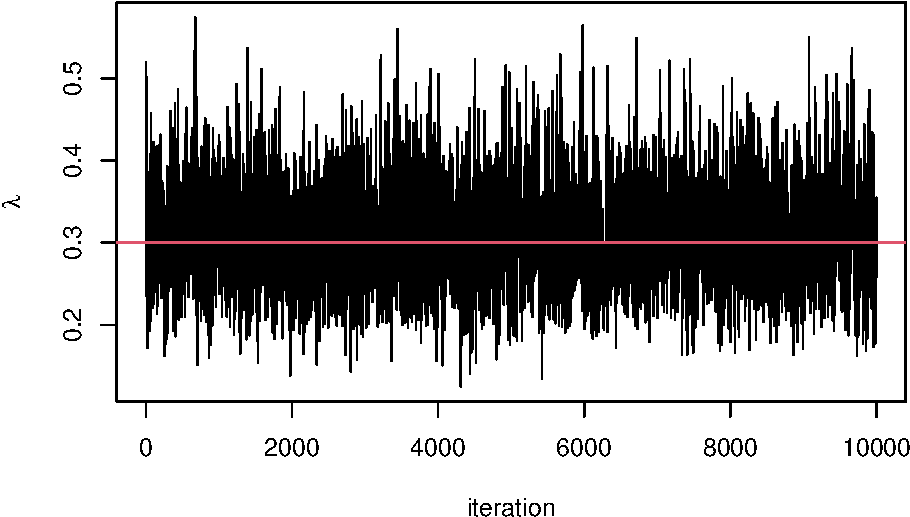
\includegraphics{_main_files/figure-latex/unnamed-chunk-32-1.pdf}

\begin{Shaded}
\begin{Highlighting}[]
\CommentTok{\#Plot posterior density}
\FunctionTok{hist}\NormalTok{(lambda.store, }\AttributeTok{prob =} \ConstantTok{TRUE}\NormalTok{, }\AttributeTok{xlab =} \FunctionTok{expression}\NormalTok{(lambda), }\AttributeTok{main =} \StringTok{"Posterior density"}\NormalTok{)}
\FunctionTok{abline}\NormalTok{(}\AttributeTok{v=}\FloatTok{0.3}\NormalTok{, }\AttributeTok{col =} \DecValTok{2}\NormalTok{) }\CommentTok{\#the value I used to simulate the data}
\end{Highlighting}
\end{Shaded}

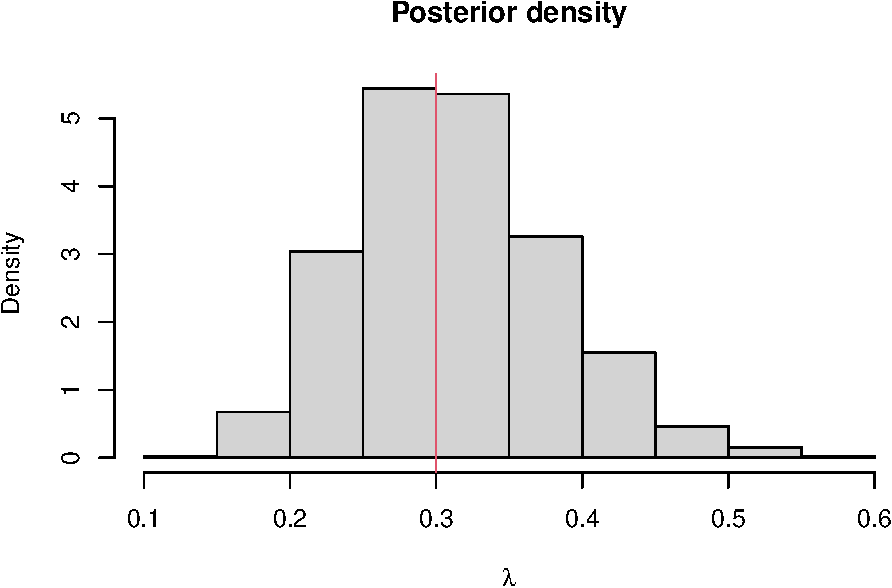
\includegraphics{_main_files/figure-latex/unnamed-chunk-32-2.pdf}

\begin{Shaded}
\begin{Highlighting}[]
\FunctionTok{mean}\NormalTok{(lambda.store) }\CommentTok{\#posterior mean}
\end{Highlighting}
\end{Shaded}

\begin{verbatim}
## [1] 0.3116649
\end{verbatim}

\begin{Shaded}
\begin{Highlighting}[]
\FunctionTok{quantile}\NormalTok{(lambda.store, }\FunctionTok{c}\NormalTok{(}\FloatTok{0.025}\NormalTok{, }\FloatTok{0.975}\NormalTok{)) }\CommentTok{\#95\% CI}
\end{Highlighting}
\end{Shaded}

\begin{verbatim}
##      2.5%     97.5% 
## 0.1937659 0.4582714
\end{verbatim}

\end{example}

\begin{example}
\protect\hypertarget{exm:norm}{}\label{exm:norm}The time until lorry drivers react (in milliseconds) to an obsticle in the road is

\begin{Shaded}
\begin{Highlighting}[]
\NormalTok{y }\OtherTok{\textless{}{-}} \FunctionTok{c}\NormalTok{(}\FloatTok{0.34}\NormalTok{, }\FloatTok{0.47}\NormalTok{, }\FloatTok{0.58}\NormalTok{, }\FloatTok{0.27}\NormalTok{, }\FloatTok{0.74}\NormalTok{, }\FloatTok{0.44}\NormalTok{, }\FloatTok{0.46}\NormalTok{, }\FloatTok{0.65}\NormalTok{, }\FloatTok{0.36}\NormalTok{, }\FloatTok{0.55}\NormalTok{, }\FloatTok{0.58}\NormalTok{, }\FloatTok{0.55}\NormalTok{, }
       \FloatTok{0.53}\NormalTok{, }\FloatTok{0.56}\NormalTok{, }\FloatTok{0.54}\NormalTok{, }\FloatTok{0.61}\NormalTok{, }\FloatTok{0.43}\NormalTok{, }\FloatTok{0.52}\NormalTok{, }\FloatTok{0.45}\NormalTok{, }\FloatTok{0.49}\NormalTok{, }\FloatTok{0.32}\NormalTok{, }\FloatTok{0.33}\NormalTok{, }\FloatTok{0.47}\NormalTok{, }\FloatTok{0.58}\NormalTok{, }
       \FloatTok{0.34}\NormalTok{, }\FloatTok{0.60}\NormalTok{, }\FloatTok{0.59}\NormalTok{, }\FloatTok{0.43}\NormalTok{, }\FloatTok{0.57}\NormalTok{, }\FloatTok{0.34}\NormalTok{)}
\FunctionTok{hist}\NormalTok{(y, }\AttributeTok{main =} \StringTok{""}\NormalTok{, }\AttributeTok{xlab =} \StringTok{"Reaction time (ms)"}\NormalTok{)}
\end{Highlighting}
\end{Shaded}

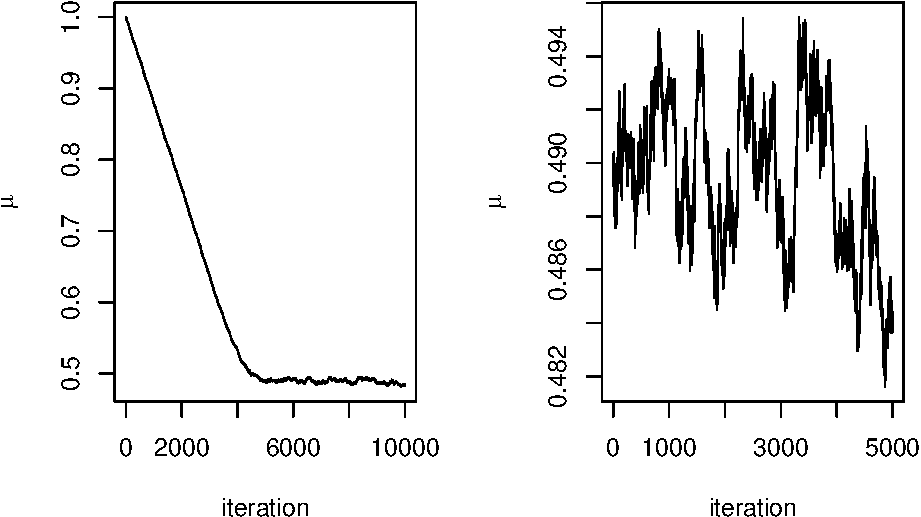
\includegraphics{_main_files/figure-latex/unnamed-chunk-33-1.pdf}

Assuming \(Y_i \sim N(\mu, \sigma^2)\) are independent and identically distributed for \(i=1,...,n\), by Bayes' theorem, the posterior distribution is

\[
\pi(\mu \mid \boldsymbol{y}, \sigma^2) \propto \pi(\boldsymbol{y} \mid \mu, \sigma^2) \pi(\mu).
\]
One of the issues here is that we have assigned a normal prior distribution to the population mean parameter \(\mu\). The advantage previously was that we could derive a posterior distribution with closed form. The disadvantage however is that the choice of prior distribution assigns some positive probability to impossible values of \(\mu\), i.e.~reaction times less than zero.

Now we have a tool to sample from posterior distributions that don't have a closed form. We can instead assign an exponential prior distribution, a distribution which only has non-negative support. Letting \(\mu \sim \textrm{Exp}(0.01)\) sets a vague prior distribution on \(\mu\). It can be shown that the posterior distribution (exercise) is therefore
\[
\pi(\mu \mid \boldsymbol{y}, \sigma^2) \propto \exp\left\{-0.01\mu -\sum_{i=1}^{30}\frac{(y_i - \mu)^2}{\sigma^2}\right\} 
\]

We can use the Metropolis-Hasting algorithm to sample from this posterior distribution. But how should we propose new value of \(\mu\)? A common method is a Metropolis-Hastings Random Walk proposal distribution. The proposal distribution is symmetric and centered on \(\mu\). The two most common methods are \(\mu' \mid \mu \sim U[\mu - \varepsilon, \mu + \varepsilon]\) and \(\mu' \mid \mu \sim N(\mu, \tau^2)\). We choose the uniform proposal distribution, with
\[
q(\mu' \mid \mu) = \frac{1}{2\varepsilon}.
\]

The acceptance probability is therefore
\[
p_\textrm{acc} = \min\left\{\frac{\exp\left\{-0.01\mu' -\sum_{i=1}^{30}\frac{(y_i - \mu')^2}{\sigma^2}\right\} }{\exp\left\{-0.01\mu -\sum_{i=1}^{30}\frac{(y_i - \mu)^2}{\sigma^2}\right\} }, 1\right\}
\]

We can implement a sampler in R as follows:

\begin{Shaded}
\begin{Highlighting}[]
\CommentTok{\#Set up elements for MCMC}
\FunctionTok{set.seed}\NormalTok{(}\DecValTok{123}\NormalTok{) }\CommentTok{\#to reproduce}
\NormalTok{n.iter   }\OtherTok{\textless{}{-}} \DecValTok{10000}
\NormalTok{mu.store }\OtherTok{\textless{}{-}} \FunctionTok{numeric}\NormalTok{(n.iter)}

\CommentTok{\#Initial values}
\NormalTok{mu }\OtherTok{\textless{}{-}} \DecValTok{1} 
\NormalTok{sigma }\OtherTok{\textless{}{-}} \FloatTok{0.1} \CommentTok{\#known}

\ControlFlowTok{for}\NormalTok{(i }\ControlFlowTok{in} \DecValTok{1}\SpecialCharTok{:}\NormalTok{n.iter)\{}
  
  \CommentTok{\#Propose value for mu}
\NormalTok{  mu.proposed }\OtherTok{\textless{}{-}} \FunctionTok{runif}\NormalTok{(}\DecValTok{1}\NormalTok{, mu }\SpecialCharTok{{-}} \FloatTok{0.01}\NormalTok{, mu }\SpecialCharTok{+} \FloatTok{0.01}\NormalTok{)}
  
  \ControlFlowTok{if}\NormalTok{(mu.proposed }\SpecialCharTok{\textgreater{}} \DecValTok{0}\NormalTok{)\{ }\CommentTok{\#If mu \textless{} 0 we can reject straight away}
    
    \CommentTok{\#Compute (log) acceptance probability}
\NormalTok{    log.numerator   }\OtherTok{\textless{}{-}} \SpecialCharTok{{-}}\FloatTok{0.01}\SpecialCharTok{*}\NormalTok{mu.proposed }\SpecialCharTok{{-}} 
                      \FunctionTok{sum}\NormalTok{(y }\SpecialCharTok{{-}}\NormalTok{ mu.proposed)}\SpecialCharTok{\^{}}\DecValTok{2}\SpecialCharTok{/}\NormalTok{(}\DecValTok{2}\SpecialCharTok{*}\NormalTok{sigma}\SpecialCharTok{\^{}}\DecValTok{2}\NormalTok{)}
\NormalTok{    log.denominator }\OtherTok{\textless{}{-}} \SpecialCharTok{{-}}\FloatTok{0.01}\SpecialCharTok{*}\NormalTok{mu }\SpecialCharTok{{-}} \FunctionTok{sum}\NormalTok{(y }\SpecialCharTok{{-}}\NormalTok{ mu)}\SpecialCharTok{\^{}}\DecValTok{2}\SpecialCharTok{/}\NormalTok{(}\DecValTok{2}\SpecialCharTok{*}\NormalTok{sigma}\SpecialCharTok{\^{}}\DecValTok{2}\NormalTok{)}
    
\NormalTok{    log.p.acc }\OtherTok{\textless{}{-}}\NormalTok{ log.numerator }\SpecialCharTok{{-}}\NormalTok{ log.denominator}
\NormalTok{    u }\OtherTok{\textless{}{-}} \FunctionTok{runif}\NormalTok{(}\DecValTok{1}\NormalTok{)}
    
    \CommentTok{\#Accept/Reject step}
    \ControlFlowTok{if}\NormalTok{(}\FunctionTok{log}\NormalTok{(u) }\SpecialCharTok{\textless{}}\NormalTok{ log.p.acc)\{}
\NormalTok{      mu }\OtherTok{\textless{}{-}}\NormalTok{ mu.proposed}
\NormalTok{    \}}
\NormalTok{  \}}
  
  \CommentTok{\#Store mu at each iteration}
\NormalTok{  mu.store[i] }\OtherTok{\textless{}{-}}\NormalTok{ mu}
\NormalTok{\}}
\FunctionTok{plot}\NormalTok{(mu.store, }\AttributeTok{type =} \StringTok{\textquotesingle{}l\textquotesingle{}}\NormalTok{, }\AttributeTok{xlab =} \StringTok{"iteration"}\NormalTok{, }
     \AttributeTok{ylab =} \FunctionTok{expression}\NormalTok{(mu))}
\end{Highlighting}
\end{Shaded}

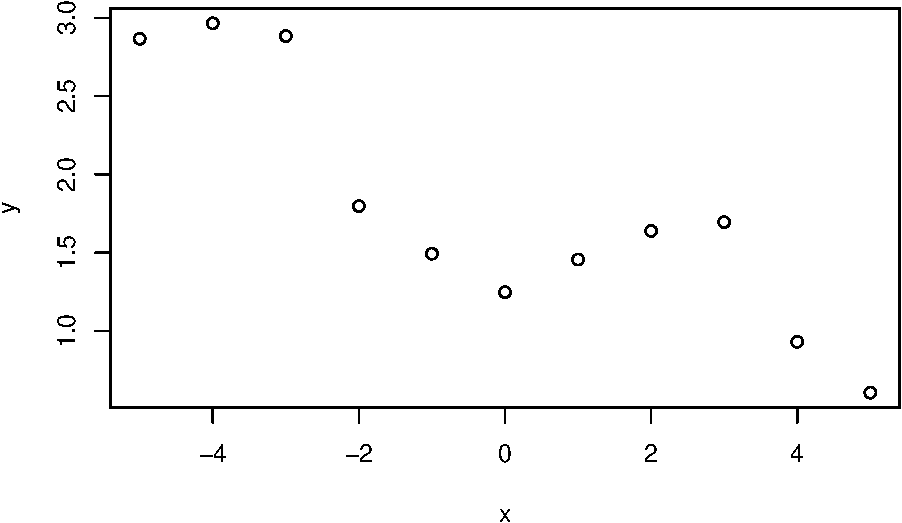
\includegraphics{_main_files/figure-latex/unnamed-chunk-34-1.pdf}

We can see that after about 300 iterations, the Markov chain has converged to its stationary distribution, the posterior distribution. We can see this more clearly by removing the first 300 iterations.

\begin{Shaded}
\begin{Highlighting}[]
\FunctionTok{plot}\NormalTok{(mu.store[}\SpecialCharTok{{-}}\FunctionTok{c}\NormalTok{(}\DecValTok{1}\SpecialCharTok{:}\DecValTok{300}\NormalTok{)], }\AttributeTok{type =} \StringTok{\textquotesingle{}l\textquotesingle{}}\NormalTok{, }\AttributeTok{xlab =} \StringTok{"iteration"}\NormalTok{, }\AttributeTok{ylab =} \FunctionTok{expression}\NormalTok{(mu))}
\end{Highlighting}
\end{Shaded}

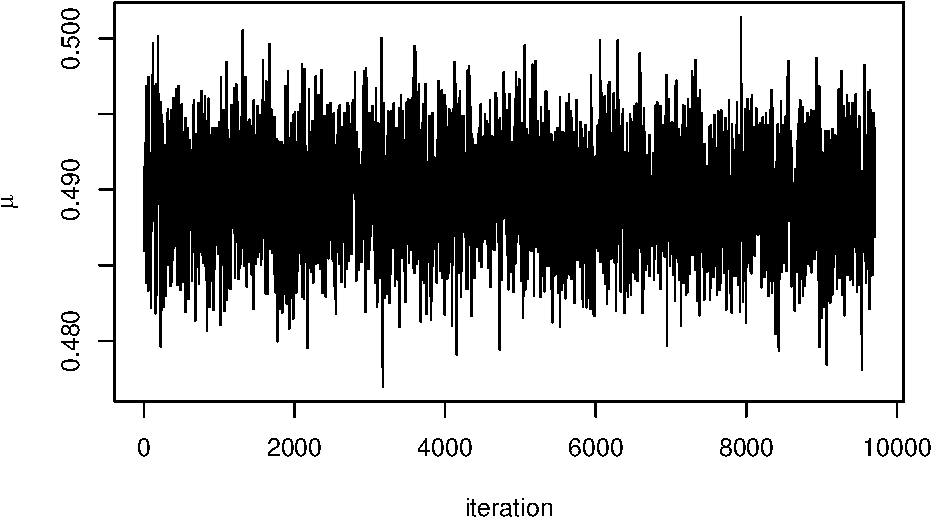
\includegraphics{_main_files/figure-latex/unnamed-chunk-35-1.pdf}

\begin{Shaded}
\begin{Highlighting}[]
\FunctionTok{hist}\NormalTok{(mu.store[}\SpecialCharTok{{-}}\FunctionTok{c}\NormalTok{(}\DecValTok{1}\SpecialCharTok{:}\DecValTok{300}\NormalTok{)], }\AttributeTok{xlab =} \FunctionTok{expression}\NormalTok{(mu), }\AttributeTok{main =} \StringTok{"Posterior distribution"}\NormalTok{)}
\end{Highlighting}
\end{Shaded}

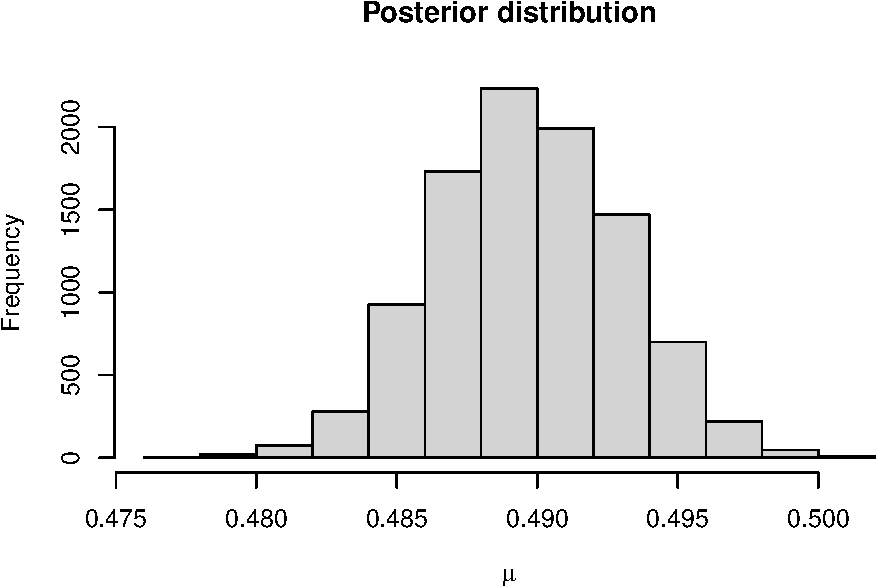
\includegraphics{_main_files/figure-latex/unnamed-chunk-35-2.pdf}

The 95\% credible interval for \(\mu\) using this prior distribution is

\begin{Shaded}
\begin{Highlighting}[]
\FunctionTok{quantile}\NormalTok{(mu.store[}\SpecialCharTok{{-}}\FunctionTok{c}\NormalTok{(}\DecValTok{1}\SpecialCharTok{:}\DecValTok{300}\NormalTok{)], }\FunctionTok{c}\NormalTok{(}\FloatTok{0.025}\NormalTok{, }\FloatTok{0.975}\NormalTok{))}
\end{Highlighting}
\end{Shaded}

\begin{verbatim}
##      2.5%     97.5% 
## 0.4832146 0.4961484
\end{verbatim}

Using a normal prior distribution, it was

\begin{verbatim}
0.486 0.493
\end{verbatim}

It seems that the posterior distribution is very similar when using these two prior distributions. This is because the data are very informative.
\end{example}

\begin{example}
In Lab 3.9, we computed the MAP estimate for a parameter from the Pareto distribution. The density function of this distribution is
\[
\pi(x \mid \beta) = \frac{\beta}{x^{\beta + 1}}, \quad x > 1. 
\]
Placing a Gamma prior distribution on \(\beta\) such that \(\beta \sim \Gamma(a, b)\). The posterior distribution given the data \(\boldsymbol{y} = \{y_1, \ldots, y_N\}\) is
\[
\pi(\beta \mid \boldsymbol{y}) \propto \frac{\beta^{N + a - 1}e^{-b\beta}}{\prod y_i^{\beta + 1}}.
\]
We can't sample from this directly, so wee need to use a Metropolis-Hastings algorithm to generate samples from the posterior distribution. We will use a normal proposal distribution.

The acceptance probability is
\[
p_{acc} = \min \left\{1, \frac{\beta'^{N + a - 1}e^{-b\beta'}}{\prod y_i^{\beta' + 1}}\frac{\prod y_i^{\beta + 1}}{\beta^{N + a - 1}e^{-b\beta}} \right\} \\
= \min \left\{1, \left(\frac{\beta'}{\beta}\right)^{N + a - 1}{\prod y_i^{\beta - \beta'}}\exp((\beta - \beta')b) \right\}. 
\]
The MCMC algorithm will be

\begin{enumerate}
\def\labelenumi{\arabic{enumi}.}
\tightlist
\item
  Set an initial value for \(\beta_1\) and set \(i =1\).
\item
  Propose a new value \(\beta' \sim N(\beta_i, \sigma^2)\)
\item
  Accept \(\beta'\) with probability \(p_{acc}\) and set \(\beta{i+1}= \beta'\), otherwise reject and set\(\beta{i+1}= \beta_i\).
\item
  Repeat steps 2, 3, and 4 for \$ i = 2, \ldots, M\$.
\end{enumerate}

We fix \(b=0.01\) and use the data

\begin{verbatim}
x <- c(1.019844, 1.043574, 1.360953, 1.049228, 1.491926, 1.192943, 1.323738, 1.262572, 2.034768, 1.451654)
\end{verbatim}

to code up our algorithm.

\begin{Shaded}
\begin{Highlighting}[]
\CommentTok{\#Function that evaluates Pareto loglikelihood}
\NormalTok{log.likelihood }\OtherTok{\textless{}{-}} \ControlFlowTok{function}\NormalTok{(x, beta)\{}

\NormalTok{  log.value }\OtherTok{\textless{}{-}} \FunctionTok{length}\NormalTok{(x)}\SpecialCharTok{*}\FunctionTok{log}\NormalTok{(beta) }\SpecialCharTok{{-}}\NormalTok{ (beta }\SpecialCharTok{+} \DecValTok{1}\NormalTok{)}\SpecialCharTok{*}\FunctionTok{sum}\NormalTok{(}\FunctionTok{log}\NormalTok{(x))}

  \FunctionTok{return}\NormalTok{(log.value)}

\NormalTok{\}}

\CommentTok{\# MCMC Sampler {-}{-}{-}{-}{-}{-}{-}{-}{-}{-}{-}{-}{-}{-}{-}{-}{-}{-}{-}{-}{-}{-}{-}{-}{-}{-}{-}{-}{-}{-}{-}{-}{-}{-}{-}{-}{-}{-}{-}{-}{-}{-}{-}{-}{-}{-}{-}{-}{-}{-}{-}{-}{-}{-}{-}{-}{-}{-}{-}{-}}

\CommentTok{\#Initialise Values}
\NormalTok{x }\OtherTok{\textless{}{-}} \FunctionTok{c}\NormalTok{(}\FloatTok{1.019844}\NormalTok{, }\FloatTok{1.043574}\NormalTok{, }\FloatTok{1.360953}\NormalTok{, }\FloatTok{1.049228}\NormalTok{, }\FloatTok{1.491926}\NormalTok{, }\FloatTok{1.192943}\NormalTok{, }\FloatTok{1.323738}\NormalTok{, }\FloatTok{1.262572}\NormalTok{, }\FloatTok{2.034768}\NormalTok{, }\FloatTok{1.451654}\NormalTok{)}
\NormalTok{n.iter }\OtherTok{\textless{}{-}} \DecValTok{10000} \CommentTok{\#number of iterations}
\NormalTok{beta.current }\OtherTok{\textless{}{-}} \DecValTok{2} \CommentTok{\#initial value for beta}
\NormalTok{beta.store }\OtherTok{\textless{}{-}} \FunctionTok{numeric}\NormalTok{(n.iter) }\CommentTok{\#empty vecotr to store beta at each iteration}

\CommentTok{\#Run MCMC For Loop}
\ControlFlowTok{for}\NormalTok{(i }\ControlFlowTok{in} \DecValTok{1}\SpecialCharTok{:}\NormalTok{n.iter)\{}

  \CommentTok{\#Propose prop value for beta}
\NormalTok{  beta.prop }\OtherTok{\textless{}{-}} \FunctionTok{rnorm}\NormalTok{(}\DecValTok{1}\NormalTok{, beta.current, }\FloatTok{0.5}\NormalTok{)}

  \CommentTok{\#Compute current and prop loglikelihood}
\NormalTok{  loglike.prop     }\OtherTok{\textless{}{-}} \FunctionTok{log.likelihood}\NormalTok{(x, beta.prop)}
\NormalTok{  loglike.current }\OtherTok{\textless{}{-}} \FunctionTok{log.likelihood}\NormalTok{(x, beta.current)}

  \CommentTok{\#Compute Log acceptance probability}
\NormalTok{  log.p.acc }\OtherTok{\textless{}{-}}\NormalTok{ loglike.prop }\SpecialCharTok{{-}}\NormalTok{ loglike.current }\SpecialCharTok{+}
    \FunctionTok{dgamma}\NormalTok{(beta.prop, }\DecValTok{1}\NormalTok{, }\FloatTok{0.01}\NormalTok{, }\AttributeTok{log =} \ConstantTok{TRUE}\NormalTok{) }\SpecialCharTok{{-}} \FunctionTok{dgamma}\NormalTok{(beta.current, }\DecValTok{1}\NormalTok{, }\FloatTok{0.01}\NormalTok{, }\AttributeTok{log =} \ConstantTok{TRUE}\NormalTok{)}

  \CommentTok{\#Accept/Reject}
\NormalTok{  u }\OtherTok{\textless{}{-}} \FunctionTok{runif}\NormalTok{(}\DecValTok{1}\NormalTok{)}
  \ControlFlowTok{if}\NormalTok{(}\FunctionTok{log}\NormalTok{(u) }\SpecialCharTok{\textless{}}\NormalTok{ log.p.acc)\{}
\NormalTok{    beta.current }\OtherTok{\textless{}{-}}\NormalTok{ beta.prop}
\NormalTok{  \}}

  \CommentTok{\#Store Current Value}
\NormalTok{  beta.store[i] }\OtherTok{\textless{}{-}}\NormalTok{ beta.current}


\NormalTok{\}}

\CommentTok{\#Plot trace plots}
\FunctionTok{plot}\NormalTok{(beta.store, }\AttributeTok{type =} \StringTok{\textquotesingle{}l\textquotesingle{}}\NormalTok{)}
\end{Highlighting}
\end{Shaded}

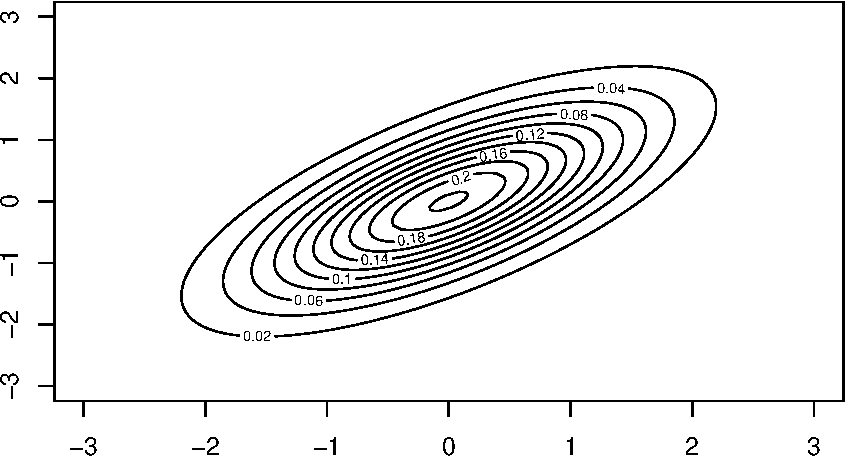
\includegraphics{_main_files/figure-latex/unnamed-chunk-37-1.pdf}

\begin{Shaded}
\begin{Highlighting}[]
\CommentTok{\#Investigate posterior}
\FunctionTok{hist}\NormalTok{(beta.store, }\AttributeTok{freq =} \ConstantTok{FALSE}\NormalTok{, }\AttributeTok{main =} \StringTok{""}\NormalTok{, }\AttributeTok{xlab =} \FunctionTok{expression}\NormalTok{(beta))}
\end{Highlighting}
\end{Shaded}

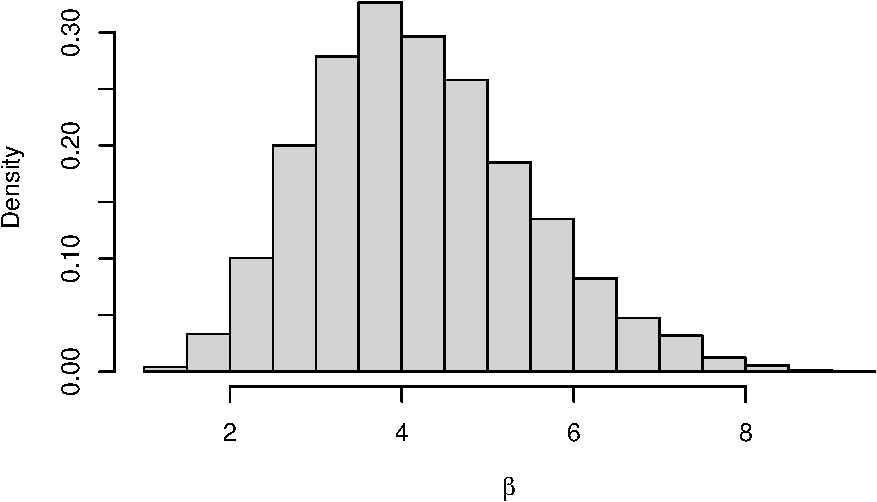
\includegraphics{_main_files/figure-latex/unnamed-chunk-37-2.pdf}

\begin{Shaded}
\begin{Highlighting}[]
\FunctionTok{quantile}\NormalTok{(beta.store, }\FunctionTok{c}\NormalTok{(}\FloatTok{0.025}\NormalTok{, }\FloatTok{0.975}\NormalTok{))}
\end{Highlighting}
\end{Shaded}

\begin{verbatim}
##     2.5%    97.5% 
## 2.102268 7.027826
\end{verbatim}

\hypertarget{gibbs-sampler}{%
\section{Gibbs Sampler}\label{gibbs-sampler}}

When we can sample directly from full conditional distributions, we can use a Gibbs sampler. Suppose we have a distribution with parameters \(\{\theta_1, \ldots, \theta_N\}\), a Gibbs sampler works as follows:

\begin{enumerate}
\def\labelenumi{\arabic{enumi}.}
\item
  Set initial values \(\{\theta_1^{(0)}, \ldots, \theta_N^{(0)}\}\)
\item
  Set \(i = 1\).
\item
  Draw a value for \(\theta_1^{(i)}\) from \(\pi(\theta_1 \mid \theta_2^{(i-1)}, \ldots, \theta_N^{(i-1)}))\).
\item
  Draw a value for \(\theta_2^{(i)}\) from \(\pi(\theta_2 \mid \theta_1^{(i-1)}, \theta_3^{(i-1)}, \ldots, \theta_N^{(i-1)}))\).
\item
  Repeat steps 3 and 4 for parameters \(\{\theta_3^{(i)}, \ldots, \theta_N^{(i)}\}\).
\item
  Repeat steps 3, 4, and 5, for \(i = 2, \ldots M\).
\end{enumerate}

In code, this might look like

\begin{verbatim}
M #number of iterations
N #number of parameters
theta.store   <- matrix(NA, N, M)
theta         <- numeric(N)

for(j in 1:M){
  for(j in 1:N){
    theta[i] <- #sample from conditional with theta[-i]
  }
  theta.store[, j] <- theta.current #store current values
}
\end{verbatim}

\begin{example}
In Example 3.5, we had a hierarchical model with\\
\begin{align*}
\boldsymbol{y} \mid \lambda &\sim \hbox{Exp}(\lambda) & \textrm{(likelihood)} \\
\lambda \mid \gamma &\sim \hbox{Exp}(\gamma) & \textrm{(prior distribution)} \\
\gamma \mid \nu &\sim \hbox{Exp}(\nu) & \textrm{(hyperprior distribution)}  \\
\end{align*}.
To derive the full conditional distributions, we only consider the terms in the posterior distributions that depends on the parameters we are interested in. The full conditional distribution for \(\lambda\) is
\[
\pi(\lambda \mid \boldsymbol{y}, \,\gamma) \propto \lambda^{10}e^{-\lambda(95 + \gamma)}.
\]
This is unchanged and shows that \(\lambda \mid \boldsymbol{y}, \gamma \sim \textrm{Gamma}(11, 95 + \gamma)\). The full conditional distribution for \(\gamma\) is
\[
\pi(\gamma \mid \boldsymbol{y}, \,\lambda) \propto e^{-\nu\gamma}.
\]
Therefore the full conditional distribution of \(\gamma\) is \(\gamma \mid \boldsymbol{y}, \,\lambda \sim \hbox{Exp}(\lambda + \nu)\).

We can set up a Metropolis-Hastings algorithm using Gibbs samplers to generate samples for \(\lambda\) and \(\gamma\).

\begin{enumerate}
\def\labelenumi{\arabic{enumi}.}
\item
  Set initial values \(\{\lambda^{(0)}, \gamma^{(0)}\}\)
\item
  Set \(i = 1\).
\item
  Draw a value for \(\lambda^{(i)} \mid \boldsymbol{y}, \gamma^{(i-1)} \sim \textrm{Gamma}(10, 95 + \gamma^{(i-1)})\)
\item
  Draw a value for \(\gamma^{(i)} \mid \boldsymbol{y}, \,\lambda^{(i)} \sim \hbox{Exp}(\lambda^{(i)} + \nu)\).
\item
  Repeat steps 3 and 4 for \(i = 2, \ldots M\).
\end{enumerate}

We can now code this up and run the algorithm.

\begin{Shaded}
\begin{Highlighting}[]
\CommentTok{\# Set Up MCMC Algorithm {-}{-}{-}{-}{-}{-}{-}{-}{-}{-}{-}{-}{-}{-}{-}{-}{-}{-}{-}{-}{-}{-}{-}{-}{-}{-}{-}{-}{-}{-}{-}{-}{-}{-}{-}{-}{-}{-}{-}{-}{-}{-}{-}{-}{-}{-}{-}{-}{-}{-}{-}}

\NormalTok{n.iter }\OtherTok{\textless{}{-}} \DecValTok{10000}
\NormalTok{lambda.store }\OtherTok{\textless{}{-}} \FunctionTok{numeric}\NormalTok{(n.iter) }\CommentTok{\#Store value of Markov chain at end of every iteration}
\NormalTok{gamma.store }\OtherTok{\textless{}{-}} \FunctionTok{numeric}\NormalTok{(n.iter) }\CommentTok{\#Store value of Markov chain at end of every iteration}



\CommentTok{\# Run MCMC Algorithm {-}{-}{-}{-}{-}{-}{-}{-}{-}{-}{-}{-}{-}{-}{-}{-}{-}{-}{-}{-}{-}{-}{-}{-}{-}{-}{-}{-}{-}{-}{-}{-}{-}{-}{-}{-}{-}{-}{-}{-}{-}{-}{-}{-}{-}{-}{-}{-}{-}{-}{-}{-}{-}{-}}
\ControlFlowTok{for}\NormalTok{(i }\ControlFlowTok{in} \DecValTok{2}\SpecialCharTok{:}\NormalTok{n.iter)\{}
  
  \CommentTok{\#Store current value of Markov Chain}
\NormalTok{  lambda.store[i] }\OtherTok{\textless{}{-}} \FunctionTok{rgamma}\NormalTok{(}\DecValTok{1}\NormalTok{, }\DecValTok{10}\NormalTok{, }\DecValTok{95} \SpecialCharTok{+}\NormalTok{ gamma.store[i}\DecValTok{{-}1}\NormalTok{])}
\NormalTok{  gamma.store[i]  }\OtherTok{\textless{}{-}} \FunctionTok{rexp}\NormalTok{(}\DecValTok{1}\NormalTok{, }\FloatTok{0.01} \SpecialCharTok{+}\NormalTok{ lambda.store[i])}
  
\NormalTok{\}}

\CommentTok{\#Plot trace plot (Markov chain values)}
\FunctionTok{plot}\NormalTok{(lambda.store, }\AttributeTok{type =} \StringTok{\textquotesingle{}l\textquotesingle{}}\NormalTok{, }\AttributeTok{xlab =} \StringTok{"iteration"}\NormalTok{, }\AttributeTok{ylab =} \FunctionTok{expression}\NormalTok{(lambda))}
\end{Highlighting}
\end{Shaded}

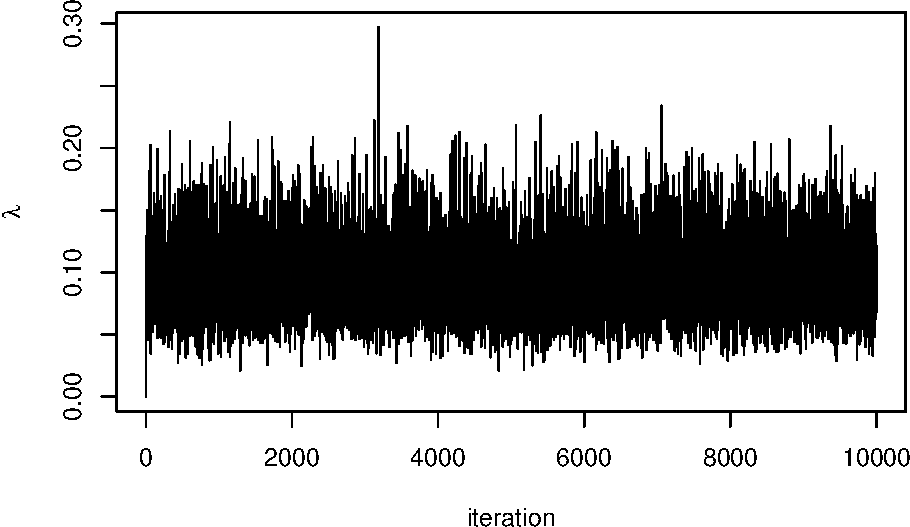
\includegraphics{_main_files/figure-latex/unnamed-chunk-38-1.pdf}

\begin{Shaded}
\begin{Highlighting}[]
\FunctionTok{plot}\NormalTok{(gamma.store, }\AttributeTok{type =} \StringTok{\textquotesingle{}l\textquotesingle{}}\NormalTok{, }\AttributeTok{xlab =} \StringTok{"iteration"}\NormalTok{, }\AttributeTok{ylab =} \FunctionTok{expression}\NormalTok{(gamma))}
\end{Highlighting}
\end{Shaded}

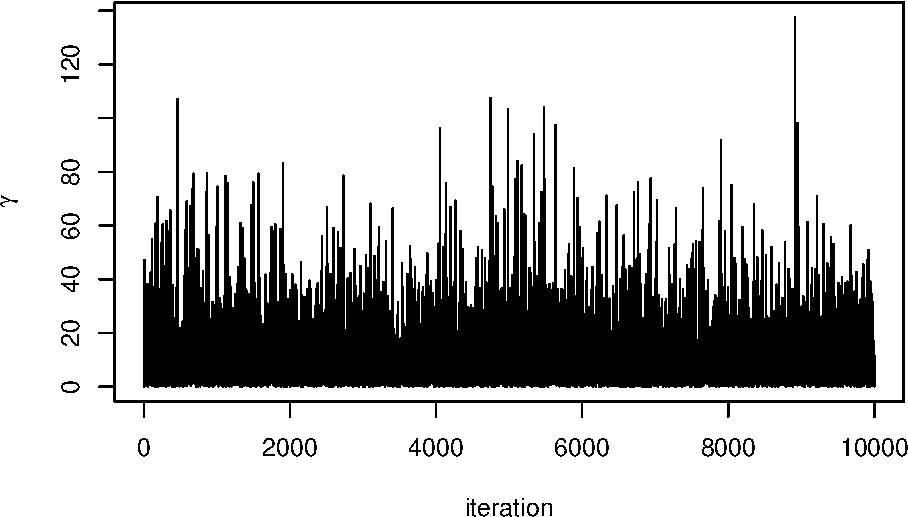
\includegraphics{_main_files/figure-latex/unnamed-chunk-38-2.pdf}

\begin{Shaded}
\begin{Highlighting}[]
\CommentTok{\#Plot posterior density}
\FunctionTok{hist}\NormalTok{(lambda.store, }\AttributeTok{prob =} \ConstantTok{TRUE}\NormalTok{, }\AttributeTok{xlab =} \FunctionTok{expression}\NormalTok{(lambda), }\AttributeTok{main =} \StringTok{"Posterior density"}\NormalTok{)}
\end{Highlighting}
\end{Shaded}

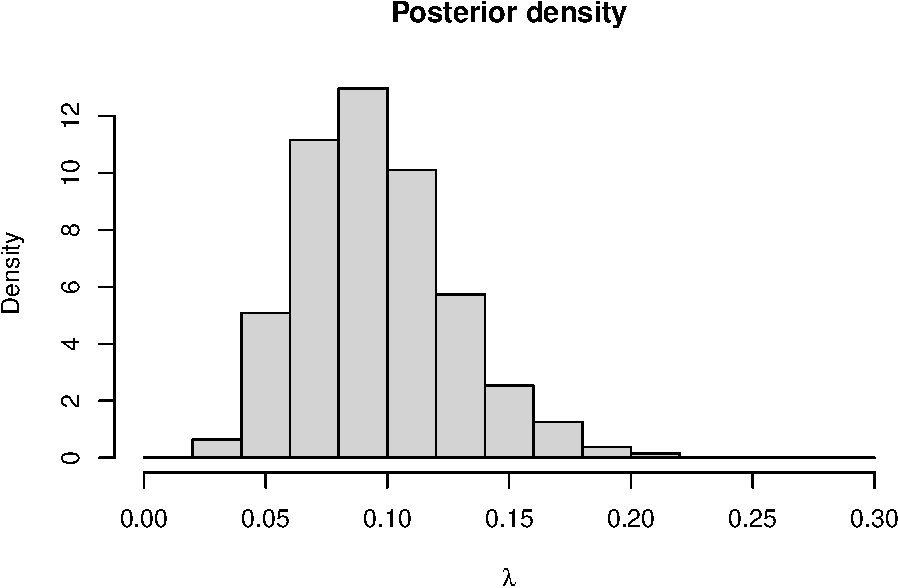
\includegraphics{_main_files/figure-latex/unnamed-chunk-38-3.pdf}

\begin{Shaded}
\begin{Highlighting}[]
\FunctionTok{mean}\NormalTok{(lambda.store) }\CommentTok{\#posterior mean}
\end{Highlighting}
\end{Shaded}

\begin{verbatim}
## [1] 0.09561264
\end{verbatim}

\begin{Shaded}
\begin{Highlighting}[]
\FunctionTok{quantile}\NormalTok{(lambda.store, }\FunctionTok{c}\NormalTok{(}\FloatTok{0.025}\NormalTok{, }\FloatTok{0.975}\NormalTok{)) }\CommentTok{\#95\% CI}
\end{Highlighting}
\end{Shaded}

\begin{verbatim}
##      2.5%     97.5% 
## 0.0454177 0.1658069
\end{verbatim}

\begin{Shaded}
\begin{Highlighting}[]
\FunctionTok{hist}\NormalTok{(gamma.store, }\AttributeTok{prob =} \ConstantTok{TRUE}\NormalTok{, }\AttributeTok{xlab =} \FunctionTok{expression}\NormalTok{(lambda), }\AttributeTok{main =} \StringTok{"Posterior density"}\NormalTok{)}
\end{Highlighting}
\end{Shaded}

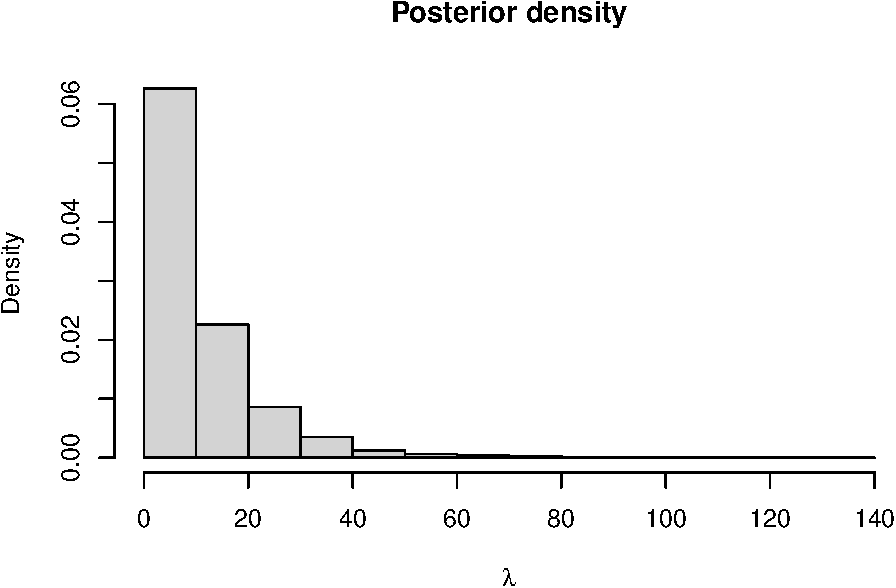
\includegraphics{_main_files/figure-latex/unnamed-chunk-38-4.pdf}

\begin{Shaded}
\begin{Highlighting}[]
\FunctionTok{mean}\NormalTok{(gamma.store) }\CommentTok{\#posterior mean}
\end{Highlighting}
\end{Shaded}

\begin{verbatim}
## [1] 10.4679
\end{verbatim}

\begin{Shaded}
\begin{Highlighting}[]
\FunctionTok{quantile}\NormalTok{(gamma.store, }\FunctionTok{c}\NormalTok{(}\FloatTok{0.025}\NormalTok{, }\FloatTok{0.975}\NormalTok{)) }\CommentTok{\#95\% CI}
\end{Highlighting}
\end{Shaded}

\begin{verbatim}
##       2.5%      97.5% 
##  0.2437085 40.4251992
\end{verbatim}

\begin{Shaded}
\begin{Highlighting}[]
\CommentTok{\#Investogate correlation between parameters}
\FunctionTok{plot}\NormalTok{(lambda.store, gamma.store)}
\end{Highlighting}
\end{Shaded}

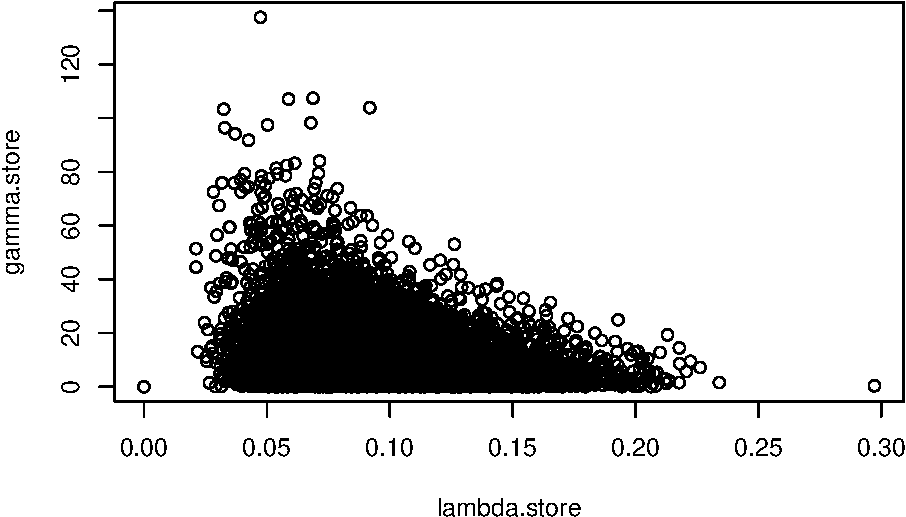
\includegraphics{_main_files/figure-latex/unnamed-chunk-38-5.pdf}
\end{example}

\hypertarget{metropolis-within-gibbs}{%
\section{Metropolis-within-Gibbs}\label{metropolis-within-gibbs}}

Now we have both the Metropolis-Hastings algorithm and Gibbs sampler, we can combine them to create a generic MCMC algorithm for essentially any posterior distribution with any number of parameters. To create our MCMC algorithm, we update any parameters where the full conditional distribution has closed form with a Gibbs sampler. For parameters where the full conditional distribution does not have a closed form, we use a Metropolis-Hastings algorithm to update the parameters.

\begin{example}
Suppose \(X_1, \ldots, X_N \sim \hbox{Weibull}(\beta, \theta)\), where
\[
\pi(x \mid\beta,\theta) = \frac{\beta}{\theta}x^{\beta - 1}\exp\left(-\frac{x^\beta}{\theta}\right), \qquad x, \beta, \theta > 0. 
\]
We use an Exponential prior distribution with rate \(\lambda\) on \(\beta\) and an inverse gamma prior distribution on \(\theta\) such that
\[
\pi(\theta) = \frac{1}{\theta^{a - 1}}\exp\left(-\frac{b}{\theta}\right).
\]
The posterior distribution is therefore
\begin{align*}
\pi(\beta, \theta \mid \boldsymbol{x}) &\propto \pi(\boldsymbol{x} \mid \beta, \theta)\pi(\beta)\pi(\theta) \\
&\propto \frac{\beta^N}{\theta^N}\prod x_i^{\beta - 1}\exp\left(-\frac{1}{\theta}\sum x_i^\beta\right)
\\
&\times\exp(-\lambda\beta) \frac{1}{\theta^{a - 1}}\exp\left(-\frac{b}{\theta}\right)
\end{align*}

The full conditional distributions are therefore
\begin{align*}
\pi(\beta, \mid \theta \boldsymbol{x}) &\propto\beta^N\prod x_i^{\beta - 1}\exp\left(-\frac{1}{\theta}\sum x_i^\beta\right)\exp(-\lambda\beta) \\
\pi(\theta, \mid \beta \boldsymbol{x}) & \frac{1}{\theta^{N + a -1}}\exp\left(-\frac{1}{\theta}(b + \sum x_i^\beta)\right)
\end{align*}

There is no closed form for the full conditional distribution for \(\beta\), so we will need to use a Metropolis-Hastings algorithm to update this parameter in our MCMC algorithm. The full conditional distribution for \(\theta\) is closed as it is proportional to an inverse Gamma distribution with shape \(N + a\) and scale \(b + \sum x_i^\beta\). We can use a Gibbs sampler to update value for \(\theta\). A suitable MCMC algorithm will look like

\begin{enumerate}
\def\labelenumi{\arabic{enumi}.}
\tightlist
\item
  Set initial values for \(\beta^{(0)}\) and \(\theta^{(0)}\) and \(i = 1\).
\item
  Propose a new value for \(\beta\), \(\beta' \sim U[\beta^{(i-1)} + \varepsilon, \beta^{(i-1)} - \varepsilon]\)
\item
  Accept \(\beta' = \beta^{(i)}\) with probability
  \[
  p_{\textrm{acc}} = \min\left\{\frac{\pi(\beta', \theta^{(i-1)} \mid \boldsymbol{x})}{\pi(\beta, \theta^{(i-1)} \mid \boldsymbol{x})}\frac{q(\beta^{(i-1)} \mid \beta')}{q(\beta' \mid \beta^{(i-1)})} , 1\right\}
  \]
  Otherwise reject \(\beta'\) and set \(\beta^{(i)} = \beta^{(i-1)}\).
\item
  Sample \(\theta^{(i)} \sim \hbox{inv}-\Gamma(N + a,\, b + \sum x_i^{\beta^{(i)}})\).
\item
  Repeat steps 2-4.
\end{enumerate}

The acceptance probability in step 3 is the ratio of the full conditional distributions for \(\beta\).
\end{example}

\hypertarget{mcmc-diagnostics}{%
\section{MCMC Diagnostics}\label{mcmc-diagnostics}}

When running an MCMC algorithm, it is always important to check that the Markov chain has converged and is mixing well. For our purposes, mixing well means the chain is exploring the space of possible values of \(\theta\) effectively and effectively and not getting stuck on the same value for a long time.

A key way of doing this is by looking at the trace plot, which is a time series of the posterior samples simulated by the algorithm. The trace plot should look like it has converged to the stationary distribution and exploring the stationary distribution efficiently. What it shouldn't look like is a long series of small steps, or being stuck in one spot for a long time. There are two definitions that help us isolate an efficient Markov chain.

\begin{definition}
The \textbf{burn-in period} is the number of iterations the Markov chain takes to reach the stationary distribution.
\end{definition}

\begin{definition}
The \textbf{thinning parameter} is the period of iterations of the Markov chain that are stored.
\end{definition}

\begin{example}
In Example \ref{exm:norm}, we saw a Markov chain that mixes well. We took the burn-in period to be 3,000 iterations, which was how long it took to for the chain to converge. Although the posterior distribution is invariant to the choice of the proposal distribution, it still has a large effect of the efficiency of the algorithm and how well the chain mixes. The ideal trace plot looks like white noise, or a hairy caterpillar.

In a Metropolis-Hasting random walk algorithm, the proposal distribution often has a large impact on how well the Markov chain mixes. The variance, or step size, of the proposal distribution can be tuned to ensure the chain mixes well.

The following two examples show poorly mixing Markov chains. The first is where the step size is too big and the chain frequently gets stuck for several hundred iterations.

\begin{Shaded}
\begin{Highlighting}[]
\FunctionTok{set.seed}\NormalTok{(}\DecValTok{123}\NormalTok{) }\CommentTok{\#to reproduce}
\NormalTok{n.iter   }\OtherTok{\textless{}{-}} \DecValTok{10000}
\NormalTok{mu.store }\OtherTok{\textless{}{-}} \FunctionTok{numeric}\NormalTok{(n.iter)}

\CommentTok{\#Initial values}
\NormalTok{mu }\OtherTok{\textless{}{-}} \DecValTok{1} 
\NormalTok{sigma }\OtherTok{\textless{}{-}} \FloatTok{0.1} \CommentTok{\#known}

\ControlFlowTok{for}\NormalTok{(i }\ControlFlowTok{in} \DecValTok{1}\SpecialCharTok{:}\NormalTok{n.iter)\{}
  
  \CommentTok{\#Propose value for mu}
\NormalTok{  mu.proposed }\OtherTok{\textless{}{-}} \FunctionTok{runif}\NormalTok{(}\DecValTok{1}\NormalTok{, mu }\SpecialCharTok{{-}} \FloatTok{0.1}\NormalTok{, mu }\SpecialCharTok{+} \FloatTok{0.1}\NormalTok{) }\CommentTok{\#Step size too big}
  
  \ControlFlowTok{if}\NormalTok{(mu.proposed }\SpecialCharTok{\textgreater{}} \DecValTok{0}\NormalTok{)\{ }\CommentTok{\#If mu \textless{} 0 we can reject straight away}
    
    \CommentTok{\#Compute (log) acceptance probability}
\NormalTok{    log.numerator   }\OtherTok{\textless{}{-}} \SpecialCharTok{{-}}\FloatTok{0.01}\SpecialCharTok{*}\NormalTok{mu.proposed }\SpecialCharTok{{-}} 
                        \FunctionTok{sum}\NormalTok{(y }\SpecialCharTok{{-}}\NormalTok{ mu.proposed)}\SpecialCharTok{\^{}}\DecValTok{2}\SpecialCharTok{/}\NormalTok{(}\DecValTok{2}\SpecialCharTok{*}\NormalTok{sigma}\SpecialCharTok{\^{}}\DecValTok{2}\NormalTok{)}
\NormalTok{    log.denominator }\OtherTok{\textless{}{-}} \SpecialCharTok{{-}}\FloatTok{0.01}\SpecialCharTok{*}\NormalTok{mu }\SpecialCharTok{{-}} \FunctionTok{sum}\NormalTok{(y }\SpecialCharTok{{-}}\NormalTok{ mu)}\SpecialCharTok{\^{}}\DecValTok{2}\SpecialCharTok{/}\NormalTok{(}\DecValTok{2}\SpecialCharTok{*}\NormalTok{sigma}\SpecialCharTok{\^{}}\DecValTok{2}\NormalTok{)}
    
\NormalTok{    log.p.acc }\OtherTok{\textless{}{-}}\NormalTok{ log.numerator }\SpecialCharTok{{-}}\NormalTok{ log.denominator}
\NormalTok{    u }\OtherTok{\textless{}{-}} \FunctionTok{runif}\NormalTok{(}\DecValTok{1}\NormalTok{)}
    
    \CommentTok{\#Accept/Reject step}
    \ControlFlowTok{if}\NormalTok{(}\FunctionTok{log}\NormalTok{(u) }\SpecialCharTok{\textless{}}\NormalTok{ log.p.acc)\{}
\NormalTok{      mu }\OtherTok{\textless{}{-}}\NormalTok{ mu.proposed}
\NormalTok{    \}}
\NormalTok{  \}}
  
  \CommentTok{\#Store mu at each iteration}
\NormalTok{  mu.store[i] }\OtherTok{\textless{}{-}}\NormalTok{ mu}
\NormalTok{\}}
\FunctionTok{plot}\NormalTok{(mu.store[}\SpecialCharTok{{-}}\FunctionTok{c}\NormalTok{(}\DecValTok{1}\SpecialCharTok{:}\DecValTok{3000}\NormalTok{)], }\AttributeTok{type =} \StringTok{\textquotesingle{}l\textquotesingle{}}\NormalTok{, }\AttributeTok{xlab =} \StringTok{"iteration"}\NormalTok{, }
     \AttributeTok{ylab =} \FunctionTok{expression}\NormalTok{(mu))}
\end{Highlighting}
\end{Shaded}

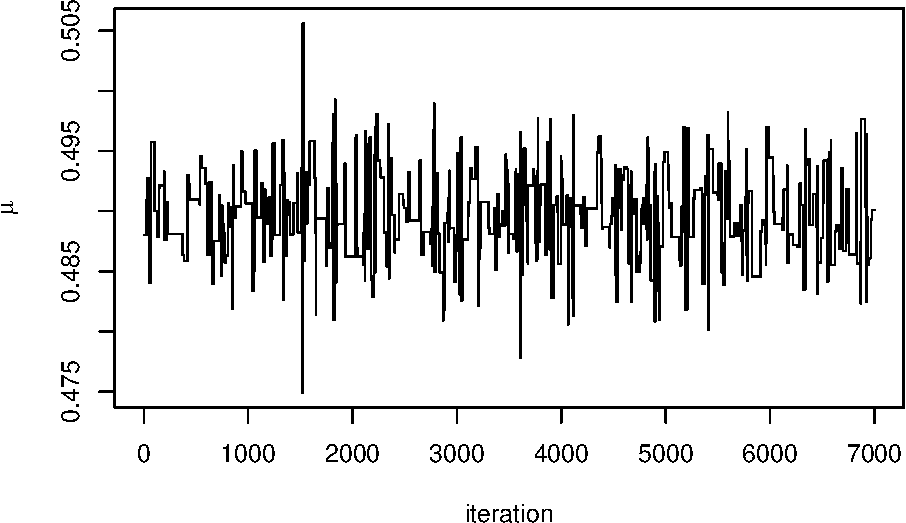
\includegraphics{_main_files/figure-latex/unnamed-chunk-39-1.pdf}

The next is where the step size is too small. It takes a long time for the chain to converge (\textasciitilde50\% of the run time). When the chain does converge, it is inefficient at exploring the space.

\begin{Shaded}
\begin{Highlighting}[]
\FunctionTok{set.seed}\NormalTok{(}\DecValTok{123}\NormalTok{) }\CommentTok{\#to reproduce}
\NormalTok{n.iter   }\OtherTok{\textless{}{-}} \DecValTok{10000}
\NormalTok{mu.store }\OtherTok{\textless{}{-}} \FunctionTok{numeric}\NormalTok{(n.iter)}

\CommentTok{\#Initial values}
\NormalTok{mu }\OtherTok{\textless{}{-}} \DecValTok{1} 
\NormalTok{sigma }\OtherTok{\textless{}{-}} \FloatTok{0.1} \CommentTok{\#known}

\ControlFlowTok{for}\NormalTok{(i }\ControlFlowTok{in} \DecValTok{1}\SpecialCharTok{:}\NormalTok{n.iter)\{}
  
  \CommentTok{\#Propose value for mu}
\NormalTok{  mu.proposed }\OtherTok{\textless{}{-}} \FunctionTok{runif}\NormalTok{(}\DecValTok{1}\NormalTok{, mu }\SpecialCharTok{{-}} \FloatTok{0.0005}\NormalTok{, mu }\SpecialCharTok{+} \FloatTok{0.0005}\NormalTok{) }\CommentTok{\#Step size too small}
  
  \ControlFlowTok{if}\NormalTok{(mu.proposed }\SpecialCharTok{\textgreater{}} \DecValTok{0}\NormalTok{)\{ }\CommentTok{\#If mu \textless{} 0 we can reject straight away}
    
    \CommentTok{\#Compute (log) acceptance probability}
\NormalTok{    log.numerator   }\OtherTok{\textless{}{-}} \SpecialCharTok{{-}}\FloatTok{0.01}\SpecialCharTok{*}\NormalTok{mu.proposed }\SpecialCharTok{{-}}
                        \FunctionTok{sum}\NormalTok{(y }\SpecialCharTok{{-}}\NormalTok{ mu.proposed)}\SpecialCharTok{\^{}}\DecValTok{2}\SpecialCharTok{/}\NormalTok{(}\DecValTok{2}\SpecialCharTok{*}\NormalTok{sigma}\SpecialCharTok{\^{}}\DecValTok{2}\NormalTok{)}
\NormalTok{    log.denominator }\OtherTok{\textless{}{-}} \SpecialCharTok{{-}}\FloatTok{0.01}\SpecialCharTok{*}\NormalTok{mu }\SpecialCharTok{{-}} \FunctionTok{sum}\NormalTok{(y }\SpecialCharTok{{-}}\NormalTok{ mu)}\SpecialCharTok{\^{}}\DecValTok{2}\SpecialCharTok{/}\NormalTok{(}\DecValTok{2}\SpecialCharTok{*}\NormalTok{sigma}\SpecialCharTok{\^{}}\DecValTok{2}\NormalTok{)}
    
\NormalTok{    log.p.acc }\OtherTok{\textless{}{-}}\NormalTok{ log.numerator }\SpecialCharTok{{-}}\NormalTok{ log.denominator}
\NormalTok{    u }\OtherTok{\textless{}{-}} \FunctionTok{runif}\NormalTok{(}\DecValTok{1}\NormalTok{)}
    
    \CommentTok{\#Accept/Reject step}
    \ControlFlowTok{if}\NormalTok{(}\FunctionTok{log}\NormalTok{(u) }\SpecialCharTok{\textless{}}\NormalTok{ log.p.acc)\{}
\NormalTok{      mu }\OtherTok{\textless{}{-}}\NormalTok{ mu.proposed}
\NormalTok{    \}}
\NormalTok{  \}}
  
  \CommentTok{\#Store mu at each iteration}
\NormalTok{  mu.store[i] }\OtherTok{\textless{}{-}}\NormalTok{ mu}
\NormalTok{\}}
\FunctionTok{par}\NormalTok{(}\AttributeTok{mfrow =} \FunctionTok{c}\NormalTok{(}\DecValTok{1}\NormalTok{, }\DecValTok{2}\NormalTok{))}
\FunctionTok{plot}\NormalTok{(mu.store, }\AttributeTok{type =} \StringTok{\textquotesingle{}l\textquotesingle{}}\NormalTok{, }\AttributeTok{xlab =} \StringTok{"iteration"}\NormalTok{, }\AttributeTok{ylab =} \FunctionTok{expression}\NormalTok{(mu))}
\FunctionTok{plot}\NormalTok{(mu.store[}\SpecialCharTok{{-}}\FunctionTok{c}\NormalTok{(}\DecValTok{1}\SpecialCharTok{:}\DecValTok{5000}\NormalTok{)], }\AttributeTok{type =} \StringTok{\textquotesingle{}l\textquotesingle{}}\NormalTok{, }\AttributeTok{xlab =} \StringTok{"iteration"}\NormalTok{,}
     \AttributeTok{ylab =} \FunctionTok{expression}\NormalTok{(mu))}
\end{Highlighting}
\end{Shaded}

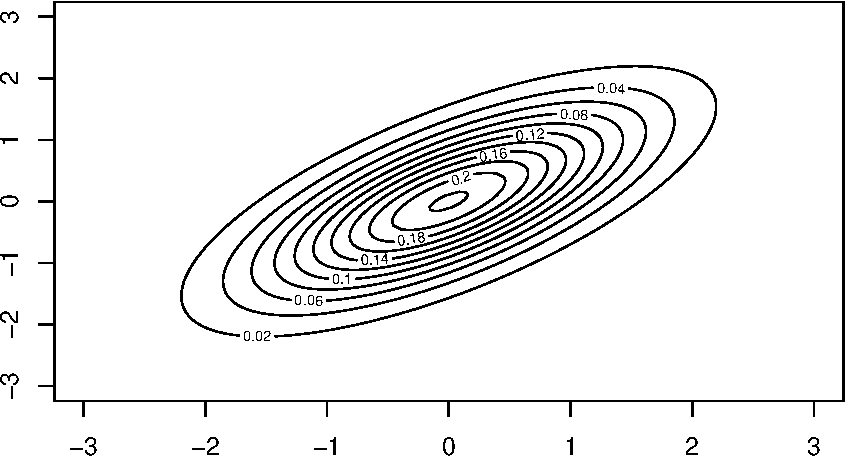
\includegraphics{_main_files/figure-latex/unnamed-chunk-40-1.pdf}
\end{example}

The final diagnostic issue we are going to think about is the \textbf{curse of dimensionality}. In general, the more parameters we try and update, the less likely we are to accept them. This makes exploring the proposal distribution hard if we are trying to update lots of parameters simultaneously. We can see this if we consider a hypersphere
:::\{.example\}
Suppose we have a density function that is uniformly distributed over the area of a sphere in \(N\) dimensions with radius \(r\). The sphere has volume
\[
V = \frac{\pi^{N/2}}{\Gamma(\frac{N}{2} + 1)}r^N.
\]
Now consider a smaller sphere inside of our original sphere. This still has dimension \(N\) but has radius \(r_1 < r\). This small sphere has volume
\[
V_1 = \frac{\pi^{N/2}}{\Gamma(\frac{N}{2} + 1)}r_1^N.
\]
The difference between these two volumes is
\[
V - V_1 = \frac{\pi^{N/2}}{\Gamma(\frac{N}{2} + 1)}(r^N - r_1^N).
\]
For large \(N\), even when \(r - r_1\) is small, \((r^N - r_1^N)\) is large. This means that lots of the probability mass is concentrated away from the mode into the outer shell of the sphere.
\end{example}

The hypersphere example shows that in large dimensions we need our Markov chain to spend lots of time away from the posterior mode and in the tails of the distribution, but this is where the proposal distribution has lowest mass. We can avoid this by updating each parameter individually, but this means we need to use the full conditional distributions, which have highest mass near the mode. This `curse' makes MCMC algorithms inefficient for large dimensions.

\hypertarget{beyond-mcmc}{%
\section{Beyond MCMC}\label{beyond-mcmc}}

MCMC is not the only method available to generate samples from the posterior distribution. MCMC is often slow and inefficient. Much of the work in computational statistics research is about developing fast and efficient methods for sampling from posterior distributions. We are going to look at another method, called approximate Bayesian computation, in the next chapter. Two other methods, beyound the scope of this module, are Sequential Monte Carlo and Hamiltonian Monte Carlo.

Sequential Monte Carlo (SMC) methods for Bayesian inference aim to estimate the posterior distribution of a state space model recursively based on the observed data. Initially, a set of particles representing possible states is sampled from the prior distribution. Then particles are propagated forward using the system dynamics and updated according to their likelihood given the observed data. This update step involves reweighting particles based on how well they explain the observed data. To ensure that the particle set accurately represents the posterior distribution, resampling is performed, where particles with higher weights are more likely to be retained. By iteratively repeating these steps, SMC effectively tracks the evolution of the posterior distribution over time, providing a flexible and computationally efficient framework for Bayesian inference in dynamic systems.

Hamiltonian Monte Carlo (HMC) is a sophisticated Markov chain Monte Carlo (MCMC) method for sampling from complex, high-dimensional target distributions, commonly used in Bayesian inference. Unlike traditional MCMC methods, which rely on random walk proposals, HMC employs Hamiltonian dynamics to guide the exploration of the state space. By introducing auxiliary momentum variables, HMC constructs a joint distribution over the original target variables and the momentum variables. This augmented space enables the use of Hamiltonian dynamics, which can efficiently explore the target distribution by simulating the evolution of the system's energy function. The key idea is to use the gradient of the target distribution's log-probability to determine the momentum dynamics, leading to more effective proposals that can traverse the state space more efficiently. HMC samples are obtained by simulating Hamiltonian dynamics over a trajectory and then accepting or rejecting the proposed states based on Metropolis-Hastings criteria. Overall, HMC offers significant improvements in exploration efficiency compared to traditional MCMC methods, particularly in high-dimensional spaces, making it a powerful tool for Bayesian inference.

\hypertarget{lab-2}{%
\section{Lab}\label{lab-2}}

\begin{exercise}
You observe the following draws from a Binomial distribution with 25 trials and probability of success \(p\).

\begin{verbatim}
y <- c(20, 16, 20, 17, 18, 19, 19, 18, 21, 20, 19, 22, 23, 19, 20, 19, 21, 20, 25, 15)
\end{verbatim}

Use a normal prior distribution with mean 0.5 and variance \(0.1^2\). Write a Metropolis-Hastings Random Walk algorithm to obtain samples from the posterior distribution (you can use R's built in function for the likelihood function and prior distribution, but if you don't take logs you will run into small number errors).
\end{exercise}

\begin{exercise}
In a medical trial, to investigate the proportion \(p\) of the population who have a particular disease a random sample of 20 individuals is taken. Ten of these are subject to a diagnostic test (Test A) which detects the disease when it is present with 100\% certainty. The remaining 10 are given a test (test B) which only detects the disease with probability 0.8 when it is present. Neither test can give a false positive result. before collecting the data your prior belief about \(p\) is represented by a U(0,1) distribution. Suppose that, for Test A, 5 out of 10 test positive while for test B, 3 out of 10 test positive. Use an MCMC algorithm to investigate the posterior density of \(p\) and estimate its posterior mean and variance.
\end{exercise}

\begin{exercise}
Code up an MCMC algorithm for Example 3.5 using Gibbs samplers.
\end{exercise}

\begin{exercise}
The density function for the inverse-gamma distribution is
\[
\pi(x\mid \alpha, \beta) = \frac{\beta^\alpha}{\Gamma(\alpha)}x^{\alpha - 1}e^{-\beta/x}
\]
Using independent Gamma prior distributions on the model parameters, \(\alpha \sim \Gamma(a, b)\) and \(\beta \sim Gamma(c, d)\), write down the posterior distribution for the model parameters. Only one will have a closed form.

Develop a code an MCMC algorithm to sample from the posterior distribution by alternating between sampling \(\alpha\) and then \(\beta\).

Simulate some data from the inverse-gamma distribution and see if you can recover the parameters used to simulate the data. Is there any correlation between the samples for \(\alpha\) and \(\beta\).
\end{exercise}

\hypertarget{advanced-computation}{%
\chapter{Advanced Computation}\label{advanced-computation}}

Now we have the tools of Bayesian inference and methods to sample from complex posterior distributions, we can start to look at more advanced methods and models. This chapter is split into four distinct parts, each showing a different method in Bayesian inference.

\hypertarget{gaussian-processes}{%
\section{Gaussian Processes}\label{gaussian-processes}}

So far in the module, we have considered prior distribution on parameters. These parameters have taken values (mostly real) or real-valued vectors. In this section, we're going to extend this idea further to place prior distributions on functions. That is, we're going to describe a prior distribution that when sampled gives us functions. The method we're going to use is called a Gaussian Process (GP).

Before, we define a GP, we're going to build an intuitive definition of it. Recall the normal distribution with mean \(\mu\) and variance \(\sigma^2\), \(N(\mu, \sigma^2)\). It assigns probabilities to values on the real line -- when we sample from it, we get real values. The plot below shows the density function for a \(N(0, 1)\) distribution and five samples.

\begin{Shaded}
\begin{Highlighting}[]
\CommentTok{\#Plot N(0, 1)}
\NormalTok{x }\OtherTok{\textless{}{-}} \FunctionTok{seq}\NormalTok{(}\SpecialCharTok{{-}}\DecValTok{4}\NormalTok{, }\DecValTok{4}\NormalTok{, }\FloatTok{0.01}\NormalTok{)}
\NormalTok{y }\OtherTok{\textless{}{-}} \FunctionTok{dnorm}\NormalTok{(x)}
\FunctionTok{plot}\NormalTok{(x, y, }\AttributeTok{type =} \StringTok{\textquotesingle{}l\textquotesingle{}}\NormalTok{)}

\CommentTok{\#Add samples}
\NormalTok{samples }\OtherTok{\textless{}{-}} \FunctionTok{rnorm}\NormalTok{(}\DecValTok{5}\NormalTok{)}
\FunctionTok{rug}\NormalTok{(samples)}
\end{Highlighting}
\end{Shaded}

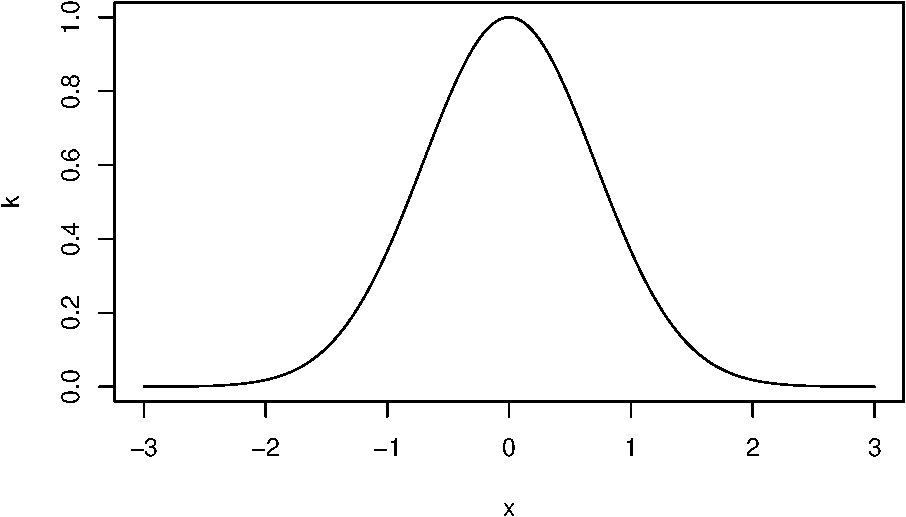
\includegraphics{_main_files/figure-latex/unnamed-chunk-41-1.pdf}

The multivariate normal distribution extends this to a vector space, \(\mathbb{R}^N\). Instead of having a mean and variance value, the distribution is defined through a mean vector and covariance matrix. The mean vector describes the expected value of each component of the vector and the covariance matrix describes the relationship between each pair of components in the vector. When we draw samples, we get vectors. The plot below shows the density of the multivariate normal distribution with \(N = 2\), zero mean, \(\sigma^2_x = \sigma^2_y = 1\) and \(\rho = 0.7\).

\begin{Shaded}
\begin{Highlighting}[]
\CommentTok{\#Create Grid}
\NormalTok{x }\OtherTok{\textless{}{-}} \FunctionTok{seq}\NormalTok{(}\SpecialCharTok{{-}}\DecValTok{3}\NormalTok{,}\DecValTok{3}\NormalTok{,}\AttributeTok{length.out=}\DecValTok{100}\NormalTok{)}
\NormalTok{y }\OtherTok{\textless{}{-}} \FunctionTok{seq}\NormalTok{(}\SpecialCharTok{{-}}\DecValTok{3}\NormalTok{,}\DecValTok{3}\NormalTok{,}\AttributeTok{length.out=}\DecValTok{100}\NormalTok{)}

\CommentTok{\#Evaluate density at grid}
\NormalTok{z }\OtherTok{\textless{}{-}} \FunctionTok{matrix}\NormalTok{(}\DecValTok{0}\NormalTok{,}\AttributeTok{nrow=}\DecValTok{100}\NormalTok{,}\AttributeTok{ncol=}\DecValTok{100}\NormalTok{)}
\NormalTok{mu }\OtherTok{\textless{}{-}} \FunctionTok{c}\NormalTok{(}\DecValTok{0}\NormalTok{,}\DecValTok{0}\NormalTok{)}
\NormalTok{sigma }\OtherTok{\textless{}{-}} \FunctionTok{matrix}\NormalTok{(}\FunctionTok{c}\NormalTok{(}\DecValTok{1}\NormalTok{, }\FloatTok{0.7}\NormalTok{, }\FloatTok{0.7}\NormalTok{, }\DecValTok{1}\NormalTok{),}\AttributeTok{nrow=}\DecValTok{2}\NormalTok{)}
\ControlFlowTok{for}\NormalTok{ (i }\ControlFlowTok{in} \DecValTok{1}\SpecialCharTok{:}\DecValTok{100}\NormalTok{) \{}
  \ControlFlowTok{for}\NormalTok{ (j }\ControlFlowTok{in} \DecValTok{1}\SpecialCharTok{:}\DecValTok{100}\NormalTok{) \{}
\NormalTok{    z[i,j] }\OtherTok{\textless{}{-}}\NormalTok{ mvtnorm}\SpecialCharTok{::}\FunctionTok{dmvnorm}\NormalTok{(}\FunctionTok{c}\NormalTok{(x[i],y[j]),}
                      \AttributeTok{mean=}\NormalTok{mu,}\AttributeTok{sigma=}\NormalTok{sigma)}
\NormalTok{  \}}
\NormalTok{\}}

\CommentTok{\#Generate contour plot}
\FunctionTok{contour}\NormalTok{(x, y ,z)}
\end{Highlighting}
\end{Shaded}

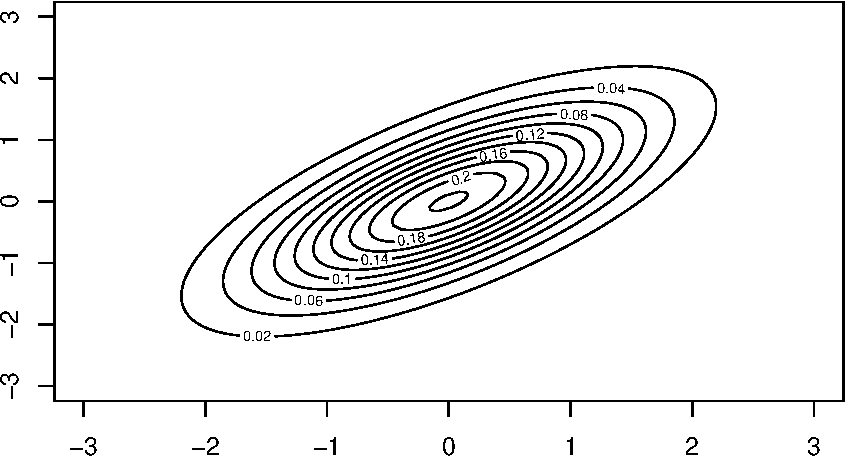
\includegraphics{_main_files/figure-latex/unnamed-chunk-42-1.pdf}

A GP takes this one step further and puts a prior distribution on a function space. It is specified by a mean function, \(\mu(\cdot)\) and covariance function \(k(\cdot, \cdot)\). The mean function describes the expected value of each point the function can be evaluated at, and the covariance function describes the relationship between each point on the function. The plot below shows three samples from a GP distribution with mean function the zero function \(\mu(x) = 0\, \forall x\) and a covariance function that supports smooth functions.

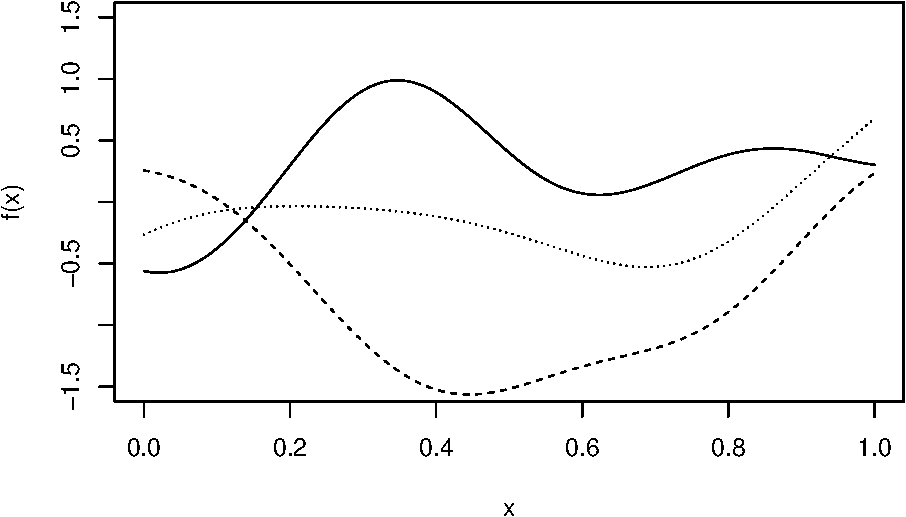
\includegraphics{_main_files/figure-latex/unnamed-chunk-43-1.pdf}

\begin{definition}
A \textbf{Gaussian Process} is a collection of random variables, any finite number of which have a joint Gaussian distribution.
\end{definition}

This says that is we think of a function as an infinite collection of points, then if any finite subset of those points following a Gaussian distribution, we have a Gaussian process. In reality, we set up the function so that is meets this definition. More formally,

\begin{definition}
A \textbf{GP distribution on a function \(f(x)\)} is defined through its mean function \(\mu(x) = \mathbb{E}(x)\) and covariance function \(k(x, x') = \mathbb{E}(x)\left((f(x) - \mu(x))(f(x') - \mu(x'))\right)\). We write it as \(f(x) \sim \mathcal{GP}(\mu(x), k(x, x'))\).
\end{definition}

Before we go any further, it is worth proceeding with caution. Those with good memories will recall Bernstein-von-Mises' theorem from Chapter 3.

\begin{theorem}[Bernstein-von-Mises]
For a well-specified model \(\pi(\boldsymbol{y} \mid \theta)\) with a fixed number of parameters, and for a smooth prior distribution \(\pi(\theta)\) that is non-zero around the MLE \(\hat{\theta}\), then
\[
\left|\left| \pi(\theta \mid \boldsymbol{y}) - N\left(\hat{\theta}, \frac{I(\hat{\theta})^{-1}}{n}\right) \right|\right|_{TV} \rightarrow 0.
\]
\end{theorem}

Bernstein-von-Mises' theorem only holds when the model has a fixed (i.e.~finite) number of parameters. A GP is defined on an infinite collection of points, and so this theorem does not hold. This is the first time in this module we have encountered a distribution where Bernstein-von-Mises' theorem does not hold. Fortunately, various forms of Bernstein-von-Mises' theorems for GPs exist, with many coming about in the early 2010s. However, this is still an ongoing area of research.

\hypertarget{covariance-functions}{%
\subsection{Covariance Functions}\label{covariance-functions}}

One issue when using GPs is describing the covariance function. How do we decide how each pair of points (there being an infinite number of them)? There are lots of standard choices of covariance functions that we can choose from, each one making different assumptions about the function we are interested in.

The most common covariance function is the squared exponential functions. It is used to model functions that are `nice', i.e.~they are smooth, continuous and infinitely differentiable.

\begin{definition}
The \textbf{squared exponential covariance function} takes the form
\[
k(x, x') = \alpha^2\exp\left\{-\frac{1}{l}(x-x')^2\right\},
\]
where \(\alpha^2\) is the signal variance and \(l>0\) is the length scale parameter.
\end{definition}

For now, consider \(\alpha = l = 1\). What is the covariance between the function evaluated at 0 and the function evaluated at \(x\)? The plot below shows the covariance.

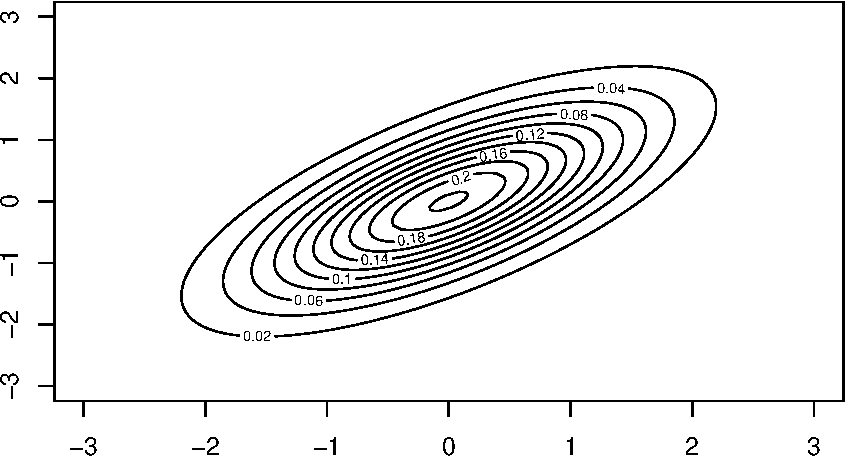
\includegraphics{_main_files/figure-latex/unnamed-chunk-44-1.pdf}

The covariance is highest when the \(x\) is near to 0, i.e.~the points are immediately next to each other. If the value of \(x\) is \(\pm 2\), the covariance is 0. As we are dealing with a joint normal distribution, a covariance of 0 implies independence. So with this covariance function, the value of \(f(x)\) is independent of \(f(0)\) if \(|x|\) is larger than about two. The parameter \(l\) is called the length scale parameter and dictates how quickly the covariance decays. Small values of \(l\) mean that the value of the function at nearby points are independent of each other, resulting in functions that look like white noise. Large values of \(l\) mean that even if points are far away, they are still highly dependent on each other. This gives very flat functions.

The choice of covariance function is a modelling choice -- it depends completely on the data generating process you are trying to model. The following properties are useful when deciding which covariance function to use.

\begin{definition}
A \textbf{stationary} covariance function is a function of \(\boldsymbol{x} - \boldsymbol{x}'\). That means it is invariant to translations in space.
\end{definition}

\begin{definition}
An \textbf{isotropic} covariance function is a function only of \(|\boldsymbol{x} - \boldsymbol{x}'|\). That means it is invariant to rigid translations in space.
\end{definition}

\begin{definition}
An \textbf{dot product} covariance function is a function only of \(\boldsymbol{x}\cdot\boldsymbol{x}'\). That means it is invariant to rigid rotations in space, but not translations.
\end{definition}

What is most important is that the matrix resulting from a covariance function is positive semi-definite. This is because covariance matrices must be positive semi-definite.

\begin{definition}
An \(N \times N\) matrix \(\Sigma\) is positive semi-definite if it is symmetric and
\[
\boldsymbol{x}^T\Sigma\boldsymbol{x} \geq 0 \quad \hbox{for all } \boldsymbol{x} \in \mathbb{R}^N.
\]
\end{definition}

The squared exponential covariance function is isotropic and produces functions that are continuous and differentiable. There are many other types of covariance functions, including ones that don't produce functions that are continuous or differentiable. Three4 more are given below.

\begin{definition}
The \textbf{M\textquotesingle atern} covariance function models functions that are differentiable only once:
\[
k(x, x') = \left(1 + \frac{\sqrt{3}(x - x')^2}{l} \right)\exp\left\{-\frac{\sqrt{3}(x - x')^2}{l} \right\}.
\]
\end{definition}

\begin{definition}
The \textbf{periodic} covariance function models functions that are periodic and it is given by
\[
k(x, x') = \alpha^2 \exp\left\{-\frac{2}{l}\sin^2\frac{(x-x')^2}{p} \right\},
\]
where the period is \(p\).
\end{definition}

\begin{definition}
The \textbf{dot product} covariance function models functions that are rotationally invariant and it is given by
\[
k(x, x') = \alpha^2 + x\cdot x'.
\]
\end{definition}

These are just some covariance functions. In addition to the covariance functions defined, we can make new covariance funcitons by combining existing ones.

\begin{proposition}
If \(k_1\) and \(k_2\) are covariance functions, then so is \(k_1 + k_2\).
\end{proposition}

\begin{proof}
Let \(f_1\) be a function with covariance function \(k_1\) and \(f_2\) be a function with covariance function \(k_2\), then \(f = f_1 + f_2\) has covariance function \(k_1 + k_2\).
\end{proof}

\begin{proposition}
If \(k_1\) and \(k_2\) are covariance functions, then so is \(k_1k_2\).
\end{proposition}

\begin{proof}
See problem sheet.
\end{proof}

\hypertarget{gaussian-process-regression}{%
\subsection{Gaussian Process Regression}\label{gaussian-process-regression}}

One of the main applications of GPs in in regression. Suppose we observe the points below \(\boldsymbol{y} = \{y_1, \ldots, y_N\}\) and want to fit a curve through them. One method is to write down a set of functions of the form \(\boldsymbol{y} = X^T\boldsymbol{\beta} + \boldsymbol{\varepsilon}\), where \(X\) is the design matrix and \(\boldsymbol{\beta}\) a vector of parameters. For each design matrix \(X\), construct the posterior distributions for \(\boldsymbol{\beta}\) and use some goodness-of-fit measure to choose the most suitable design matrix.

\begin{Shaded}
\begin{Highlighting}[]
\NormalTok{x }\OtherTok{\textless{}{-}} \SpecialCharTok{{-}}\DecValTok{5}\SpecialCharTok{:}\DecValTok{5}
\NormalTok{y }\OtherTok{\textless{}{-}} \FunctionTok{sin}\NormalTok{(x}\SpecialCharTok{/}\DecValTok{2}\NormalTok{)}\SpecialCharTok{\^{}}\DecValTok{2} \SpecialCharTok{+} \FunctionTok{exp}\NormalTok{(}\SpecialCharTok{{-}}\NormalTok{x}\SpecialCharTok{/}\DecValTok{5}\NormalTok{) }\SpecialCharTok{+} \FunctionTok{rnorm}\NormalTok{(}\FunctionTok{length}\NormalTok{(x), }\DecValTok{0}\NormalTok{, }\FloatTok{0.2}\NormalTok{)}
\FunctionTok{plot}\NormalTok{(x, y)}
\end{Highlighting}
\end{Shaded}

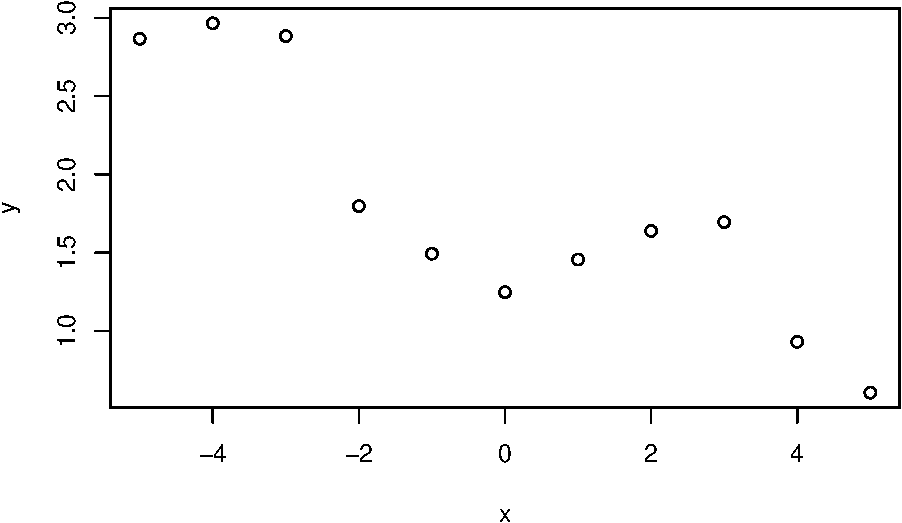
\includegraphics{_main_files/figure-latex/unnamed-chunk-45-1.pdf}

One difficulty is writing down the design matrices \(X\), it is often not straightforward to propose or justify these forms GPs allow us to take a much less arbitrary approach, simply saying that \(y_i = f(x_i) + \varepsilon_i\) and placing a GP prior distribution on \(f\).

Although we're placing an prior distribution with an infinite dimension on \(f\), we only ever need to work with a finite dimensional object, making this much easier. We only observe the function at finite number of points \(\boldsymbol{f} = \{f(x_1), \ldots, f(x_N)\}\) and we will infer the value of the function at points on a fine grid, \(\boldsymbol{f}^* = \{f(x_1^*), \ldots, f(x_N^*)\}\). By the definition of a GP, the distribution of these points is a multivariate normal distribution.

\begin{example}
Suppose we observe \(\boldsymbol{y} = \{y_1, \ldots, y_N\}\) at \(\boldsymbol{x} = \{x_1, \ldots, x_N\}\). The plot below shows these points.

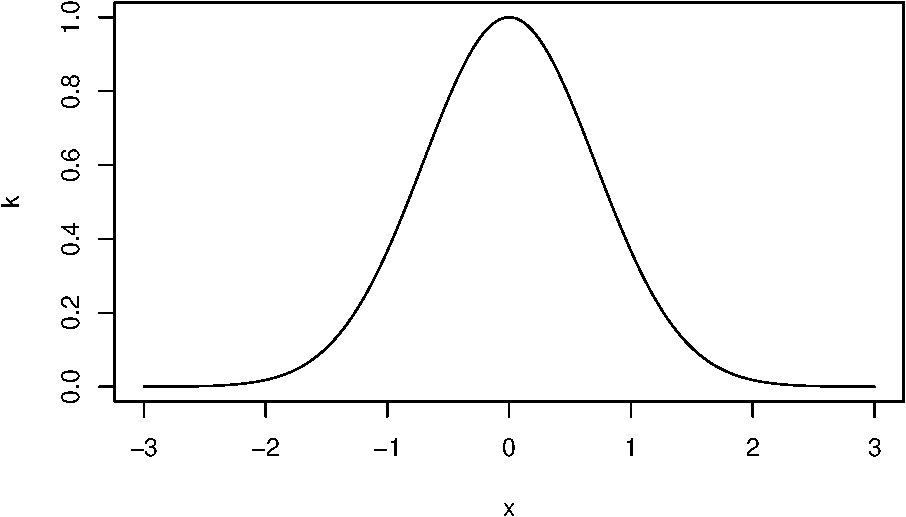
\includegraphics{_main_files/figure-latex/unnamed-chunk-46-1.pdf}

Using the model \(y_i = f(x_i) + \varepsilon_i\), where \(\varepsilon_i \sim N(0, \sigma^2)\), we want to infer the function \(f\) evaluated at a gird of points \(\boldsymbol{f}^* = \{f(x_1^*), \ldots, f(x_N^*)\}\). We place a GP prior distribution on \(f \sim \mathcal{GP}(0, k)\), where \(k\) is the squared exponential covariance function. Using the model, the covariance between points \(y_i\) and \(y_j\) is
\[
\textrm{cov}(y_i, y_j) = k(x_i, x_j) + \sigma^21_{i=j}.
\]
That is the covariance function evaluated at \(x_i\) and \(x_j\) plus \(\sigma^2\) if \(i = j\). We can write this in matrix form as \(K(\boldsymbol{x}, \boldsymbol{x}) + \sigma^2I\) where \(I\) is the identity matrix. The distribution of \(\boldsymbol{y}\) is therefore \(\boldsymbol{y} \sim N(\boldsymbol{0}, \, K(\boldsymbol{x}, \boldsymbol{x}) + \sigma^2I)\). By definition of the GP, the distribution of the function evaluated at the fine grid is \(\boldsymbol{f}^* \sim N(\boldsymbol{0}, K(\boldsymbol{x}^*, \boldsymbol{x}^*))\).

We can now write the joint distribution as
\[
\begin{pmatrix}
\boldsymbol{y} \\
\boldsymbol{f}^*
\end{pmatrix} \sim N\left(\boldsymbol{0}, \,
\begin{pmatrix}
 K(\boldsymbol{x}, \boldsymbol{x}) + \sigma^2I &  K(\boldsymbol{x}, \boldsymbol{x}^*)\\
K(\boldsymbol{x}^*, \boldsymbol{x}) & K(\boldsymbol{x}^*, \boldsymbol{x}^*)
\end{pmatrix}.
\right)
\]
The off-diagonal terms in the covariance matrix describe the relationship between the observed points \(\boldsymbol{y}\) and the points of interest \(\boldsymbol{f}^*\). We can now write down the distribution of \(\boldsymbol{f}^*\) given the observed points \(\boldsymbol{y}\) and \(\sigma^2\).
\[
\boldsymbol{f}^* \mid \boldsymbol{y}, \sigma^2 \sim N(\boldsymbol{\mu}^*, \, K^*),
\]
where \(\boldsymbol{\mu}^* = K(\boldsymbol{x}^*, \boldsymbol{x})(K(\boldsymbol{x}, \boldsymbol{x}) + \sigma^2 I)^{-1} \boldsymbol{y}\) and \(K^* = K(\boldsymbol{x}^*, \boldsymbol{x}^*) - K(\boldsymbol{x}^*, \boldsymbol{x})(K(\boldsymbol{x}, \boldsymbol{x}) + \sigma^2I)^{-1}K(\boldsymbol{x}, \boldsymbol{x}^*)\).

We set the fine gird to be \(\boldsymbol{x}^* = \{-5, -4.99, -4.98, \ldots, 5\}\), the GP parameters \(\alpha = l = 1\) and \(\sigma = 0.2\). The posterior mean and 95\% credible interval are shown below.
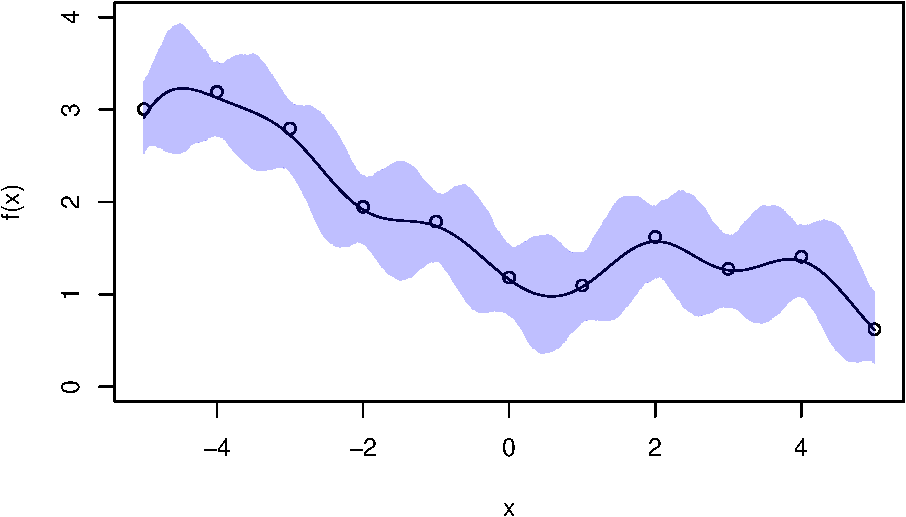
\includegraphics{_main_files/figure-latex/unnamed-chunk-47-1.pdf}
The posterior mean for \(f\) is a smooth line passing near each point. The 95\% credible interval for \(f\) has the smallest variance near each point, and largest furthest away from the points.
\end{example}

\hypertarget{data-augmentation}{%
\section{Data Augmentation}\label{data-augmentation}}

Real world data are often messy with data points missing which may mean they are partially or completely unobserved. One common example of this is in clinical trials where people drop out of the trial before their treatment is complete. Another example is crime data, where only a fraction of crimes are reported and many crimes go unobserved. Two common ways to deal with partially or completely unobserved are:

\begin{itemize}
\tightlist
\item
  Remove data points that are not completely observed. This throws away information and is likely to increase the overall uncertainty in the estimates.
\item
  Replace data points that are not completely observed with estimates such as the sample mean. This is likely to underestimate the uncertainty as we are treating the observation as completely observed when it is not.
\end{itemize}

The Bayesian framework provides a natural way for dealing with missing, partially, or completely unobserved data. It allows us to treat the missing data points as random variables and infer the data points alongside the model parameters. This provides us with a method to quantify the uncertainty around our estimates of the missing data points.

In data augmentation, we distinguish between two likelihood functions.

\begin{definition}
The \textbf{observed data likelihood function} is the likelihood function of the observed data.
\end{definition}

\begin{definition}
The \textbf{complete data likelihood function} is the likelihood function of the observed data and any missing or censored data had they been fully observed.
\end{definition}

The difference between the two likelihood functions is that the complete data likelihood function is the functions had we observed everything we want to observe. However, as the complete data likelihood function contains data we didn't fully observe, we can't compute it. Instead we can only evaluate the observed data likelihood function. A simple probability based example of this is if there are two events \(X\) and \(Y\), where the outcome of \(X\) is observed and \(Y\) unobserved. The complete data likelihood is \(pi(X = x, Y = y)\) because we are considering all the events, observed or not. However, we can only compute \(\pi(x) = \int_{y \in Y}\pi(X = x, Y = y)\) or \(\pi(x) = \sum_{y \in Y}\pi(X = x, Y = y)\), since \(y\) is unobserved.

In data augmentation, we start off with the observed data likelihood function and then augment this function by introducing variables that we want to have fully observed. This then gives us the complete data likelihood function.

\hypertarget{imputing-censored-observations}{%
\subsection{Imputing censored observations}\label{imputing-censored-observations}}

The first example we will look at is when data is censored. Instead of throwing away these observations, we will instead treat them as random variables and infer their values.

\begin{example}
A bank checks transactions for suspicious activities in batches of 1000. Denote the probability a transaction is suspicious by \(p\) and the number of suspicious transactions in a batch by \(Y\).

The bank checks five batches and observes \(y_1, \ldots, y_4\) suspicious transactions in the first four batches. Due to a computer error, the number of suspicious transactions in the final batch is not properly recorded, but is known to be less than 6.

The observed data likelihood functions is
\[
\pi(y_1, \ldots, y_4, \tilde{y}_5 \mid p) = \left(\prod_{i=1}^4\begin{pmatrix} 1000 \\ y_i \end{pmatrix} p^{y_i}(1-p)^{1000 - y_i} \right)\left(\sum_{j=0}^5\begin{pmatrix} 1000 \\ j \end{pmatrix} p^{j}(1-p)^{1000 - j}\right).
\]
This is known as marginalising over the missing variable, just as we did in the simple probability example earlier. Placing a uniform prior distribution on \(p \sim U[0, 1]\) give the posterior distribution
\[
\pi(p \mid y_1, \ldots, y_4, \tilde{y}_5)= \left(\prod_{i=1}^4\begin{pmatrix} 1000 \\ y_i \end{pmatrix} p^{y_i}(1-p)^{y_i} \right)\left(\sum_{j=0}^5\begin{pmatrix} 1000 \\ j \end{pmatrix} p^{j}(1-p)^{1000 - j}\right).
\]
Although we could sample from this distribution, it is not easy to work with. Instead, we can write down the complete data likelihood. Suppose that \(y_5\) was observed, then the complete data likelihood may be written as
\[
\pi(y_1, \ldots, y_5 \mid p)  = \prod_{i=1}^5\begin{pmatrix} 1000 \\ y_i \end{pmatrix} p^{y_i}(1-p)^{1000 - y_i},
\]
The posterior distribution is therefore
\[
p \mid y_1, \ldots, y_5 \sim \hbox{Beta}\left(\sum_{i=1}^5 y_i + 1, 5000 + 1 - \sum_{i=1}^5 y_i\right).
\]

The full conditional distribution of \(y_5\) given \(p\), the other data points an \(y_5 < 6\) is
\[
  \pi(y_5 = y \mid y_1, \ldots, y_4, y_5 < 6, p) = \frac{\begin{pmatrix} 1000 \\ y \end{pmatrix} p^{y}(1-p)^{1000 - y}}{\sum_{j=0}^{5}\begin{pmatrix} 1000 \\ j \end{pmatrix} p^{j}(1-p)^{1000-j}}, \qquad y < 6
\]
We can use a Gibbs sampler alternating between sampling \(p\) and \(y_5\).
\end{example}

\hypertarget{imputing-latent-variables}{%
\subsection{Imputing Latent Variables}\label{imputing-latent-variables}}

Often there are variables that are cannot be observed, these may be hidden somehow or introduced to help with the modelling. Instead we can learn about this variable indirectly from the data.

A \textbf{latent variable} is a variable that cannot be observed.

A mixture model is an example of latent variables being useful.

\begin{example}
Royal Mail use image detection software to read postcodes on letters. A camera scans the front of an envelope and then records the barcode. This example is a very simplified version of how the system could work.

Suppose the machine is processing a bag of letters addressed to people in either B1 or B2 postcodes. The camera scans the first two characters of the postcode (B1 or B2) and records the proportion of the scanned image that is taken up by the characters. The picture below shows an example of what the scanned image looks like.

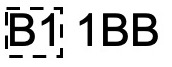
\includegraphics{postcode.jpeg}
The scanned image is a 10 by 10 grid of pixels, where the number of pixels coloured black of the \(i^{th}\) image is \(Y_i \sim \hbox{Bin}(100, \theta)\). However, \(\theta\) depends on if the letter is going to B1 or B2. To allow for this, we introduce a latent variable \(z_i \sim \hbox{Bernoulli}(p)\) that describes if the characters on the \(i^{th}\) image are B1 or B2. The observation \(y_i\) is the number of pixels of the \(i^{th}\) image that is taken up by the characters. We observe \(y_i\), but want to estimate \(z_i\). The difficultly is there lack of one-to-one correspondence between the values \(y_i\) can take and the value \(z_i\). Due to the different handwriting and fonts used on envelopes, if the letter is going to B1 (\(Z = 1\)), then \(Y_i \sim \hbox{Bin}(100, \theta_1)\) and if it is going to B2 (\(Z = 2\)), then \(Y_i \sim \hbox{Bin}(100, \theta_2)\). The plot below shows the two densities and the overlap between them for \(p_1 = 0.9\) and \(p_2 = 0.85\).

\begin{Shaded}
\begin{Highlighting}[]
\NormalTok{a }\OtherTok{\textless{}{-}} \DecValTok{1}\SpecialCharTok{:}\DecValTok{100}
\NormalTok{x }\OtherTok{\textless{}{-}} \FunctionTok{dbinom}\NormalTok{(a, }\DecValTok{100}\NormalTok{, }\FloatTok{0.9}\NormalTok{)}
\NormalTok{y }\OtherTok{\textless{}{-}}  \FunctionTok{dbinom}\NormalTok{(a, }\DecValTok{100}\NormalTok{, }\FloatTok{0.85}\NormalTok{)}
\FunctionTok{plot}\NormalTok{(a, x, }\AttributeTok{type =} \StringTok{\textquotesingle{}l\textquotesingle{}}\NormalTok{, }\AttributeTok{xlab =} \FunctionTok{expression}\NormalTok{(y),}
     \AttributeTok{ylab =} \StringTok{"density"}\NormalTok{, }\AttributeTok{xlim =} \FunctionTok{c}\NormalTok{(}\DecValTok{70}\NormalTok{, }\DecValTok{100}\NormalTok{))}
\FunctionTok{lines}\NormalTok{(a, y, }\AttributeTok{lty =} \DecValTok{2}\NormalTok{)}
\end{Highlighting}
\end{Shaded}

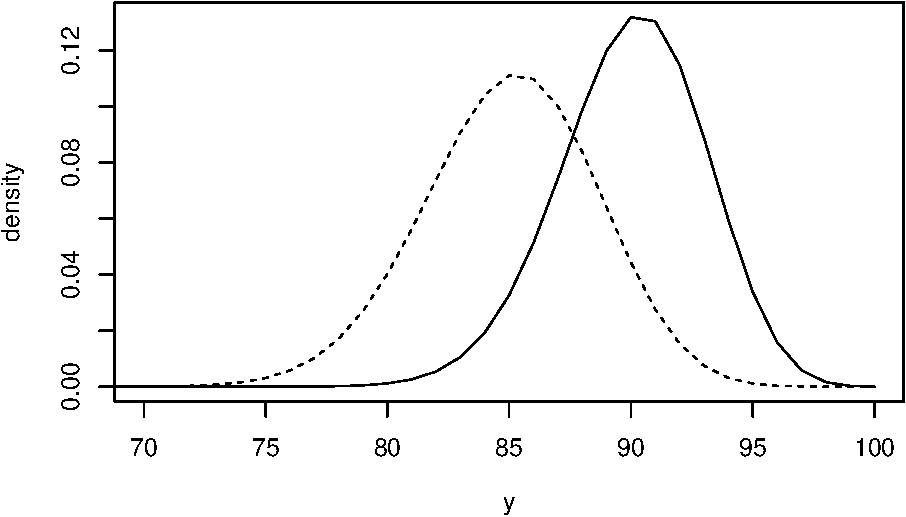
\includegraphics{_main_files/figure-latex/unnamed-chunk-49-1.pdf}

As the variables \(\boldsymbol{z}\) are latent, the observed data likelihood function is
\[
\pi(\boldsymbol{y} \mid  p, \theta_1, \theta_2) =\prod_{i=1}^N \left[ p\pi(y_i \mid p = \theta_1) + (1-p)\pi(y_i \mid \theta_2)\right].
\]
Instead, it's easier to work with the complete data likelihood function, supposing we had observed the variables \(\boldsymbol{z}\). This is given by
\begin{align*}
\pi(\boldsymbol{y}, \boldsymbol{z} \mid  p, \theta_1, \theta_2) &= \pi(\boldsymbol{y} \mid  \boldsymbol{z}, \theta_1, \theta_2)\pi(\boldsymbol{z} \mid p)
\propto p^{N_1}(1-p)^{N_2} \prod_{i; z_i = 1}\pi(y_i \mid \theta_1)\prod_{i; z_i = 2}\pi(y_i \mid \theta_2)
\end{align*}
where \(N_1\) and \(N_2\) are the number of letters for B1 and B2 respectively. This form makes it much easier to derive the posterior distribution, full conditional distributions and estimate the parameter values. By Bayes' theorem, the posterior distribution is
\[
\pi(\boldsymbol{z}, p, \theta_1, \theta_2 \mid \boldsymbol{y}) \propto \pi(\boldsymbol{y} \mid  \boldsymbol{z}, \theta_1, \theta_2)\pi(\boldsymbol{z} \mid p)\pi(p)\pi(\theta_1)\pi(\theta_2). 
\]
Note that we do not put a prior distribution on the latent variables \(\boldsymbol{z}\). Instead, we learn about these variables in the terms \(\pi(\boldsymbol{y} \mid \boldsymbol{z}, \theta_1, \theta_2)\pi(\boldsymbol{z} \mid p)\).

We suppose we are ignorant about the value of \(p\) and place a uniform prior distribution on the parameter \(p\). The full conditional distribution is
\begin{align*}
\pi(p\mid \boldsymbol{z}, \boldsymbol{y}, \theta_1, \theta_2) &\propto \pi(\boldsymbol{z} \mid p)\pi(p)\\
& = p^{N_1}(1-p)^{N_2}.
\end{align*}
Hence,
\[
p \mid \boldsymbol{y}, \boldsymbol{z} \sim \hbox{Beta}(N_1 + 1, N_2 + 1).
\]
If we use a Beta(\(\alpha_1, \beta_1\)) distribution for our prior distribution on \(\theta_1\), the full conditional distribution of \(\theta_1\) is
\begin{align*}
\pi(\theta_1 \mid \boldsymbol{z}, \boldsymbol{y}, \theta_2) \propto pi(\boldsymbol{y} \mid  \boldsymbol{z}, \theta_1, \theta_2)\pi(\theta_1) \\
&\propto \theta_1^{\sum_{i; z_i = 1}y_i}(1-\theta_1)^{100N_1 - \sum_{i; z_i = 1}y_i}\theta^{\alpha_1 - 1}(1-\theta^{\beta_1 - 1}) \\
& \propto \theta_1^{\sum_{i; z_i = 1}y_i + \alpha_1 -1 }(1-\theta_1)^{100N_1 + \beta_1 - \sum_{i; z_i = 1}y_i - 1}
\end{align*}
Hence \(\theta_1 \mid \boldsymbol{z}, \boldsymbol{y}, \theta_2 \sim \hbox{Beta}(\sum_{i; z_i = 1}y_i + \alpha_1 , 100N_1 + \beta_1 - \sum_{i; z_i = 1}y_i)\). Similarly, \(\theta_2 \mid \boldsymbol{z}, \boldsymbol{y}, \theta_1 \sim \hbox{Beta}(\sum_{i; z_i = 2}y_i + \alpha_2 , 100N_2 + \beta_2 - \sum_{i; z_i = 2}y_i)\).

The distribution of \(z_i\) given the parameters \(p\), \(\theta_1\) and \(\theta_2\), and the observation \(y_i\) is
\begin{align*}
p^*_i & = \pi(z = 1 \mid p, y_1) \\
&= \frac{p\pi(y_i \mid \theta_1)}{p\pi(y_i \mid \theta_1) + (1-p)\pi(y_i \mid \theta_2)}.
\end{align*}
Similarly,
\begin{align*}
\pi(z = 2 \mid p, y_1) \\
&= \frac{(1-p)\pi(y_i \mid \theta_2)}{p\pi(y_i \mid \theta_1) + (1-p)\pi(y_i \mid \theta_2)}.
\end{align*}
The full conditional distribution is therefore \(z_i \mid \boldsymbol{y}, p \sim \hbox{Bernoulli}(p^*_i)\).

An MCMC algorithm for this would repeat the following two steps:

\begin{enumerate}
\def\labelenumi{\arabic{enumi}.}
\tightlist
\item
  Initialise values for \(p, \theta_1, \theta_2\) and \(\boldsymbol{z}\)
\item
  Sample \(p \mid \boldsymbol{y}, \boldsymbol{z} \sim \hbox{Beta}(N_1 + 1, N_2 + 1)\).
\item
  Sample \(\theta_1 \mid \boldsymbol{z}, \boldsymbol{y}, \theta_2 \sim\hbox{Beta}(\sum_{i; z_i = 1}y_i + \alpha_1 , 100N_1 + \beta_1 - \sum_{i; z_i = 1}y_i)\).
\item
  Sample \(\theta_2 \mid \boldsymbol{z}, \boldsymbol{y}, \theta_1 \sim \hbox{Beta}(\sum_{i; z_i = 2}y_i + \alpha_2 , 100N_2 + \beta_2 - \sum_{i; z_i = 2}y_i)\).
\item
  Sample \(z_i \mid \boldsymbol{y}, p \sim \hbox{Bernoulli}(p^*_i)\) for each \(i\).
\item
  Repeat Steps 3-5.
\end{enumerate}

This algorithm may be very slow to converge and explore the posterior distribution. This is because it has so many parameters. There is 3 model parameters (\(p\), \(\beta_1\) and \(\beta_2\)) and \(N\) latent variables. Exploring a posterior distribution with this many dimensions may take a lot of time. Royal Mail delivered \textasciitilde20,000,000 letters a day in 2023.
\end{example}

\hypertarget{grouped-data}{%
\subsection{Grouped Data}\label{grouped-data}}

Often, we can only receive data in grouped form. This is often the case in medical and crime settings, where patients are grouped together to protect their identity. Grouping data introduces a difficulty when trying to perform inference. Augmenting the data, by introducing parameters to represent different parts of the group can both simplify the inference workflow and provide more information than is possible otherwise.

\begin{example}
Suppose that we have data on the number of treatment sessions required by a random sample of patients before they recover from a disease. For identifiability reasons, the numbers of patients requiring two or fewer treatment sessions are grouped and we obtain the following table

\begin{longtable}[]{@{}llllll@{}}
\toprule\noalign{}
Number of sessions \(x\) & \(\leq 2\) & 3 & 4 & 5 & 6 \\
\midrule\noalign{}
\endhead
\bottomrule\noalign{}
\endlastfoot
Frequency \(f(x)\) & 25 & 7 & 4 & 3 & 1 \\
\end{longtable}

We are interested the the probability the treatment sessions are a success. We can model this using the geometric distribution, assuming each treatment session is independent and has probability of success is \(p\). For each group of patients, we can work out their contribution to the observed likelihood function using a geometric distribution. For example, the contribution to the likelihood function for patients who had three treatment sessions is \(((1-p)^2p)^7\). For the group that had two or fewer sessions, the likelihood contribution is \((1-(1-p))^{25}\). The observed likelihood function is therefore
\begin{align*}
\pi(f_{1, 2}, f_3, \ldots, f_6 \mid p) &= (1-(1-p))^{25}(1-p)^{43}p^{15} \\
&= p^{40}(1-p)^{43}(2-p)^{25}
\end{align*}
There is no conjugate prior distribution that induces conjugacy. We use the prior distribution \(p \sim \hbox{Beta}(\alpha, \beta)\).By Bayes' theorem, the posterior distribution is
\[
\pi(p \mid f_{1, 2}, f_3, \ldots, f_6 ) \propto p^{40 + \alpha - 1}(1-p)^{43 + \beta - 1}(2-p)^{25}.
\]

We can use a Metropolis-Hasting algorithm to sample from this algorithm. A suitable algorithm would look like this

\begin{enumerate}
\def\labelenumi{\arabic{enumi}.}
\tightlist
\item
  Initialize \(p^{(0)}\) and \(i = 1\).
\item
  Propose \(p' \sim U[p^{(i)} + \varepsilon, p^{(i)} - \varepsilon]\).
\item
  Accept \(p^{(i+1)}=p'\) with probability \(p_{acc}\), otherwise reject as set \(p^{(i+1)}=p^{(i)}\).
\item
  Set \(i=i+1\) and repeat steps 2-3.
\end{enumerate}

The acceptance probability in step 3 is given by
\[
p_{\textrm{acc}} = \min\left\{\frac{p'^{40 + \alpha - 1}(1-p')^{43 + \beta - 1}(2-p')^{25}}{p^{40 + \alpha - 1}(1-p)^{43 + \beta - 1}(2-p)^{25}} ,1\right\}
\]
Instead of using the observed likelihood, we can write the complete likelihood function supposing we had seen the number of patients who had had one and two sessions. The complete likelihood function is
\[
\pi(f_1 \ldots, f_6 \mid p) = p^{40}(1-p)^{\sum f(x) - 40}. 
\]
Now, the Beta(\(\alpha, \beta)\) prior distribution is conjugate and we have
\[
p \mid f_1 \ldots, f_6  \sim \hbox{Beta}(40 + \alpha, \sum f(x) - 40 + \beta).
\]
Now, we need to derive the full conditional distribution for \(f(1)\), the number of patients who were treated after only one sessions, \(\pi(f_1 \mid p, f_{1, 2}, f_3, \ldots, f_6)\). Under the geometric distribution model, the probability a patient is treated after exactly one session is \(p\) and after two sessions is \((1-p)p\). We can use these probabilities in a Binomial distribution. We have 25 patients each with a probability of being treated \(q\), where
\[
q = \frac{p}{p + (1-p)p}
\]
Therefore \(f_1 \mid p, f_{1, 2}, f_3, \ldots, f_6 \sim \hbox{Bin}(25, q)\). We do not need to sample \(f_2\) as we have \(f_2 = 25 - f_1\). Our MCMC algorithm using the complete data likelihood function and inferring \(f_1\) and \(f_2\) as well as \(p\) could be

\begin{enumerate}
\def\labelenumi{\arabic{enumi}.}
\tightlist
\item
  Initialise \(p^{(0)}\), \(f_1^{(0)}\) and \(f_2^{(0)}\). Set \(i = 1\).
\item
  Sample \(p^{(i)} \mid f_1^{(i-1)}, f_2^{(i-1)}, f_3 \ldots, f_6 \sim \hbox{Beta}(40 + \alpha, \sum f(x) - 40 + \beta)\)
\item
  Sample \$f\_1\^{}\{(i)\} \mid p\^{}\{(i)\}, f\_\{1, 2\}, f\_3, \ldots, f\_6 \$
\item
  Compute \(f_2^{(i)} = 25 - f_1^{(i)}\).
\item
  Repeat steps 2 - 4.
\end{enumerate}

This MCMC algorithm avoids us needing to do any tuning or accept/reject steps, making it more efficient.
\end{example}

\hypertarget{approximate-bayesian-computation}{%
\section{Approximate Bayesian Computation}\label{approximate-bayesian-computation}}

So far, we have always considered models where the likelihood function is easy to work with. By easy, we mean that we can evaluate the likelihood function for lots of different values, and we can evaluate it cheaply. In some cases, it might not be possible to write down the likelihood function, or it might not be possible to evaluate it. In these cases, we refer to methods call \textbf{likelihood free inference}.

\begin{example}
Models to predict the weather are notoriously complex. They contain a huge number of parameters, and sometimes it is not possible to write this model down exactly. In cases where the likelihood function for the weather model can be written down, we would have to start the MCMC algorithm from scratch every time we collected new data.
\end{example}

Approximate Bayesian Computation (ABC) is a likelihood free algorithm that relies on reject sampling from the prior distribution. When constructing an ABC algorithm, we only need to be able to generate data given a parameter value and not evaluate the likelihood of seeing specific data given a parameter value.

We are going to look at two types of ABC. The first is ABC with rejection

\hypertarget{abc-with-rejection}{%
\subsection{ABC with Rejection}\label{abc-with-rejection}}

\begin{definition}

To carry out inference for a parameter \(\theta\) using an Approximate Bayesian Computation algorithm with rejection

\begin{enumerate}
\def\labelenumi{\arabic{enumi}.}
\tightlist
\item
  Sample a value for the parameter \(\theta^*\) from the prior distribution \(\pi(\theta)\).
\item
  Generate some data \(y*\) from the data generating process using the parameter value \(\theta^*\).
\item
  Accept \(\theta^*\) as a value from the posterior distribution if \(||y - y^*|| < \varepsilon\) for some \(\varepsilon > 0\). Otherwise reject \(\theta^*\)
\item
  Repeat steps 1 - 3.
\end{enumerate}

\end{definition}

\begin{definition}
The approximate posterior distribution using ABC with rejection is
\[
\pi_\varepsilon(\theta \mid y) \propto \int \pi(y^* \mid \theta^*)\pi(\theta^*)I_{A_\varepsilon(y^*)} dy^*,
\]
where \({A_\varepsilon(y^*)} = \{y^* \mid ||y^* - y||< \varepsilon\}\).
\end{definition}

\begin{example}

This is a simple example, where we can derive the posterior distribution, but it allows us to see how this method works. Suppose we observe \(Y_1, \ldots, y_510\sim Beta(3, \beta)\). We place a uniform prior on \(\beta\) such that \(\beta \sim U[0, 5]\). The ABC algorithm with rejection works as follows:

\begin{enumerate}
\def\labelenumi{\arabic{enumi}.}
\tightlist
\item
  Sample a value \(\beta^* \sim U[0, 5]\).
\item
  Simulate \(y^*_1, \ldots, y^*_10 \sim Beta(3,\beta^*)\)
\item
  Compute \(D = \sum_{i=1}^{10}(y_i -y^*_i)^2\). If \(D < 0.75\), accept \(\beta^*\) as a sample from the posterior distribution. Otherwise, reject \(\beta^*\).
\item
  Repeat steps 1, 2, and 3.
\end{enumerate}

The code below carries out this algorithm.

\begin{Shaded}
\begin{Highlighting}[]
\CommentTok{\#Set Up Example}
\FunctionTok{set.seed}\NormalTok{(}\DecValTok{1234}\NormalTok{)}
\NormalTok{n }\OtherTok{\textless{}{-}} \DecValTok{10}
\NormalTok{y }\OtherTok{\textless{}{-}} \FunctionTok{rbeta}\NormalTok{(n, }\DecValTok{3}\NormalTok{, }\DecValTok{2}\NormalTok{)}
\NormalTok{y}
\end{Highlighting}
\end{Shaded}

\begin{verbatim}
##  [1] 0.8519237 0.5286251 0.3126172 0.9691679 0.4883547 0.4677043 0.7339799
##  [8] 0.7279578 0.7317827 0.7971786
\end{verbatim}

\begin{Shaded}
\begin{Highlighting}[]
\CommentTok{\#Set Up ABC}
\NormalTok{n.iter }\OtherTok{\textless{}{-}} \DecValTok{50000}
\NormalTok{b.store }\OtherTok{\textless{}{-}} \FunctionTok{numeric}\NormalTok{(n.iter)}
\NormalTok{epsilon }\OtherTok{\textless{}{-}} \FloatTok{0.75}

\CommentTok{\#Run ABC}
\ControlFlowTok{for}\NormalTok{(i }\ControlFlowTok{in} \DecValTok{1}\SpecialCharTok{:}\NormalTok{n.iter)\{}
  
  \CommentTok{\#Propose new beta}
\NormalTok{  b }\OtherTok{\textless{}{-}} \FunctionTok{runif}\NormalTok{(}\DecValTok{1}\NormalTok{, }\DecValTok{0}\NormalTok{, }\DecValTok{5}\NormalTok{)}
  
  \CommentTok{\#Simualate data}
\NormalTok{  y.star }\OtherTok{\textless{}{-}} \FunctionTok{rbeta}\NormalTok{(n, }\DecValTok{3}\NormalTok{, b)}
  
  \CommentTok{\#Compute statistic}
\NormalTok{  d }\OtherTok{\textless{}{-}} \FunctionTok{sum}\NormalTok{((y}\SpecialCharTok{{-}}\NormalTok{y.star)}\SpecialCharTok{\^{}}\DecValTok{2}\NormalTok{)}
  
  \CommentTok{\#Accept/Reject}
  \ControlFlowTok{if}\NormalTok{(d }\SpecialCharTok{\textless{}}\NormalTok{ epsilon)\{}
\NormalTok{    b.store[i] }\OtherTok{\textless{}{-}}\NormalTok{ b}
\NormalTok{  \} }\ControlFlowTok{else}\NormalTok{\{}
\NormalTok{    b.store[i] }\OtherTok{\textless{}{-}} \ConstantTok{NA}
\NormalTok{  \}}
  
\NormalTok{\}}

\CommentTok{\#Get number of reject samples}
\FunctionTok{sum}\NormalTok{(}\FunctionTok{is.na}\NormalTok{(b.store))}
\end{Highlighting}
\end{Shaded}

\begin{verbatim}
## [1] 37886
\end{verbatim}

\begin{Shaded}
\begin{Highlighting}[]
\CommentTok{\#Plot Approximate Posterior}
\FunctionTok{hist}\NormalTok{(b.store, }\AttributeTok{freq =} \ConstantTok{FALSE}\NormalTok{, }\AttributeTok{xlab =} \FunctionTok{expression}\NormalTok{(beta), }\AttributeTok{main =} \StringTok{""}\NormalTok{)}
\FunctionTok{abline}\NormalTok{(}\AttributeTok{v =} \DecValTok{2}\NormalTok{, }\AttributeTok{col =} \StringTok{\textquotesingle{}red\textquotesingle{}}\NormalTok{)}
\end{Highlighting}
\end{Shaded}

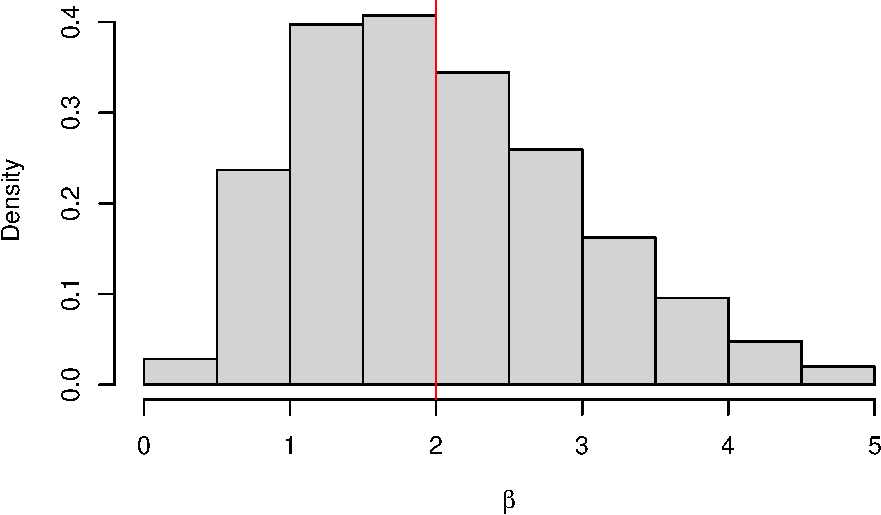
\includegraphics{_main_files/figure-latex/unnamed-chunk-50-1.pdf}

\begin{Shaded}
\begin{Highlighting}[]
\FunctionTok{mean}\NormalTok{(b.store, }\AttributeTok{na.rm =} \ConstantTok{TRUE}\NormalTok{)}
\end{Highlighting}
\end{Shaded}

\begin{verbatim}
## [1] 2.03304
\end{verbatim}

\begin{Shaded}
\begin{Highlighting}[]
\FunctionTok{quantile}\NormalTok{(b.store, }\FunctionTok{c}\NormalTok{(}\FloatTok{0.025}\NormalTok{, }\FloatTok{0.975}\NormalTok{), }\AttributeTok{na.rm =} \ConstantTok{TRUE}\NormalTok{)}
\end{Highlighting}
\end{Shaded}

\begin{verbatim}
##      2.5%     97.5% 
## 0.5843792 4.1369339
\end{verbatim}

\end{example}

One important question is how to choose the value for \(\varepsilon\)? It turns out this is an incredibly hard question that is specific to each application. Often the approximate posterior distribution \(\pi_\varepsilon(\theta \mid y)\) is very sensitive to the choice of \(\varepsilon\).

\begin{example}

Let's repeat the example, first with \(\varepsilon = 0.12\). In this case, almost all of the proposals are rejected.

\begin{Shaded}
\begin{Highlighting}[]
\CommentTok{\#Set Up Example}
\FunctionTok{set.seed}\NormalTok{(}\DecValTok{1234}\NormalTok{)}
\NormalTok{n }\OtherTok{\textless{}{-}} \DecValTok{10}
\NormalTok{y }\OtherTok{\textless{}{-}} \FunctionTok{rbeta}\NormalTok{(n, }\DecValTok{3}\NormalTok{, }\DecValTok{2}\NormalTok{)}
\NormalTok{y}
\end{Highlighting}
\end{Shaded}

\begin{verbatim}
##  [1] 0.8519237 0.5286251 0.3126172 0.9691679 0.4883547 0.4677043 0.7339799
##  [8] 0.7279578 0.7317827 0.7971786
\end{verbatim}

\begin{Shaded}
\begin{Highlighting}[]
\CommentTok{\#Set Up ABC}
\NormalTok{n.iter }\OtherTok{\textless{}{-}} \DecValTok{50000}
\NormalTok{b.store }\OtherTok{\textless{}{-}} \FunctionTok{numeric}\NormalTok{(n.iter)}
\NormalTok{epsilon }\OtherTok{\textless{}{-}} \FloatTok{0.12}

\CommentTok{\#Run ABC}
\ControlFlowTok{for}\NormalTok{(i }\ControlFlowTok{in} \DecValTok{1}\SpecialCharTok{:}\NormalTok{n.iter)\{}
  
  \CommentTok{\#Propose new beta}
\NormalTok{  b }\OtherTok{\textless{}{-}} \FunctionTok{runif}\NormalTok{(}\DecValTok{1}\NormalTok{, }\DecValTok{0}\NormalTok{, }\DecValTok{5}\NormalTok{)}
  
  \CommentTok{\#Simualate data}
\NormalTok{  y.star }\OtherTok{\textless{}{-}} \FunctionTok{rbeta}\NormalTok{(n, }\DecValTok{3}\NormalTok{, b)}
  
  \CommentTok{\#Compute statistic}
\NormalTok{  d }\OtherTok{\textless{}{-}} \FunctionTok{sum}\NormalTok{((y}\SpecialCharTok{{-}}\NormalTok{y.star)}\SpecialCharTok{\^{}}\DecValTok{2}\NormalTok{)}
  
  \CommentTok{\#Accept/Reject}
  \ControlFlowTok{if}\NormalTok{(d }\SpecialCharTok{\textless{}}\NormalTok{ epsilon)\{}
\NormalTok{    b.store[i] }\OtherTok{\textless{}{-}}\NormalTok{ b}
\NormalTok{  \} }\ControlFlowTok{else}\NormalTok{\{}
\NormalTok{    b.store[i] }\OtherTok{\textless{}{-}} \ConstantTok{NA}
\NormalTok{  \}}
  
\NormalTok{\}}

\CommentTok{\#Get number of reject samples}
\FunctionTok{sum}\NormalTok{(}\FunctionTok{is.na}\NormalTok{(b.store))}
\end{Highlighting}
\end{Shaded}

\begin{verbatim}
## [1] 49993
\end{verbatim}

\begin{Shaded}
\begin{Highlighting}[]
\CommentTok{\#Plot Approximate Posterior}
\FunctionTok{hist}\NormalTok{(b.store, }\AttributeTok{freq =} \ConstantTok{FALSE}\NormalTok{, }\AttributeTok{xlab =} \FunctionTok{expression}\NormalTok{(beta), }\AttributeTok{main =} \StringTok{""}\NormalTok{)}
\FunctionTok{abline}\NormalTok{(}\AttributeTok{v =} \DecValTok{2}\NormalTok{, }\AttributeTok{col =} \StringTok{\textquotesingle{}red\textquotesingle{}}\NormalTok{)}
\end{Highlighting}
\end{Shaded}

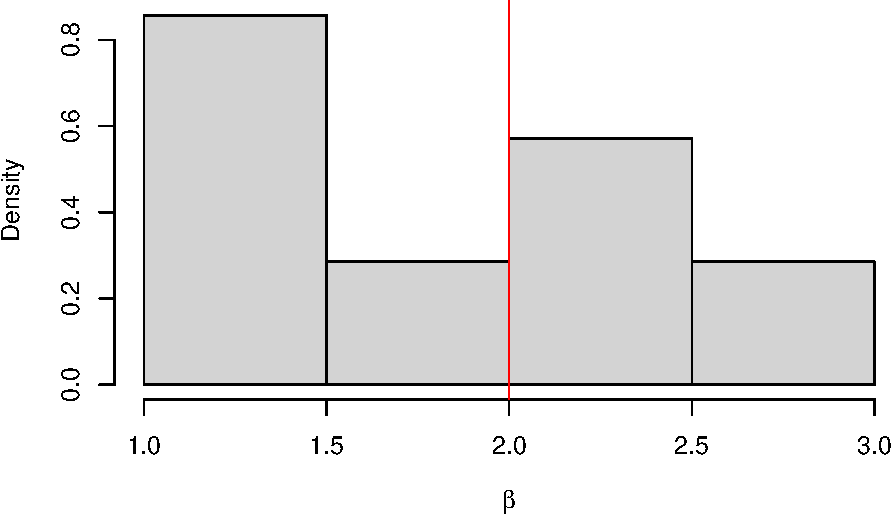
\includegraphics{_main_files/figure-latex/unnamed-chunk-51-1.pdf}

\begin{Shaded}
\begin{Highlighting}[]
\FunctionTok{mean}\NormalTok{(b.store, }\AttributeTok{na.rm =} \ConstantTok{TRUE}\NormalTok{)}
\end{Highlighting}
\end{Shaded}

\begin{verbatim}
## [1] 1.831118
\end{verbatim}

\begin{Shaded}
\begin{Highlighting}[]
\FunctionTok{quantile}\NormalTok{(b.store, }\FunctionTok{c}\NormalTok{(}\FloatTok{0.025}\NormalTok{, }\FloatTok{0.975}\NormalTok{), }\AttributeTok{na.rm =} \ConstantTok{TRUE}\NormalTok{)}
\end{Highlighting}
\end{Shaded}

\begin{verbatim}
##     2.5%    97.5% 
## 1.181349 2.587056
\end{verbatim}

\end{example}

\begin{example}
And now again with \(\varepsilon = 2\). In this case, almost all of the proposals are accepted.

\begin{Shaded}
\begin{Highlighting}[]
\CommentTok{\#Set Up Example}
\FunctionTok{set.seed}\NormalTok{(}\DecValTok{1234}\NormalTok{)}
\NormalTok{n }\OtherTok{\textless{}{-}} \DecValTok{10}
\NormalTok{y }\OtherTok{\textless{}{-}} \FunctionTok{rbeta}\NormalTok{(n, }\DecValTok{3}\NormalTok{, }\DecValTok{2}\NormalTok{)}
\NormalTok{y}
\end{Highlighting}
\end{Shaded}

\begin{verbatim}
##  [1] 0.8519237 0.5286251 0.3126172 0.9691679 0.4883547 0.4677043 0.7339799
##  [8] 0.7279578 0.7317827 0.7971786
\end{verbatim}

\begin{Shaded}
\begin{Highlighting}[]
\CommentTok{\#Set Up ABC}
\NormalTok{n.iter }\OtherTok{\textless{}{-}} \DecValTok{50000}
\NormalTok{b.store }\OtherTok{\textless{}{-}} \FunctionTok{numeric}\NormalTok{(n.iter)}
\NormalTok{epsilon }\OtherTok{\textless{}{-}} \DecValTok{2}

\CommentTok{\#Run ABC}
\ControlFlowTok{for}\NormalTok{(i }\ControlFlowTok{in} \DecValTok{1}\SpecialCharTok{:}\NormalTok{n.iter)\{}
  
  \CommentTok{\#Propose new beta}
\NormalTok{  b }\OtherTok{\textless{}{-}} \FunctionTok{runif}\NormalTok{(}\DecValTok{1}\NormalTok{, }\DecValTok{0}\NormalTok{, }\DecValTok{5}\NormalTok{)}
  
  \CommentTok{\#Simualate data}
\NormalTok{  y.star }\OtherTok{\textless{}{-}} \FunctionTok{rbeta}\NormalTok{(n, }\DecValTok{3}\NormalTok{, b)}
  
  \CommentTok{\#Compute statistic}
\NormalTok{  d }\OtherTok{\textless{}{-}} \FunctionTok{sum}\NormalTok{((y}\SpecialCharTok{{-}}\NormalTok{y.star)}\SpecialCharTok{\^{}}\DecValTok{2}\NormalTok{)}
  
  \CommentTok{\#Accept/Reject}
  \ControlFlowTok{if}\NormalTok{(d }\SpecialCharTok{\textless{}}\NormalTok{ epsilon)\{}
\NormalTok{    b.store[i] }\OtherTok{\textless{}{-}}\NormalTok{ b}
\NormalTok{  \} }\ControlFlowTok{else}\NormalTok{\{}
\NormalTok{    b.store[i] }\OtherTok{\textless{}{-}} \ConstantTok{NA}
\NormalTok{  \}}
  
\NormalTok{\}}

\CommentTok{\#Get number of reject samples}
\FunctionTok{sum}\NormalTok{(}\FunctionTok{is.na}\NormalTok{(b.store))}
\end{Highlighting}
\end{Shaded}

\begin{verbatim}
## [1] 471
\end{verbatim}

\begin{Shaded}
\begin{Highlighting}[]
\CommentTok{\#Plot Approximate Posterior}
\FunctionTok{hist}\NormalTok{(b.store, }\AttributeTok{freq =} \ConstantTok{FALSE}\NormalTok{, }\AttributeTok{xlab =} \FunctionTok{expression}\NormalTok{(beta), }\AttributeTok{main =} \StringTok{""}\NormalTok{)}
\FunctionTok{abline}\NormalTok{(}\AttributeTok{v =} \DecValTok{2}\NormalTok{, }\AttributeTok{col =} \StringTok{\textquotesingle{}red\textquotesingle{}}\NormalTok{)}
\end{Highlighting}
\end{Shaded}

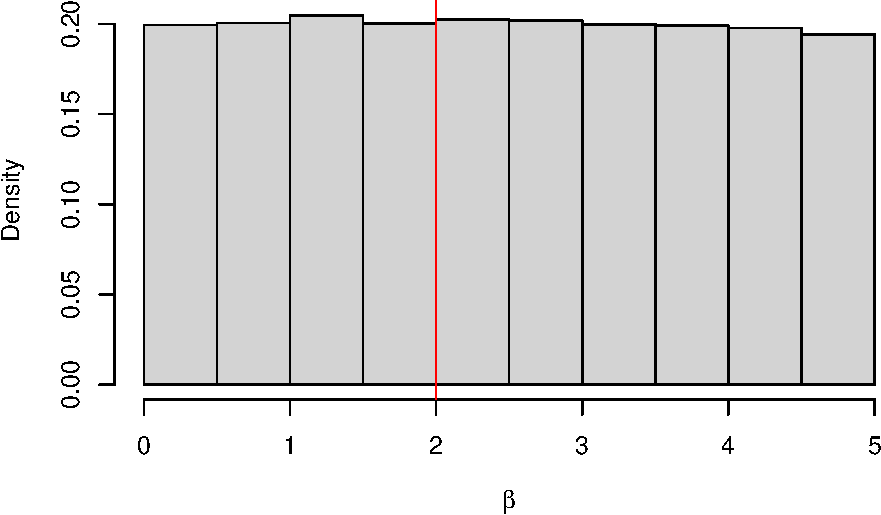
\includegraphics{_main_files/figure-latex/unnamed-chunk-52-1.pdf}

\begin{Shaded}
\begin{Highlighting}[]
\FunctionTok{mean}\NormalTok{(b.store, }\AttributeTok{na.rm =} \ConstantTok{TRUE}\NormalTok{)}
\end{Highlighting}
\end{Shaded}

\begin{verbatim}
## [1] 2.488073
\end{verbatim}

\begin{Shaded}
\begin{Highlighting}[]
\FunctionTok{quantile}\NormalTok{(b.store, }\FunctionTok{c}\NormalTok{(}\FloatTok{0.025}\NormalTok{, }\FloatTok{0.975}\NormalTok{), }\AttributeTok{na.rm =} \ConstantTok{TRUE}\NormalTok{)}
\end{Highlighting}
\end{Shaded}

\begin{verbatim}
##      2.5%     97.5% 
## 0.1281937 4.8666030
\end{verbatim}

When \(\varepsilon = 0.12\), almost all the proposals are rejected. Although the approximate posterior mean is close to the true value, given we only have 7 samples we cannot say much about the posterior distribution. When \(\varepsilon = 2\), almost all the proposals are accepted. This histogram shows that we are really just sampling from the prior distribution, i.e.~\(\pi_2(\beta \mid y) \approx \pi(\beta)\).
\end{example}

\begin{proposition}
Using an ABC rejection algorithm
\[
\lim_{\varepsilon \rightarrow \infty} \pi_\varepsilon(\theta \mid y) \overset{D}= \pi(\theta),
\]
and
\[
\lim_{\varepsilon \rightarrow 0} \pi_\varepsilon(\theta \mid y) \overset{D}= \pi(\theta \mid y). 
\]
\end{proposition}

\begin{proof}
See problem sheet.
\end{proof}

This example and the proposition show that if we set \(\varepsilon\) too large, we don't learn anything about \(\theta\), we just recover the data. The smaller the value of \(\varepsilon\), the better. But very small values may require very long run times, or have such few samples that the noise from the sampling generator is larger than the signal in the accepted samples. The only diagnostic tools we have are the proportion of samples accepted and the histograms of the approximate posterior and prior distributions.

\begin{example}

An example of where this is useful is epidemic modelling. Suppose we have a population of 100 individuals and at each time point an individual is Susceptible to a disease, Infected with the disease, or Recovered and therefore immune. Once infected with the disease, an individual infects people according to a Poisson process with rate \(\beta\). Each infected person is infected from a time period drawn from an Exponential distribution with rate \(1\). We observe the total number of people infected with the disease at the end of the outbreak. To carry out inference for the infection rate \(\beta\), we need to use the augmented likelihood function The augmented likelihood function for this model is given by

\[
\pi(\textbf{i}, \textbf{r}| \beta) \propto \underbrace{\exp\Big(- \sum\limits_{j=1}^n\sum\limits_{k=1}^N \beta\big((r_j \wedge i_k) - (i_j \wedge i_k)\big)\Big)}_\text{Avoiding infection} \\
 \times\hspace{1.8cm} \underbrace{\prod\limits_{\substack{j=1 \\ j \neq \kappa}}^n\Big(\sum\limits_{k \in \mathcal{Y}_j} \beta\Big)}_\text{Becoming infectious}  \\
\times \hspace{1.8cm}\underbrace{\prod\limits_{j=1}^n\pi(r_j -i_j | \gamma = 1)}_\text{Remaining infected}.
\]
This likelihood function cannot be evaluated as we do not observe the infection time \(i\) or recovery time \(r\). Instead we can use ABC sampling with rejection. Each iteration, sample a value for \(\beta\), simulate an outbreak and compare the observed and simulated number of people infected. If they are `close' we accept the value for \(\beta\) as a sample from our posterior distribution. This means all we have to do is simulate outbreaks.

\begin{Shaded}
\begin{Highlighting}[]
\CommentTok{\#This function simualtes an outbreak of a disease in a population of size N, with infection rate beta and recovery rate gamma.}
\NormalTok{simSIR.Markov }\OtherTok{\textless{}{-}} \ControlFlowTok{function}\NormalTok{(N, beta, gamma) \{}
  
  \CommentTok{\# initial number of infectives and susceptibles;}
\NormalTok{  I }\OtherTok{\textless{}{-}} \DecValTok{1}
\NormalTok{  S }\OtherTok{\textless{}{-}}\NormalTok{ N}\DecValTok{{-}1}\NormalTok{;}
  
  \CommentTok{\# recording time;}
\NormalTok{  t }\OtherTok{\textless{}{-}} \DecValTok{0}\NormalTok{;}
\NormalTok{  times }\OtherTok{\textless{}{-}} \FunctionTok{c}\NormalTok{(t);}
  
  \CommentTok{\# a vector which records the type of event (1=infection, 2=removal)}
\NormalTok{  type }\OtherTok{\textless{}{-}} \FunctionTok{c}\NormalTok{(}\DecValTok{1}\NormalTok{);}
  
  \ControlFlowTok{while}\NormalTok{ (I }\SpecialCharTok{\textgreater{}} \DecValTok{0}\NormalTok{) \{}
    
    \CommentTok{\# time to next event;}
\NormalTok{    t }\OtherTok{\textless{}{-}}\NormalTok{ t }\SpecialCharTok{+} \FunctionTok{rexp}\NormalTok{(}\DecValTok{1}\NormalTok{, (beta}\SpecialCharTok{/}\NormalTok{N)}\SpecialCharTok{*}\NormalTok{I}\SpecialCharTok{*}\NormalTok{S }\SpecialCharTok{+}\NormalTok{ gamma}\SpecialCharTok{*}\NormalTok{I);}
\NormalTok{    times }\OtherTok{\textless{}{-}} \FunctionTok{append}\NormalTok{(times, t);}
    
    \ControlFlowTok{if}\NormalTok{ (}\FunctionTok{runif}\NormalTok{(}\DecValTok{1}\NormalTok{) }\SpecialCharTok{\textless{}}\NormalTok{ beta}\SpecialCharTok{*}\NormalTok{S}\SpecialCharTok{/}\NormalTok{(beta}\SpecialCharTok{*}\NormalTok{S }\SpecialCharTok{+}\NormalTok{ N}\SpecialCharTok{*}\NormalTok{gamma)) \{}
      \CommentTok{\# infection}
\NormalTok{      I }\OtherTok{\textless{}{-}}\NormalTok{ I}\SpecialCharTok{+}\DecValTok{1}\NormalTok{;}
\NormalTok{      S }\OtherTok{\textless{}{-}}\NormalTok{ S}\DecValTok{{-}1}\NormalTok{;}
\NormalTok{      type }\OtherTok{\textless{}{-}} \FunctionTok{append}\NormalTok{(type, }\DecValTok{1}\NormalTok{);}
\NormalTok{    \}}
    \ControlFlowTok{else}\NormalTok{ \{}
      \CommentTok{\#removal}
\NormalTok{      I }\OtherTok{\textless{}{-}}\NormalTok{ I}\DecValTok{{-}1}
\NormalTok{      type }\OtherTok{\textless{}{-}} \FunctionTok{append}\NormalTok{(type, }\DecValTok{2}\NormalTok{);}
\NormalTok{    \}}
\NormalTok{  \}}
  
  
  \CommentTok{\# record the times of events (infections/removals), the type of the event, the final size (including}
  \CommentTok{\# the initial infective) and the duration. }
  
\NormalTok{  res }\OtherTok{\textless{}{-}} \FunctionTok{list}\NormalTok{(}\StringTok{"t"} \OtherTok{=}\NormalTok{ times, }\StringTok{"type"} \OtherTok{=}\NormalTok{ type, }\StringTok{"final.size"} \OtherTok{=} \FunctionTok{sum}\NormalTok{(type}\SpecialCharTok{==}\DecValTok{1}\NormalTok{), }\StringTok{"duration"} \OtherTok{=}\NormalTok{ t, }\StringTok{"N"} \OtherTok{=}\NormalTok{ N);}
  \FunctionTok{return}\NormalTok{(res)}
\NormalTok{\}}

\CommentTok{\#Set Up Example}
\FunctionTok{set.seed}\NormalTok{(}\DecValTok{1234}\NormalTok{)}
\NormalTok{n }\OtherTok{\textless{}{-}} \DecValTok{200}
\NormalTok{y }\OtherTok{\textless{}{-}} \FunctionTok{simSIR.Markov}\NormalTok{(}\DecValTok{100}\NormalTok{, }\DecValTok{2}\NormalTok{, }\DecValTok{1}\NormalTok{)}\SpecialCharTok{$}\NormalTok{final.size}


\CommentTok{\#Set Up ABC}
\NormalTok{n.iter }\OtherTok{\textless{}{-}} \DecValTok{50000}
\NormalTok{b.store }\OtherTok{\textless{}{-}} \FunctionTok{numeric}\NormalTok{(n.iter)}
\NormalTok{epsilon }\OtherTok{\textless{}{-}} \DecValTok{250}

\CommentTok{\#Run ABC}
\ControlFlowTok{for}\NormalTok{(i }\ControlFlowTok{in} \DecValTok{1}\SpecialCharTok{:}\NormalTok{n.iter)\{}
  
  \CommentTok{\#Propose an infection rate}
\NormalTok{  b }\OtherTok{\textless{}{-}} \FunctionTok{runif}\NormalTok{(}\DecValTok{1}\NormalTok{, }\DecValTok{0}\NormalTok{, }\DecValTok{5}\NormalTok{)}
  
  \CommentTok{\#Simualte an outbreak}
\NormalTok{  y.star }\OtherTok{\textless{}{-}} \FunctionTok{simSIR.Markov}\NormalTok{(}\DecValTok{100}\NormalTok{, b, }\DecValTok{1}\NormalTok{)}\SpecialCharTok{$}\NormalTok{final.size}
  
  \CommentTok{\#Compute difference}
\NormalTok{  d }\OtherTok{\textless{}{-}} \FunctionTok{sum}\NormalTok{((y}\SpecialCharTok{{-}}\NormalTok{y.star)}\SpecialCharTok{\^{}}\DecValTok{2}\NormalTok{)}
  
  \CommentTok{\#Accept/Reject}
  \ControlFlowTok{if}\NormalTok{(d }\SpecialCharTok{\textless{}}\NormalTok{ epsilon)\{}
\NormalTok{    b.store[i] }\OtherTok{\textless{}{-}}\NormalTok{ b}
\NormalTok{  \} }\ControlFlowTok{else}\NormalTok{\{}
\NormalTok{    b.store[i] }\OtherTok{\textless{}{-}} \ConstantTok{NA}
\NormalTok{  \}}
  
\NormalTok{\}}

\CommentTok{\#Get number of reject samples}
\FunctionTok{sum}\NormalTok{(}\FunctionTok{is.na}\NormalTok{(b.store))}
\end{Highlighting}
\end{Shaded}

\begin{verbatim}
## [1] 39166
\end{verbatim}

\begin{Shaded}
\begin{Highlighting}[]
\CommentTok{\#Plot Approximate Posterior}
\FunctionTok{hist}\NormalTok{(b.store, }\AttributeTok{freq =} \ConstantTok{FALSE}\NormalTok{, }\AttributeTok{xlab =} \FunctionTok{expression}\NormalTok{(beta), }\AttributeTok{main =} \StringTok{""}\NormalTok{)}
\FunctionTok{abline}\NormalTok{(}\AttributeTok{v =} \DecValTok{2}\NormalTok{, }\AttributeTok{col =} \StringTok{\textquotesingle{}red\textquotesingle{}}\NormalTok{)}
\end{Highlighting}
\end{Shaded}

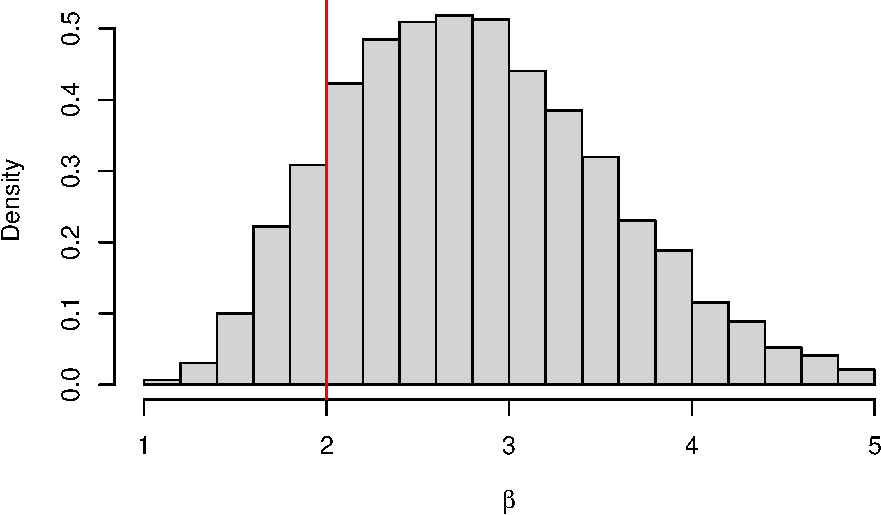
\includegraphics{_main_files/figure-latex/unnamed-chunk-53-1.pdf}

\begin{Shaded}
\begin{Highlighting}[]
\FunctionTok{mean}\NormalTok{(b.store, }\AttributeTok{na.rm =} \ConstantTok{TRUE}\NormalTok{)}
\end{Highlighting}
\end{Shaded}

\begin{verbatim}
## [1] 2.811462
\end{verbatim}

\begin{Shaded}
\begin{Highlighting}[]
\FunctionTok{quantile}\NormalTok{(b.store, }\FunctionTok{c}\NormalTok{(}\FloatTok{0.025}\NormalTok{, }\FloatTok{0.975}\NormalTok{), }\AttributeTok{na.rm =} \ConstantTok{TRUE}\NormalTok{)}
\end{Highlighting}
\end{Shaded}

\begin{verbatim}
##     2.5%    97.5% 
## 1.589679 4.367686
\end{verbatim}

\end{example}

\hypertarget{summary-abc-with-rejection}{%
\subsection{Summary ABC with Rejection}\label{summary-abc-with-rejection}}

ABC with rejection suffers from the curse of dimensionality (see Chapter 5). As the number of data points increases, the probability we get a `close' match decreases. This means we have to increase \(\varepsilon\) and degrade the quality of our approximation.

\begin{example}
Let's repeat the Beta example with \(n = 200\) observed data points. We need \(\varepsilon > 15\) for any proposals to be accepted.
\end{example}

We can avoid the curse of dimensionality by comparing summary statistics instead. This leads us to the Summary ABC algorithm.

\begin{definition}

To carry out inference for a parameter \(\theta\) using an Summary Approximate Bayesian Computation algorithm with rejection

\begin{enumerate}
\def\labelenumi{\arabic{enumi}.}
\tightlist
\item
  Sample a value for the parameter \(\theta^*\) from the prior distribution \(\pi(\theta)\).
\item
  Generate some data \(y*\) from the data generating process using the parameter value \(\theta^*\).
\item
  Accept \(\theta^*\) as a value from the posterior distribution if \(||S(y) - S(y^*)|| < \varepsilon\) for some \(\varepsilon > 0\) and summary summary statistic \(S\). Otherwise reject \(\theta^*\)
\item
  Repeat steps 1 - 3.
\end{enumerate}

\end{definition}

Similar to the ABC algorithm with rejection, we also have the following proposition.

\begin{proposition}
The approximate posterior distribution using ABC with rejection is
\[
\pi_\varepsilon(\theta \mid S(y)) \propto \int \pi(y^* \mid \theta^*)\pi(\theta^*)I_{A_\varepsilon(y^*)} dy^*,
\]
where \({A_\varepsilon(y^*)} = \{y^* \mid ||S(y^*) - (y)||< \varepsilon\}\).
\end{proposition}

Using summary statistics only increases the approximation however, as we are approximating the data using a summary of it. The only case when we are not approximating further is when the statistic contains all the information about the underlying sample it is summarising. This is known as a sufficient statistic.

\begin{definition}
A statistic \(S\) is a sufficient statistic for the parameter \(\theta\) if the conditional distribution \(\pi(y | S(y))\) does not depend on \(\theta\).
\end{definition}

\begin{proposition}
Using a Summary ABC rejection algorithm with a sufficient statistic \(S\)
\[
\lim_{\varepsilon \rightarrow 0} \pi_\varepsilon(\theta \mid S(y)) \overset{D}= \pi(\theta \mid y).
\]
\end{proposition}

The difficulty with sufficient statistics is that they only exist for `nice' distributions, like the Gamma, Beta and Poisson distributions. In these cases, we can work with the posterior distribution directly or use and MCMC algorithm.

\begin{example}

Let's repeat the beta distribution example using the mean as the summary statistic. We can set \(\varepsilon = 0.001\).

\begin{Shaded}
\begin{Highlighting}[]
\FunctionTok{set.seed}\NormalTok{(}\DecValTok{1234}\NormalTok{)}
\NormalTok{n }\OtherTok{\textless{}{-}} \DecValTok{200}
\NormalTok{y }\OtherTok{\textless{}{-}} \FunctionTok{rbeta}\NormalTok{(n, }\DecValTok{3}\NormalTok{, }\DecValTok{2}\NormalTok{)}


\NormalTok{n.iter }\OtherTok{\textless{}{-}} \DecValTok{50000}
\NormalTok{b.store }\OtherTok{\textless{}{-}} \FunctionTok{numeric}\NormalTok{(n.iter)}
\NormalTok{epsilon }\OtherTok{\textless{}{-}} \FloatTok{0.001}
\ControlFlowTok{for}\NormalTok{(i }\ControlFlowTok{in} \DecValTok{1}\SpecialCharTok{:}\NormalTok{n.iter)\{}
  
\NormalTok{  b }\OtherTok{\textless{}{-}} \FunctionTok{runif}\NormalTok{(}\DecValTok{1}\NormalTok{, }\DecValTok{0}\NormalTok{, }\DecValTok{5}\NormalTok{)}
  
\NormalTok{  y.star }\OtherTok{\textless{}{-}} \FunctionTok{rbeta}\NormalTok{(n, }\DecValTok{3}\NormalTok{, b)}
  
\NormalTok{  d }\OtherTok{\textless{}{-}} \FunctionTok{sum}\NormalTok{((}\FunctionTok{mean}\NormalTok{(y)}\SpecialCharTok{{-}}\FunctionTok{mean}\NormalTok{(y.star))}\SpecialCharTok{\^{}}\DecValTok{2}\NormalTok{)}
  
  \ControlFlowTok{if}\NormalTok{(d }\SpecialCharTok{\textless{}}\NormalTok{ epsilon)\{}
\NormalTok{    b.store[i] }\OtherTok{\textless{}{-}}\NormalTok{ b}
\NormalTok{  \} }\ControlFlowTok{else}\NormalTok{\{}
\NormalTok{    b.store[i] }\OtherTok{\textless{}{-}} \ConstantTok{NA}
\NormalTok{  \}}
  
\NormalTok{\}}

\CommentTok{\#Get number of reject samples}
\FunctionTok{sum}\NormalTok{(}\FunctionTok{is.na}\NormalTok{(b.store))}
\end{Highlighting}
\end{Shaded}

\begin{verbatim}
## [1] 45028
\end{verbatim}

\begin{Shaded}
\begin{Highlighting}[]
\CommentTok{\#Plot Approximate Posterior}
\FunctionTok{hist}\NormalTok{(b.store, }\AttributeTok{freq =} \ConstantTok{FALSE}\NormalTok{, }\AttributeTok{xlab =} \FunctionTok{expression}\NormalTok{(beta), }\AttributeTok{main =} \StringTok{""}\NormalTok{)}
\FunctionTok{abline}\NormalTok{(}\AttributeTok{v =} \DecValTok{2}\NormalTok{, }\AttributeTok{col =} \StringTok{\textquotesingle{}red\textquotesingle{}}\NormalTok{)}
\end{Highlighting}
\end{Shaded}

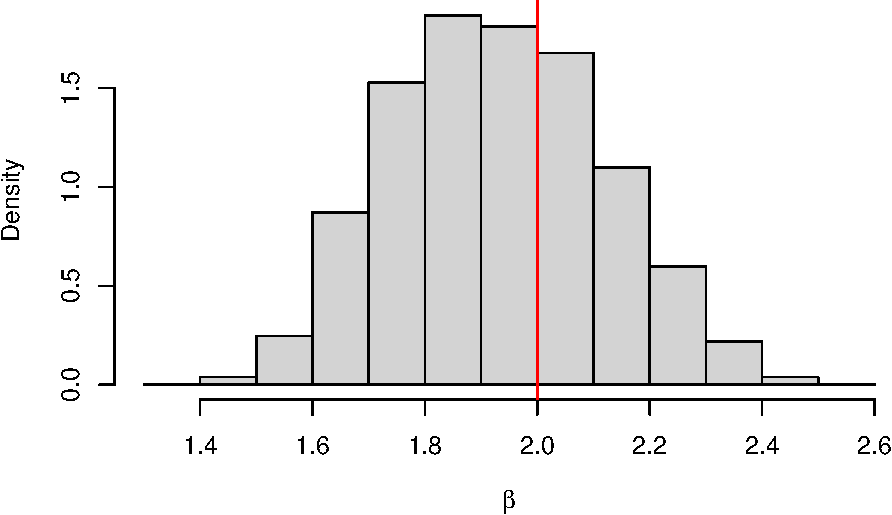
\includegraphics{_main_files/figure-latex/unnamed-chunk-54-1.pdf}

\begin{Shaded}
\begin{Highlighting}[]
\FunctionTok{mean}\NormalTok{(b.store, }\AttributeTok{na.rm =} \ConstantTok{TRUE}\NormalTok{)}
\end{Highlighting}
\end{Shaded}

\begin{verbatim}
## [1] 1.930908
\end{verbatim}

\begin{Shaded}
\begin{Highlighting}[]
\FunctionTok{quantile}\NormalTok{(b.store, }\FunctionTok{c}\NormalTok{(}\FloatTok{0.025}\NormalTok{, }\FloatTok{0.975}\NormalTok{), }\AttributeTok{na.rm =} \ConstantTok{TRUE}\NormalTok{)}
\end{Highlighting}
\end{Shaded}

\begin{verbatim}
##     2.5%    97.5% 
## 1.593348 2.302256
\end{verbatim}

\end{example}

\hypertarget{prior-ellicitation}{%
\section{Prior Ellicitation}\label{prior-ellicitation}}

Throughout this course, we have tried to be objective in our choice of prior distributions. We have discussed \textbf{uninformative} and \textbf{invariant} prior distributions. Sometimes we have used \textbf{vague} prior distributions, such as the Exp(0.01) distribution. And other times, we have left the parameters as generic values. This misses out on one real difference between Bayesian and frequentist inference. In Bayesian inference, we can include prior information about the model parameters. Determining the value of prior parameters is know as prior elicitation. This is more of an art than a science and still controversial in the Bayesian world. In this section, we are going to look at a few ways of how to elicit prior information from experts.

\begin{example}
This example to show how difficult it is to talk to experts in other areas about probabilities and risk. Suppose we are interested in estimating the number of crashes on a new motorway that is being designed. Denote the number of crashes per week by \(X\) and suppose \(X \sim \hbox{Po}(\lambda)\). We place a \(\lambda \sim \Gamma(\alpha, \beta)\) prior distribution on the rate parameter \(\lambda\). The density function of this prior distribution is
\[
\pi(\lambda) = \frac{\beta^\alpha}{\Gamma(\alpha)}\lambda^{\alpha-1}\exp(-\lambda\beta). 
\]
The parameter \(\alpha\) is know as the shape parameter and \(\beta\) the rate parameter.

We interview road traffic police, highway engineers and driving experts to estimate the values of \(\alpha\) and \(\beta\). The difficulty is that they do not know about the Gamma distribution or what shape and rate parameters are. Instead, we can ask them about summaries of the data. For the Gamma distribution, the mean is \(\alpha/\beta\), the mode is \((\alpha - 1)/\beta\) and the variance is \(\alpha/\beta^2\). If we can get information about two of these then we can solve for \(\alpha\) and \(\beta\). But needing two brings about another difficulty, non-mathematicians have limited understanding of statistics and probability. They can find it difficult to differentiate between the mean and the mode, and the concept of variance is very difficult to explain.
\end{example}

\hypertarget{prior-summaries}{%
\subsection{Prior Summaries}\label{prior-summaries}}

The first method we are going to look at is called summary matching. For this method, we ask experts to provide summaries of what they think the prior distribution is. We then choose a function form for the prior distribution and use these summaries to estimate the prior distribution. The choice of summaries depend on the application in hand as well as the choice of prior distribution. Common choices are: the mean, median, mode, variance, and cumulative probabilities (i.e.~\(\pi(\theta < 0.5)\)).

\begin{example}
Let's return to the motorway example from above. Suppose that a highway engineer tells us the expected number of crashes per week is 0.75 and the probability that \(\lambda < 0.9\) is 80\%. Matching summaries tells us
\[
\frac{\alpha}{\beta} = 0.75 \\
\int_0^{0.9}\pi(\lambda) d\lambda = 0.8
\]

From the expectation, we have \(\alpha = 0.7\beta\). To estimate the value of \(\beta\) from the cumulative probability, we need to find the root to the equation
\[
\int_0^{0.9} \frac{\beta^{0.75\beta}}{\Gamma(\beta)}\lambda^{0.75\beta-1}e^{-\lambda\beta}d\lambda - 0.8 = 0. 
\]

This looks horrible, but there are many optimisation ways to solve this problem.

\begin{Shaded}
\begin{Highlighting}[]
\NormalTok{cummulative.eqn }\OtherTok{\textless{}{-}} \ControlFlowTok{function}\NormalTok{(b)\{}
  \CommentTok{\#Compute equation with value beta = b}
\NormalTok{  value }\OtherTok{\textless{}{-}} \FunctionTok{pgamma}\NormalTok{(}\FloatTok{0.9}\NormalTok{, }\FloatTok{0.75}\SpecialCharTok{*}\NormalTok{b, b)}\SpecialCharTok{{-}}\FloatTok{0.8}
  \FunctionTok{return}\NormalTok{(value)}
  
\NormalTok{\}}

\FunctionTok{uniroot}\NormalTok{(cummulative.eqn, }\AttributeTok{lower =} \DecValTok{1}\NormalTok{, }\AttributeTok{upper =} \DecValTok{1000}\NormalTok{)}
\end{Highlighting}
\end{Shaded}

\begin{verbatim}
## $root
## [1] 21.80224
## 
## $f.root
## [1] -5.747051e-08
## 
## $iter
## [1] 8
## 
## $init.it
## [1] NA
## 
## $estim.prec
## [1] 6.103516e-05
\end{verbatim}

This gives us \(\beta = 21.8\) and \(\alpha = 13.65\).
\end{example}

\hypertarget{betting-with-histograms}{%
\subsection{Betting with Histograms}\label{betting-with-histograms}}

The difficulty with the summary matching method is that it requires experts to describe probabilities about the prior parameter, which is difficult to do and quite an abstract concept. Instead of asking them to describe summaries, we can ask them to draw the prior distribution completely, using a betting framework.

In the \textbf{prior weights} (sometimes called roulette) method, we give the the experts a set of intervals for the parameter of interest and fixed number of coins. We then ask the experts to place the coins in the intervals according to how likely they think the parameter will be in each interval, effectively betting on what value the parameter will take. For example, they might place \(n_1\) coins in the interval \(\theta \in [a, b)\), \(n_2\) in \(\theta \in [b, c)\) and \(n_3\) for \(\theta \in \[c, d]\). From this we can construct our prior density.

\begin{example}
Suppose we are interested in the probability a pharmaceutical drug has the desired clinical effect. The outcome of each patient's treatment can be modelled by \(X\sim\hbox{Bernoulli}(p)\). We ask a clinical about their experience with patients and similar treatments. We ask the expert to estimate the probability of successful treatment by betting on the value for \(p\) using the following table and 20 coins.

\begin{longtable}[]{@{}ll@{}}
\toprule\noalign{}
\(p\) & Coins \\
\midrule\noalign{}
\endhead
\bottomrule\noalign{}
\endlastfoot
{[}0, 0.2) & 3 \\
{[}0.2, 0.4) & 7 \\
{[}0.4, 0.6) & 5 \\
{[}0.6, 0.8) & 3 \\
{[}0.8, 1{]} & 2 \\
\end{longtable}

We can use the website \url{http://optics.eee.nottingham.ac.uk/match/uncertainty.php\#} to fit a distribution to this table. It proposes the best fit of a \(p \sim \Gamma(3.10, 6.89)\). We can use this distribution as the prior distribution, although it is not conjugate and places weight on \(p > 1\). Another option is a Beta\((1.64, 2.16)\) distribution,
\end{example}

\hypertarget{prior-intervals}{%
\subsection{Prior Intervals}\label{prior-intervals}}

The last method we will look at is the \textbf{bisection} method. In this method, we ask the experts to propose four intervals, each of which the parameter value is likely to fall into, i.e.~\(\pi(\theta \in [a, b)) = \pi(\theta \in [c, d)) = \pi(\theta \in [e, f))= \pi(\theta \in [g, h)) = 0.25\). From these intervals, we develop a prior distribution that fits these intervals.

\begin{example}
The police are interested in estimating the number of matching features between a fingerprint from a crime scene and a fingerprint from a suspect in the police station. The number of matching features is \(X \sim \hbox{Po}(\lambda)\). We speak to experienced fingerprint analysts. She advises us that about a quarter of the time, she would expect to see between 0 and 4 matches and this is when it is unlikely for the suspect to be the criminal. She says in some cases, it's very clear that the suspect is the criminal as she would expect to see 20 to 30 matches. The rest of the time, she sees some matches but the fingerprint collected at the crime scene is poor quality, so see may see 5 to 14 matches. She agrees that the matches are uniform across this range. So our four intervals are {[}0, 4{]}, {[}5, 12{]}, {[}13, 19{]}, {[}20, 30{]}. Using the Match software, we get a Uniform{[}0, 30{]} distribution.
\end{example}

\hypertarget{lab-3}{%
\section{Lab}\label{lab-3}}

\hypertarget{gaussian-processes-1}{%
\subsection{Gaussian Processes}\label{gaussian-processes-1}}

\begin{example}
The code below shows how to set up a Gaussian Process and draw samples from it in R.

\begin{Shaded}
\begin{Highlighting}[]
\FunctionTok{require}\NormalTok{(MASS)}
\end{Highlighting}
\end{Shaded}

\begin{verbatim}
## Loading required package: MASS
\end{verbatim}

\begin{Shaded}
\begin{Highlighting}[]
\NormalTok{squared.exponential.covariance }\OtherTok{\textless{}{-}} \ControlFlowTok{function}\NormalTok{(x1, x2, alpha, ell) \{}
  \CommentTok{\#Squared Exponential Covariance Function}
  \CommentTok{\#Inputs: x1, x2 {-}{-} vectors, alpha, ell {-}{-} variance and length scale parameter}
\NormalTok{  pairwise\_distances }\OtherTok{\textless{}{-}} \FunctionTok{outer}\NormalTok{(x1, x2, }\StringTok{"{-}"}\NormalTok{)}
\NormalTok{  covariance\_matrix }\OtherTok{\textless{}{-}}\NormalTok{ alpha }\SpecialCharTok{*} \FunctionTok{exp}\NormalTok{(}\SpecialCharTok{{-}}\FloatTok{0.5} \SpecialCharTok{*}\NormalTok{ (pairwise\_distances }\SpecialCharTok{/}\NormalTok{ ell)}\SpecialCharTok{\^{}}\DecValTok{2}\NormalTok{)}
  \FunctionTok{return}\NormalTok{(covariance\_matrix)}
\NormalTok{\}}

\CommentTok{\#Set up GP}
\NormalTok{x }\OtherTok{\textless{}{-}} \FunctionTok{seq}\NormalTok{(}\DecValTok{0}\NormalTok{, }\DecValTok{5}\NormalTok{, }\FloatTok{0.01}\NormalTok{)}
\NormalTok{mu }\OtherTok{\textless{}{-}} \FunctionTok{rep}\NormalTok{(}\DecValTok{0}\NormalTok{, }\FunctionTok{length}\NormalTok{(x))}
\NormalTok{Sigma }\OtherTok{\textless{}{-}} \FunctionTok{squared.exponential.covariance}\NormalTok{(x, x, }\DecValTok{1}\NormalTok{, }\DecValTok{1}\NormalTok{)}

\CommentTok{\#Generate Samples and Summaries}
\NormalTok{f }\OtherTok{\textless{}{-}}\NormalTok{ MASS}\SpecialCharTok{::}\FunctionTok{mvrnorm}\NormalTok{(}\DecValTok{1000}\NormalTok{, mu, Sigma)}
\NormalTok{f.mean }\OtherTok{\textless{}{-}} \FunctionTok{apply}\NormalTok{(f, }\DecValTok{2}\NormalTok{, mean) }\CommentTok{\#GP mean}
\NormalTok{f.}\FloatTok{95.}\NormalTok{upper }\OtherTok{\textless{}{-}} \FunctionTok{apply}\NormalTok{(f, }\DecValTok{2}\NormalTok{, quantile, }\FloatTok{0.975}\NormalTok{)}
\NormalTok{f.}\FloatTok{95.}\NormalTok{lower }\OtherTok{\textless{}{-}} \FunctionTok{apply}\NormalTok{(f, }\DecValTok{2}\NormalTok{, quantile, }\FloatTok{0.025}\NormalTok{)}

\CommentTok{\#Generate some plots}
\FunctionTok{plot}\NormalTok{(x, f[}\DecValTok{1}\NormalTok{, ], }\AttributeTok{type =} \StringTok{\textquotesingle{}l\textquotesingle{}}\NormalTok{, }\AttributeTok{ylim =} \FunctionTok{c}\NormalTok{(}\FunctionTok{min}\NormalTok{(f[}\DecValTok{1}\SpecialCharTok{:}\DecValTok{3}\NormalTok{, ]), }\FunctionTok{max}\NormalTok{(f[}\DecValTok{1}\SpecialCharTok{:}\DecValTok{3}\NormalTok{, ])))}
\FunctionTok{lines}\NormalTok{(x, f[}\DecValTok{2}\NormalTok{, ], }\AttributeTok{col =} \DecValTok{2}\NormalTok{)}
\FunctionTok{lines}\NormalTok{(x, f[}\DecValTok{3}\NormalTok{, ], }\AttributeTok{col =} \DecValTok{3}\NormalTok{)}
\end{Highlighting}
\end{Shaded}

\includegraphics{_main_files/figure-latex/unnamed-chunk-56-1.pdf}

\begin{Shaded}
\begin{Highlighting}[]
\FunctionTok{plot}\NormalTok{(x, f.mean, }\AttributeTok{type =} \StringTok{\textquotesingle{}l\textquotesingle{}}\NormalTok{, }\AttributeTok{ylim =} \FunctionTok{c}\NormalTok{(}\SpecialCharTok{{-}}\DecValTok{5}\NormalTok{, }\DecValTok{5}\NormalTok{)) }\CommentTok{\#0 {-}{-} no surprise there}
\FunctionTok{polygon}\NormalTok{(}\FunctionTok{c}\NormalTok{(x, }\FunctionTok{rev}\NormalTok{(x)), }\FunctionTok{c}\NormalTok{(f.}\FloatTok{95.}\NormalTok{lower, }\FunctionTok{rev}\NormalTok{(f.}\FloatTok{95.}\NormalTok{upper)), }\AttributeTok{col =} \FunctionTok{rgb}\NormalTok{(}\DecValTok{0}\NormalTok{, }\DecValTok{0}\NormalTok{, }\DecValTok{1}\NormalTok{, }\FloatTok{0.25}\NormalTok{))}
\end{Highlighting}
\end{Shaded}

\includegraphics{_main_files/figure-latex/unnamed-chunk-56-2.pdf}
\end{example}

\begin{exercise}

Code up example 6.1. How does your choice of length scale affect the posterior distribution. You can use

\begin{Shaded}
\begin{Highlighting}[]
\NormalTok{x }\OtherTok{\textless{}{-}} \SpecialCharTok{{-}}\DecValTok{5}\SpecialCharTok{:}\DecValTok{5}
\NormalTok{y }\OtherTok{\textless{}{-}}  \FunctionTok{c}\NormalTok{(}\FloatTok{3.0942822}\NormalTok{, }\FloatTok{3.0727920}\NormalTok{, }\FloatTok{2.6137341}\NormalTok{, }\FloatTok{1.8818820}\NormalTok{, }\FloatTok{1.2746738}\NormalTok{, }\FloatTok{1.2532116}\NormalTok{, }\FloatTok{1.4620830}\NormalTok{, }\FloatTok{1.4194647}\NormalTok{, }\FloatTok{1.6786969}\NormalTok{, }\FloatTok{1.1057042}\NormalTok{, }\FloatTok{0.4118125}\NormalTok{)}
\end{Highlighting}
\end{Shaded}

with \(\sigma^2 = 0.2\).To draw samples from the multivariate normal distribution with mean vector \(\boldsymbol{\mu}\) and covariance matrix \(\Sigma\) use

\begin{Shaded}
\begin{Highlighting}[]
\NormalTok{mvnorm.chol }\OtherTok{\textless{}{-}} \ControlFlowTok{function}\NormalTok{(mu, Sigma)\{}
  \CommentTok{\#Multivariate Normal Sampler with Cholesky Input}
  \CommentTok{\#Inputs: mu {-}{-} mean, chol {-}{-} covariance matrix}
\NormalTok{  Sigma.chol }\OtherTok{\textless{}{-}} \FunctionTok{chol}\NormalTok{(Sigma }\SpecialCharTok{+} \FloatTok{0.0001}\SpecialCharTok{*}\FunctionTok{dim}\NormalTok{(Sigma)[}\DecValTok{1}\NormalTok{])}
  \FunctionTok{return}\NormalTok{(mu }\SpecialCharTok{+} \FunctionTok{t}\NormalTok{(Sigma.chol)}\SpecialCharTok{\%*\%}\FunctionTok{rnorm}\NormalTok{(}\FunctionTok{length}\NormalTok{(mu)))  }
\NormalTok{\}}
\end{Highlighting}
\end{Shaded}

\end{exercise}

\begin{exercise}
Repeat Exercise 6.1, but this time set the fine grid to be \(\boldsymbol{x}^* = \{-5, -4.9, -4.8, \ldots, 9.8, 9.9, 10\}\). What happens to the posterior distribution after \(x^* = 5\)?
\end{exercise}

\begin{exercise}
You observe the following data

\begin{Shaded}
\begin{Highlighting}[]
\NormalTok{x }\OtherTok{\textless{}{-}} \SpecialCharTok{{-}}\DecValTok{5}\SpecialCharTok{:}\DecValTok{5}
\NormalTok{y }\OtherTok{\textless{}{-}} \FunctionTok{cos}\NormalTok{(}\FloatTok{0.5}\SpecialCharTok{*}\NormalTok{x) }\SpecialCharTok{+} \FunctionTok{log}\NormalTok{(x }\SpecialCharTok{+} \DecValTok{6}\NormalTok{)}
\NormalTok{y}
\end{Highlighting}
\end{Shaded}

\begin{verbatim}
##  [1] -0.8011436  0.2770003  1.1693495  1.9265967  2.4870205  2.7917595
##  [7]  2.8234927  2.6197438  2.2679618  1.8864383  1.5967517
\end{verbatim}

\begin{Shaded}
\begin{Highlighting}[]
\FunctionTok{plot}\NormalTok{(x, y, }\AttributeTok{xlab =} \StringTok{"x"}\NormalTok{, }\AttributeTok{ylab =} \StringTok{"f(x)"}\NormalTok{, }\AttributeTok{ylim =} \FunctionTok{c}\NormalTok{(}\DecValTok{0}\NormalTok{, }\DecValTok{4}\NormalTok{))}
\end{Highlighting}
\end{Shaded}

\includegraphics{_main_files/figure-latex/unnamed-chunk-59-1.pdf}

Fit a function to the data using a GP prior distribution. Note that this time there is no noise.
\end{exercise}

\hypertarget{missing-data}{%
\subsection{Missing Data}\label{missing-data}}

\begin{exercise}
In Example 6.2, suppose the observed data is \(\{y_1, y_2, y_3, y_4\} = \{4, 4, 5 ,2\}\). Design and code an MCMC algorithm to generate samples from the posterior distribution for \(p\) and \(y_5\).
\end{exercise}

\begin{exercise}
Suppose you manage a clinical trial. You administer a new drug to patients and record how many days until their symptoms are alleviated. You observe the times for the first 9 patients

\begin{Shaded}
\begin{Highlighting}[]
\NormalTok{x }\OtherTok{\textless{}{-}} \FunctionTok{c}\NormalTok{(}\DecValTok{33}\NormalTok{,  }\DecValTok{17}\NormalTok{, }\DecValTok{218}\NormalTok{,   }\DecValTok{3}\NormalTok{,  }\DecValTok{39}\NormalTok{,   }\DecValTok{3}\NormalTok{,  }\DecValTok{43}\NormalTok{,  }\DecValTok{14}\NormalTok{,  }\DecValTok{20}\NormalTok{)}
\end{Highlighting}
\end{Shaded}

Patient 10 drops out of the trial on day 50 and at this point, their symptoms have not changed. They send an email on day 200 to say they no longer have any symptoms (i.e.~\(x_i \in [50, \ldots, 200]\). Write down a model for this problem and derive the posterior distribution. Design and code an MCMC algorithm to generate samples from the posterior distribution for any model parameters and \(x_{10}\).
\end{exercise}

\hypertarget{approximate-bayesian-computation-1}{%
\subsection{Approximate Bayesian Computation}\label{approximate-bayesian-computation-1}}

\begin{exercise}
You observe the following data from an \(N(5, \sigma^2)\) distribution.

\begin{verbatim}
-5.93,  33.12, -21.41, -12.42, -17.64,  -5.47, -27.95, -22.25, -20.40, -26.28, -24.57,  
3.06,  44.28, 6.02, -21.14,  14.79, -15.10, 53.18,  38.61,   5.71
\end{verbatim}

Use an Exp(0.1) prior distribution on \(\sigma^2\) and develop a summary statistic ABC algorithm to draw samples from the approximate posterior distribution.
\end{exercise}

\begin{exercise}
You observe the following data from an \(Exp(\lambda)\) distribution.

\begin{verbatim}
2.6863422, 8.8468112, 8.8781831, 0.2712696, 1.8902442
\end{verbatim}

Use an \(Beta(1, 3)\) prior distribution on \(\lambda\) and develop an ABC algorithm to draw samples from the approximate posterior distribution. Write the ABC algorithm as a function so you can run it for different values of \(\varepsilon\). Run your algorithm for \(\varepsilon = \{20, \ldots, 100\}\) and record the approximate posterior median. Plot the relative error in your estimate against the true value of lambda, which is 0.2.
\end{exercise}

  \bibliography{book.bib,packages.bib}

\end{document}
